\documentclass[12pt]{report}			% Začátek dokumentu
\usepackage{MP}	
\usepackage{czech}
% Import stylu
\author{Amálie Jirotková}
\title{Diverzita dívek na~technických }
%\title2{vysokých školách a~žen v~IT}
\date{14. února 2023}
\vedouci{Dr.rer.nat. Michal Kočer}
\place{V Českých Budějovicích}
\skolnirok{2022/2023}
\logo{\includegraphics[width=16cm][scale=1.25]{GJ8_logotyp}}

\begin{document}
\pagenumbering{roman}                  % číslování stránek římskými číslicemi
	    \mytitlepage   % Vygenerování titulní strany
    	
    	\prohlaseni{
    		Prohlašuji, že jsem tuto práci vypracoval samostatně s vyznačením všech použitých pramenů.
    	}	
    	
    	\abstrakt{
    	
    	Z důvodu automatizace se bude měnit náplň práce zaměstnanců, proto je potřeba o tomto tématu začít mluvit. Dále je nezbytné zjistit stav diverzity a nezaostávat, tedy motivovat mladé a rekvalifikovat starší ženy a dívky pro ICT směr. Přesvědčení o dopadu na následné studium středoškoláků je vizualizována v praktické části. Šteření bylo provedeno formou dotazníku.
    		% Abstrakt
    	}{
    	
    	diverzita, dívky, ženy, vysoká škola, zaměstnání, Czechitas
    					% Klíčová slova
    	}
    	
    	\podekovani{
    	Chtěla bych poděkovat vedoucímu své práce za užitečné rady. Dále pak děkuji i neziskové organizaci Czechitas za možnost účasti na projektu a jejímu přizpůsobení ku prospěchu mé práce.
    					% Poděkování
    	}
	
   \tableofcontents\newpage			% Obsah
	
\addtocounter{page}{1}		% Posunutí counteru stránek
\pagenumbering{arabic}		% Číslování stránek arabskými číslicemi
	\chapter*{Úvod}
	
    	Maturitní práce se zaobírá diverzitou dívek na~informatických (ICT) vysokých školách~a~žen v~IT a~o~jejich obecném zájmu o~tyto technologie. Část zaměřená na~dívky se zaobírá volbou vysoké školy a~následného výběru zaměstnání. U~žen jsou středem zájmu obecná data o~zastoupení na~technických pozicích. 
    
        Maturitní práci jsem si vybrala, jelikož je mi toto téma velmi blízké. Chtěla bych nejen tímto způsobem motivovat zmíněnou cílovou skupinu k zájmu o~technologie a~o vzdělávání v~tomto směru, z toho důvodu jsem se rozhodla pod záštitou neziskové organizace Czechitas věnovat přednáškám pro středoškoláky na~toto téma.
        

      %\section*{Hypotézy}
      %\begin{itemize}
       %   \item Pandemie měla vliv na~studenty a~studentky ve výběru vysoké školy. O~proti minulým letům se navýšil nejen počet studentů, kteří podali přihlášku na~informatickou vysokou školu, ale i~procento dívek, a~to jak v~počtu poslaných přihlášek, tak v~počtu přijatých studentek
        %  \item Na~získání práce v~IT má větší vliv úroveň dosaženého vzdělání a~pohlaví, než věk.
         % \item Přednášky ovlivní alespoň jednu dívku, která před přednáškou neuvažovala o~studiu informatiky.
      %\end{itemize}

    %\chapter*{Cíle maturitní práce}	
        %Cíle maturitní práce - upozornění na~problematiku (zhodnocení momentální situace), informovat o~organizacích zabývající se touto problematikou, snaha  o~přiblížení dívkám na~středních školách studium informatické VŠ (ověřit dotazníkem).
	
\part{Diverzita trhu}
	
	\chapter{Uvedení do problematiky}
		  % Uvedení, proč je vůbec potřeba na~tento problém řeší, co ženy do IT přináší apod.
		  V České republice je pro 76\% podniků problém obsadit ICT odborníky. Tato situace není jen u nás, ale z dat, která máme k dispozici, můžeme říct, že je skoro ve všech státech Evropské Unie. Ze celé EU jsme na tom ale nejhůře. Pro porovnání např.: na Slovensku má obdobný problém pouze 59\% firem. Což je od výrazně blíže evropskému průměru 55\% podniků. Nejlépe jsou na tom v tomto směru zaměstnavatelé ve Španělsku, kde se s problémem nedostatku zaměstnanců tomto oboru potýká pouze 25\%, což je prakticky 3x méně než u nás.\cite{EmploymentOfICTSpecialists}
		  
		\section{Automatizace budoucích pracovních pozic a~nedostatek ICT odborníků}
            O budoucnost v tomto oboru se zajímalo například Světové ekonomické fórum, nezisková organizace, která byla založena pro spolupráci veřejného a soukromého sektoru. Jedná se o organizaci, založenou v roce 1971 v Ženevě. Je považována za nezávislou a není vázána na žádné zvláštní zájmy. Pod hlavičkou této skupiny, která se spojila i jinými firmami, vznikl dokument s názvem Future of jobs\footnote{Budoucnost zaměstnání} pojednávající o tématu budoucnosti v zaměstnání do 5 let od vydání, tedy do roku 2025. Na celém projektu se podílely organizace jako LinkedIn, Coursera, FutureFit AI aj.\cite{WorldEconomicForumInfo}
            
            Podle výsledků dotazníků z výše zmíněného dokumentu v závislosti na popularizaci automatizace a pandemii Covid-19 43\% dotazovaných podniků uvádí snížení počtu zaměstnanců v důsledku integrace technologií. Zároveň je zde 34\% podniků, které plánují rozšíření počtu zaměstnanců v důsledku integrace technologií. Do roku 2025 tedy bude čas strávený na běžných pracovních úkolech lidmi a stroji stejný. Změní se ale náplň zaměstnanců. Jako nejjednodušší a také nejlevnější řešení je podle odborníků rekvalifikace nastávajících zaměstnanců. Tímto způsobem je snaha přesunout téměř 50\% pracovníků vytlačených technologickou automatizací. Na tento postup v současné době pouze 21\% podniků uvádí, že jsou schopny využít veřejné prostředky k podpoře jejich zaměstnanců prostřednictvím rekvalifikace a zvyšování kvalifikace. Bude tedy potřeba, aby veřejný sektor vytvořil pobídky pro investice do trhů a také poskytnout záchranné sítě pro přesunuté pracovníky při změně zaměstnání. Je také potřeba zaměřit se na dlouhodobý problém vzdělávání a odborné přípravy. Stále tu v budoucnu nastává problém s klesáním počtu pracovních míst. Přestože počet zrušených pracovních míst bude překonán počtem vytvořených tzv.\uv{pracovních míst zítřka}, na rozdíl od předchozích let se tvorba nových pracovních míst zpomaluje, zatímco jejich rušení zrychluje. Očekává se tedy, že pracovních pozic bude ubývat z původních 15.,4\% na 9\% (pokles o 6,4\%), ale zároveň nově vznikající profese budou z původních 7,8\% tvořit až 13,5\% (nárůst 5,7\%) z celkového počtu zaměstnanců respondentů z řad firem. Pokud odhady převedeme do čísel, může nastat situace, kdy bude do roku 2025 v důsledku změny dělby práce mezi lidmi a stroj vytlačeno 85 miliónů pracovních míst, na druhou stranu ale vznikne 97 miliónů prcovních míst, které ale budou přizpůsobeny práci se stroji a algoritmy. I přes to, že ve výsledku bude počet pracovních míst více, bude problém některé pozice naplnit.\cite{WorldEconomicForum}
            
        \section{Situace na~VŠ}
            % Problematika diverzity dívek na~informatických vysokých školách a na IT pozicích
            
            Vysoké školy a data z nich jsou dobrým nástrojem pro alespoň částečnou předpověď trhu následujících let. I přesto, že se nedá určit, zda si studenti daného oboru najdou v této oblasti i uplatněné, jsou tato data zajímavá pro porovnání s EU. Například podle dat z let 2013 až 2020 (obr.: \ref{fig:vs_EU}) víme, že zájemců o studium na vysokých školách všeho druhu roste a trh se tomu může začít přizpůsobovat. A to se týká i diverzity dívek. \cite{StudentsTeritaryEducation}
            \begin{figure}[h]
                \centering 
                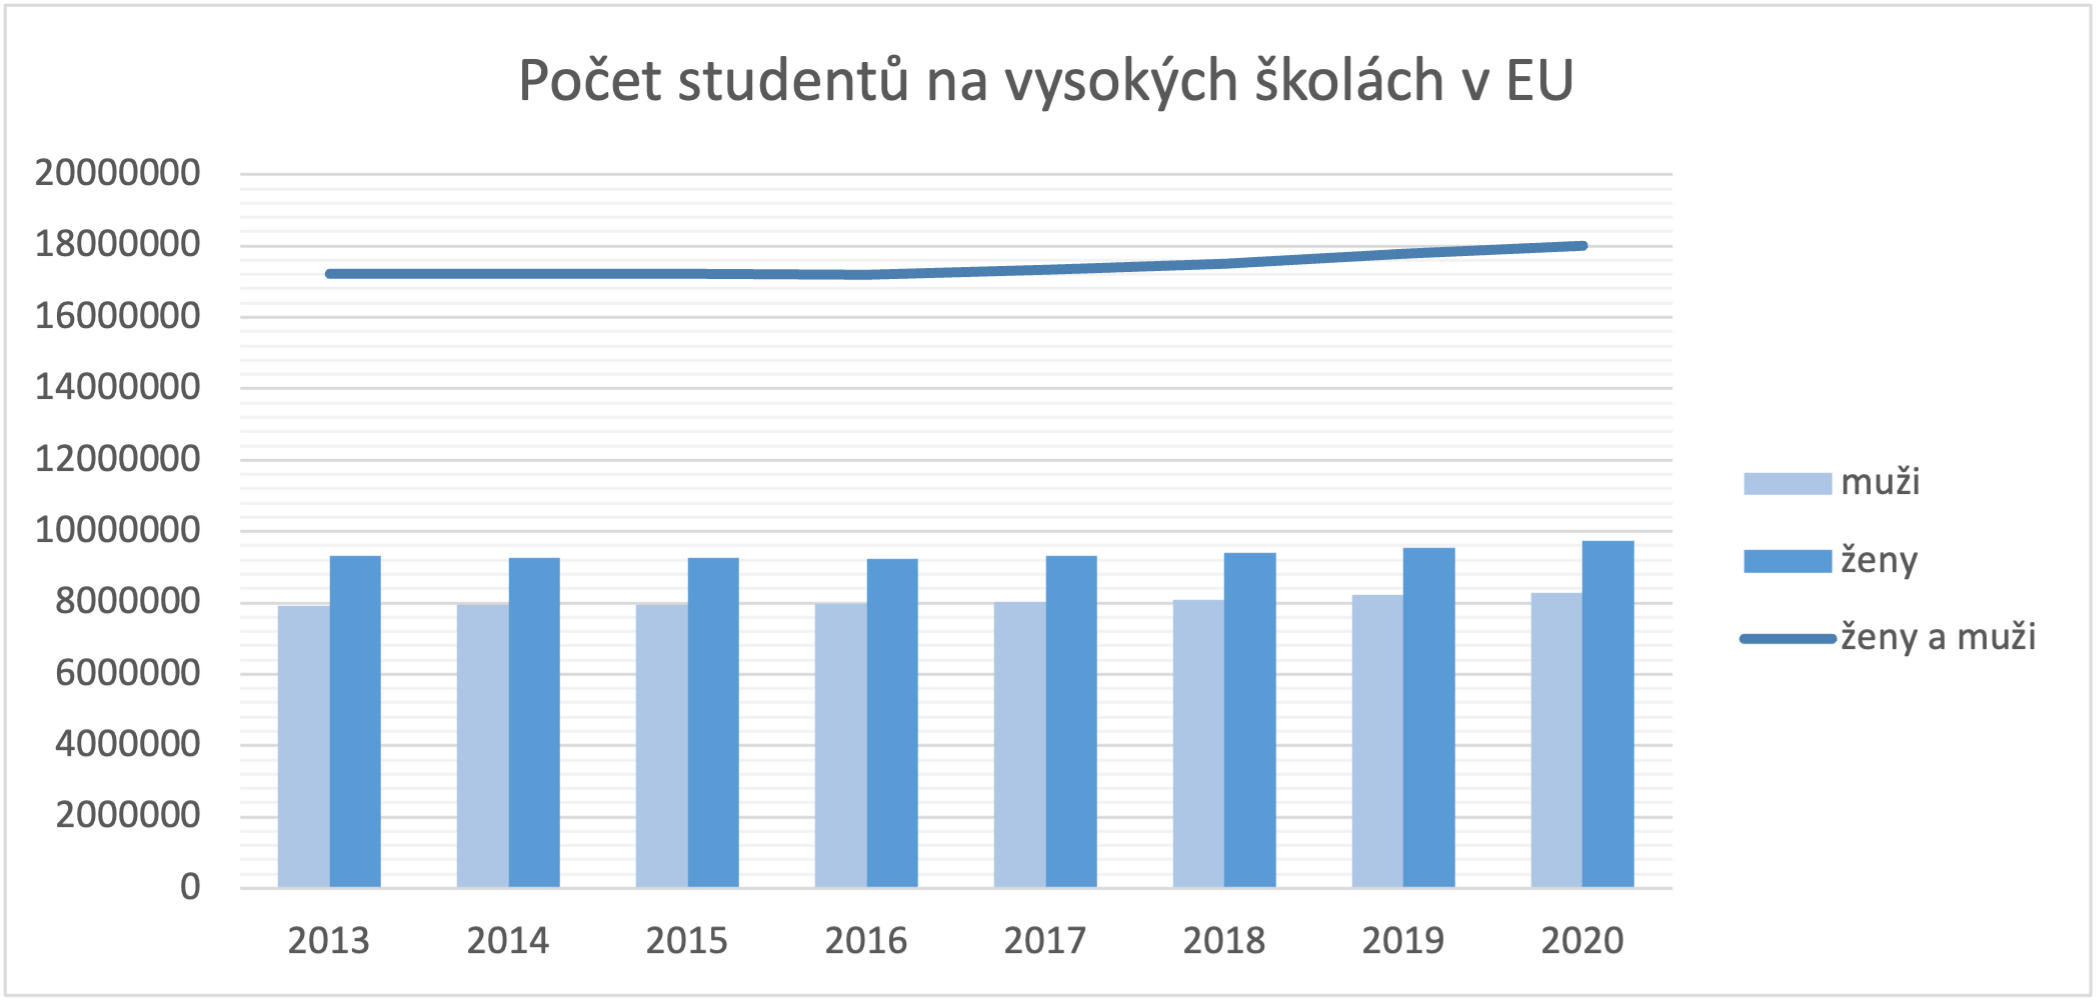
\includegraphics[width=16cm]{Maturitni Prace/images/vs_EU.png}
                \caption[Vizualizace diverzity na VŠ v EU 2013/20]{Vizualizace počtu studentů a jejich diverzita na VŠ v EU mezi lety 2013 a 2020; Zdroj:~Eurostat}
                \label{fig:vs_EU}
            \end{figure}

            Oproti tomu na vizualizovaných datech situace v ČR ze stejného časového období (obr.: \ref{fig:vs_CZ}) můžeme vidět relativně markantní pokles zájmu o studium všech vysokých škol. Je těžké určit příčinu poklesu, podle mého názoru je zde varianta, že se mladým lidem více vyplatí nastoupit do zaměstnání ihned po střední škole, kde získají potřebnou praxi a případně se budou učit potřebné specifické znalosti pro konkrétní pracovní pozici. Za to také může velmi rychlá doba, kdy ne všechny školy stíhají měnit kurikula jednotlivých oborů, tudíž po dostudování stejně může následovat období praxe, jelikož naučená látka už není aktuální. Toto nastává u rychle měnících se oborů jako je právě informatika. Pokles by se také dal propojit s pandemií Covid-19, toto období ale nekoreluje s daty, jelikož v EU pokles započal už v roce 2014, naopak by se dalo říct, že v období pandemie zájem o studium stagnoval. U studentek zájem o studium také klesá, procentuální rozdíl u naměřených hodnot za 7 let není moc patrný, ale trend je klesající.\cite{StudentsTeritaryEducation}
            
            \begin{figure}[h]
                \centering
                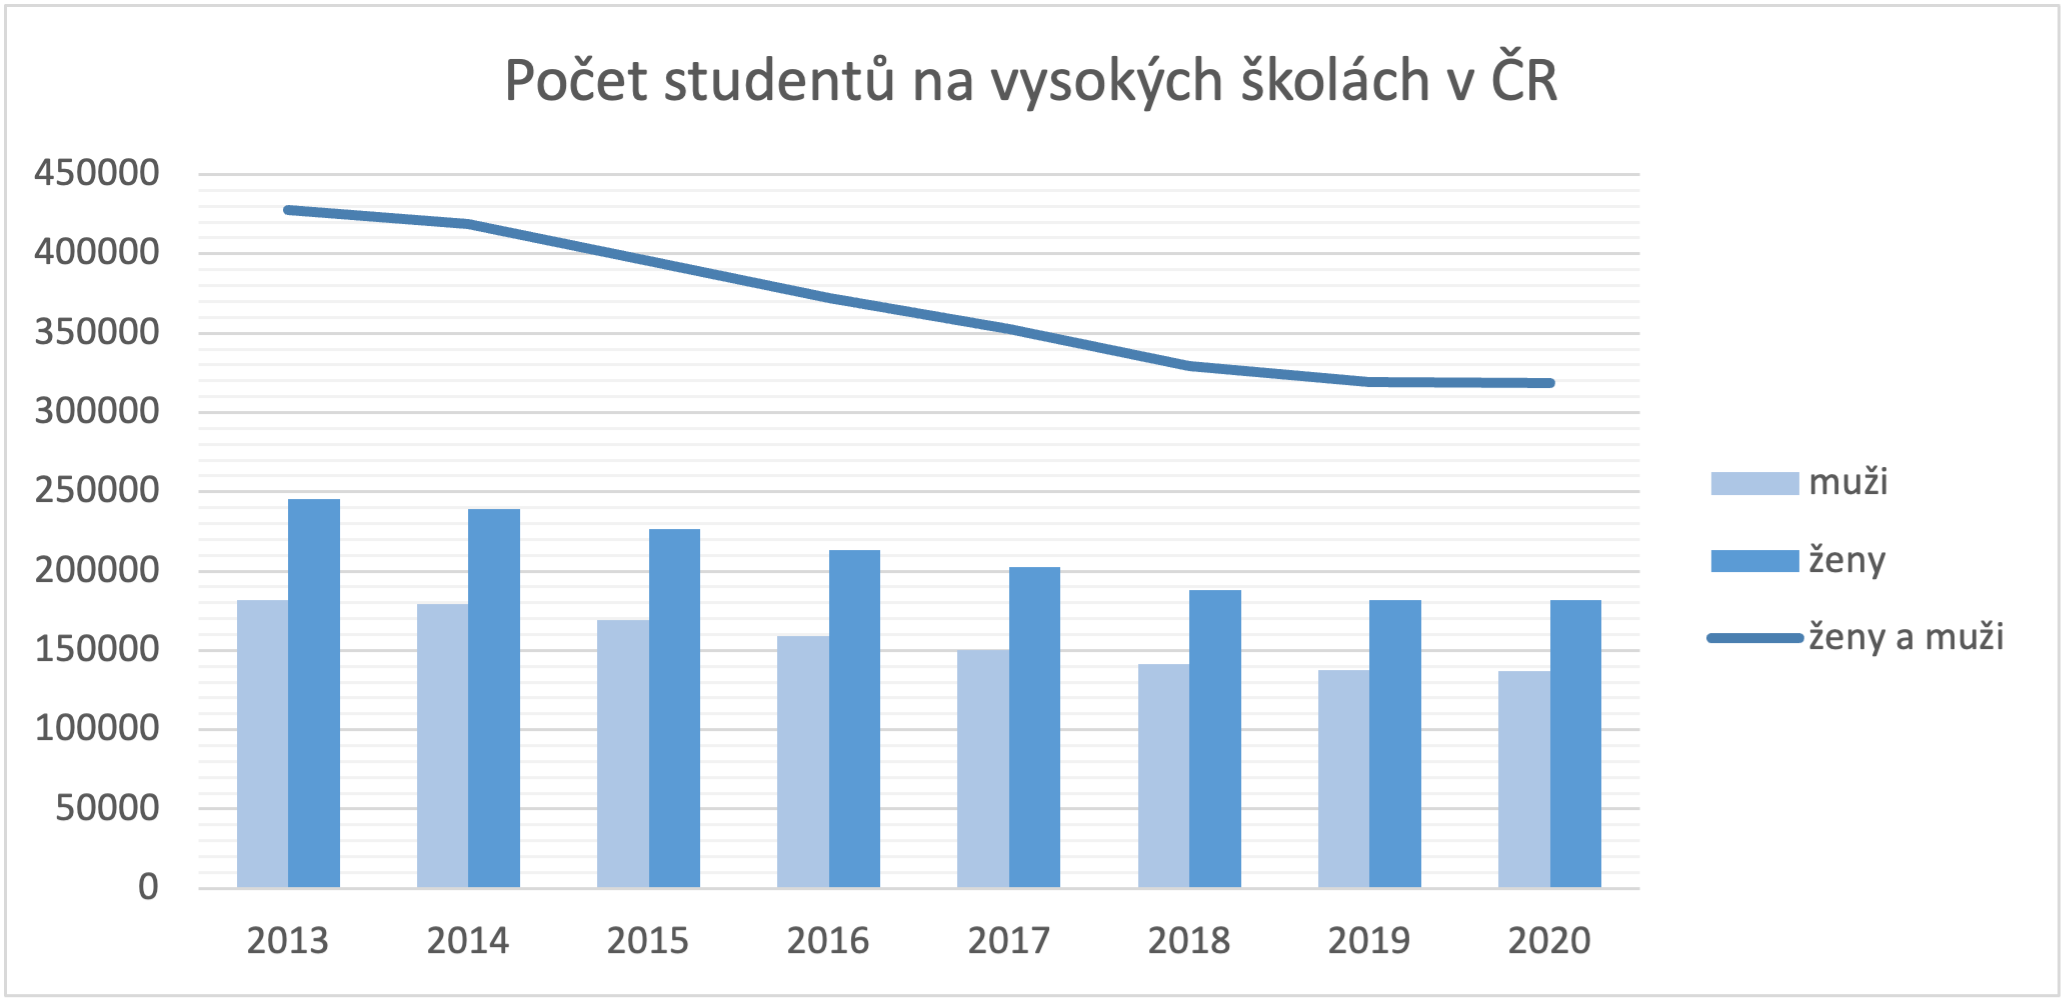
\includegraphics[width=16cm]{Maturitni Prace/images/vs_CZ.png}
                \caption[Vizualizace diverzity na VŠ v ČR 2013/20]{Vizualizace počtu studentů a jejich diverzita na VŠ v ČR mezi lety 2013 a 2020; Zdroj:~Eurostat}
                \label{fig:vs_CZ}
            \end{figure}
            
            Pokud se zaměříme jen na vysoké školy orientované na informační a komunikační technologie, je zde naopak možné vidět dlouhodobý nárůst zájmu a to od počátku měření. Mezi lety 2013 a 2020 se zájem o studium zvýšil o více než 30\% (obr.: \ref{fig:ICT_EU}). Největší zájem projevili studenti mezi lety 2016 a 2018, kde byl každoroční nárůst přibližně o 75 tisíc studentů v celé EU. Pokud se podíváme na diverzitu, je vidět, že u dívek je o tento směr stále menší zájem než u chlapců i přesto je zde nárůst mezi vykreslenými lety skoro 2\%. \cite{StudentsTeritaryEducation}
            
            \begin{figure}[h]
                \centering
                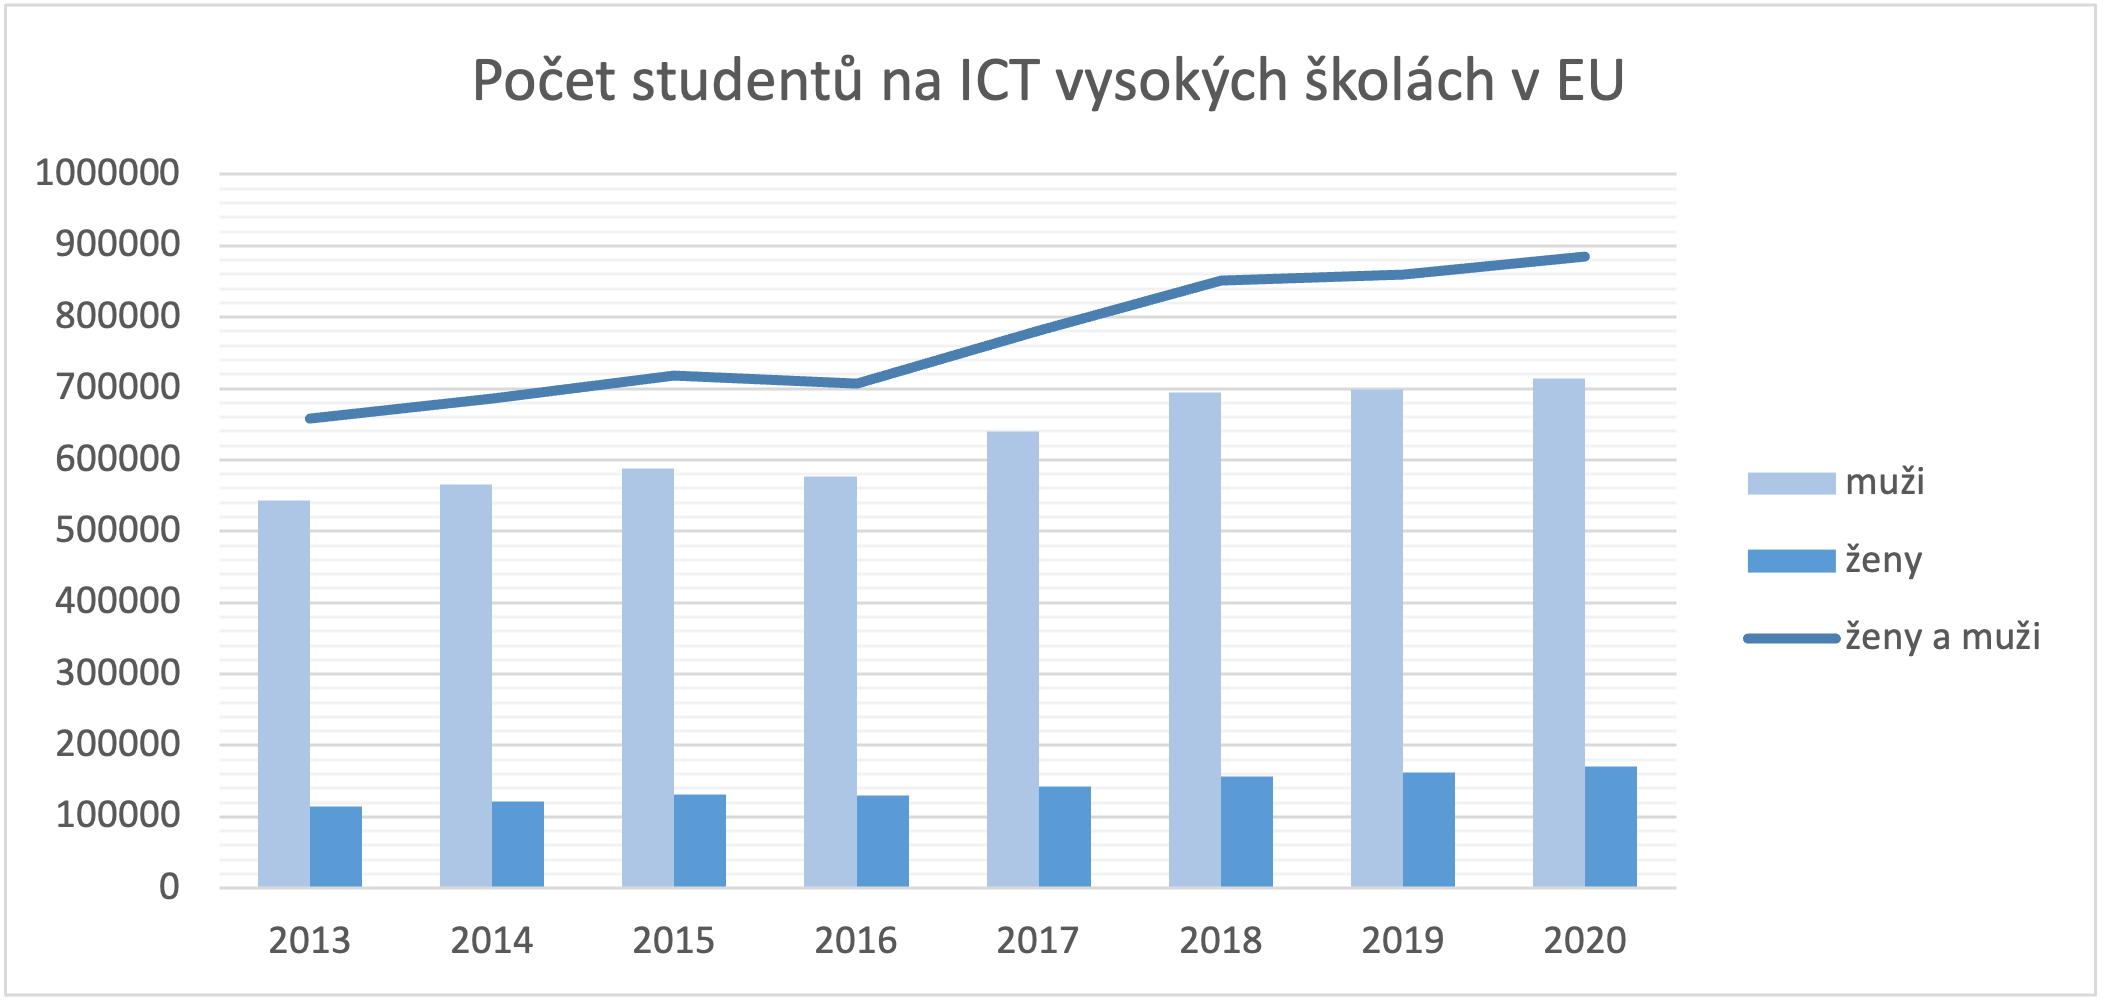
\includegraphics[width=16cm]{Maturitni Prace/images/ICT_EU.png}
                \caption[Vizualizace diverzity na ICT VŠ v EU 2013/20]{Vizualizace počtu studentů a jejich diverzita na ICT VŠ v EU mezi lety 2013 a 2020; Zdroj:~Eurostat}
                \label{fig:ICT_EU}
            \end{figure} 

            Když se opět zaměříme na situaci v České republice je statistika spíše opačná (obr.: \ref{fig:ICT_CZ}). Obecný zájem o studium informatických oborů na vysoké škole spíše stagnuje, mezi lety 2013 a 2016 byl trend klesající. Z grafu ale můžeme vyčíst, že v roce 2020 je vidět opět nárůst zájmu o tento obor. Stejně tomu je i u dívek, kde za vyobrazených 7 let vzrostl zájem z 15,1\% na 16,4\%, jde sice pouze o 1,3\%, což v porovnání s Evropským průměrem nezní nejlépe, na druhou stranu by situace mohla být výrazně horší. \cite{StudentsTeritaryEducation}
            \begin{figure}[h]
                \centering
                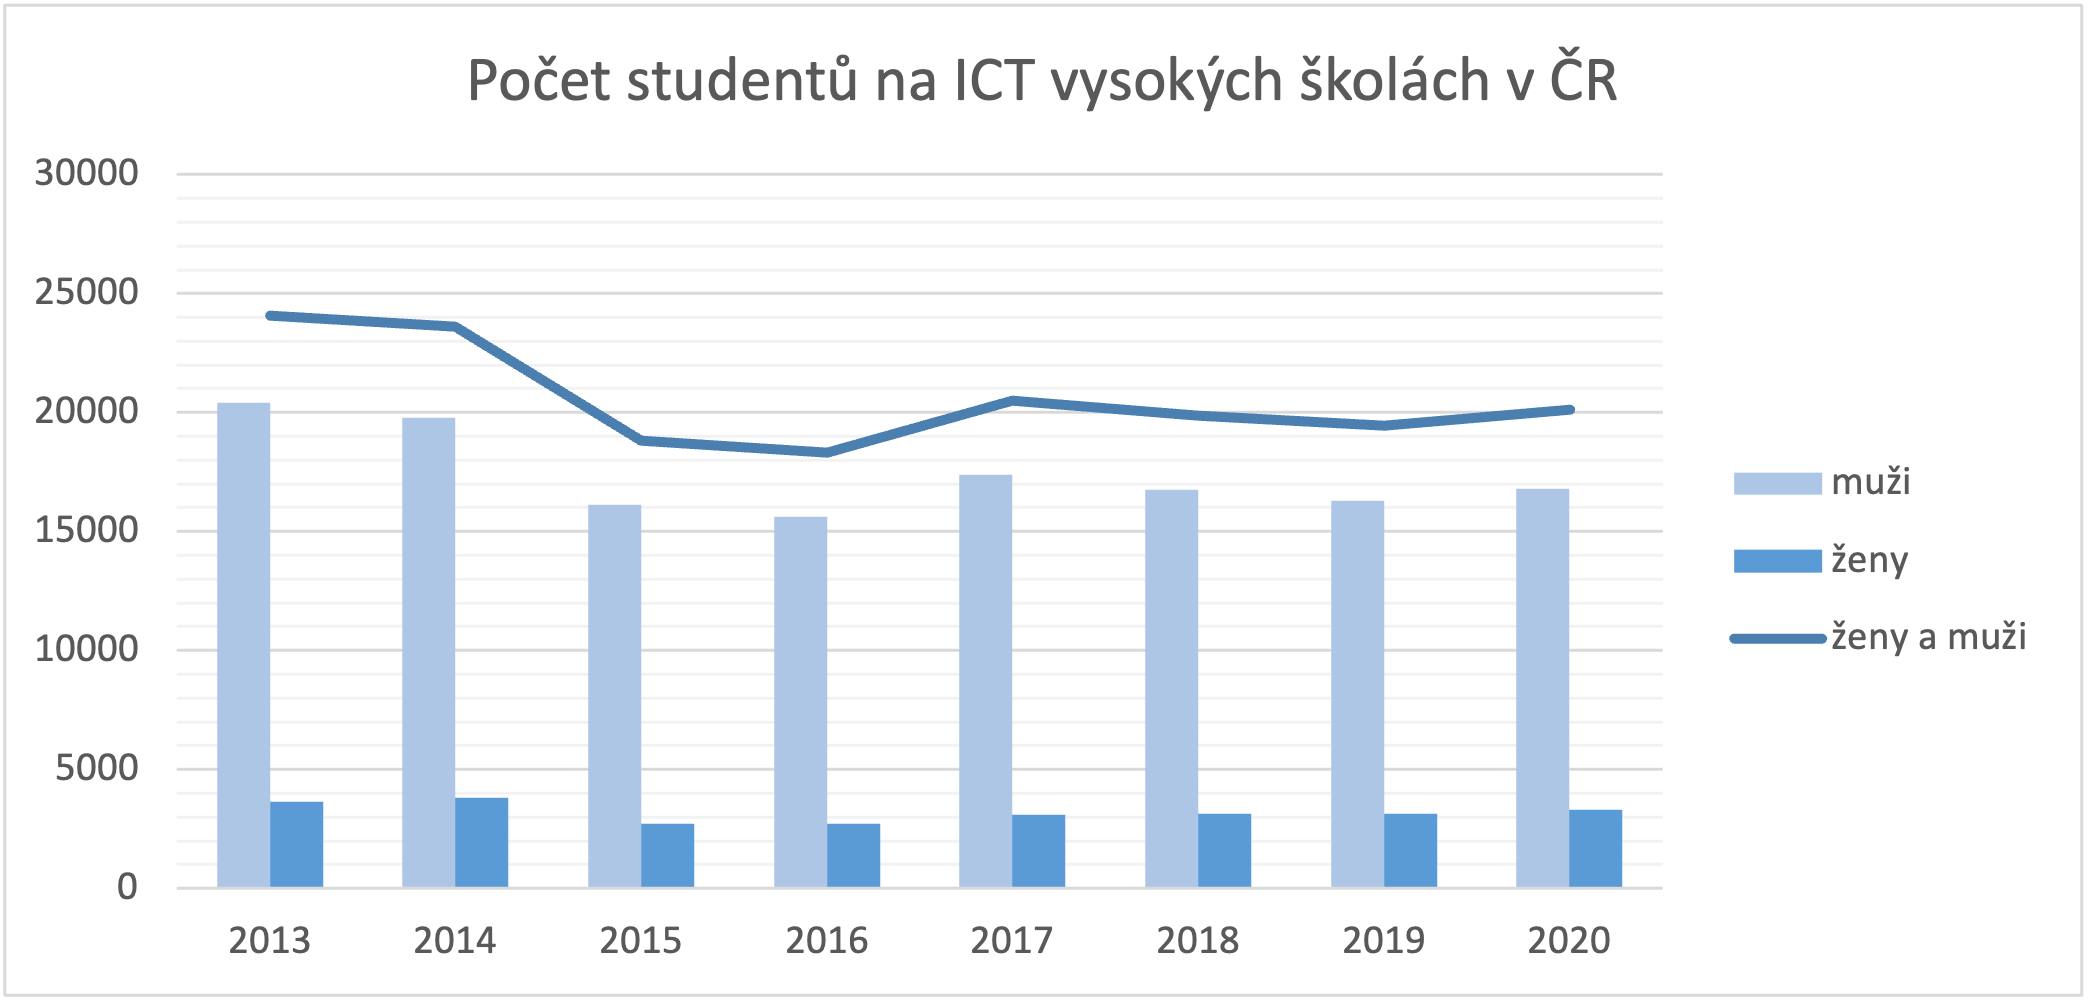
\includegraphics[width=16cm, height=8cm]{Maturitni Prace/images/ICT_CZ.png}
                \caption[Vizualizace diverzity na ICT VŠ v ČR 2013/20]{Vizualizace počtu a diverzity studentů na ICT VŠ v ČR mezi lety 2013 a 2020; Zdroj: Eurostat}
                \label{fig:ICT_CZ}
            \end{figure}
            
            \newpage
        \subsection {Vliv pandemie na~tuto problematiku}
            %jaký vliv na~přihlášky měla pandemie Covid 19 - hypotéza 
            
            Ve své práci jsem chtěla zahrnout také vliv pandemie Covid-19, jelikož během pár let změnil celý trh. V době pandemie se celý svět přesunul do online světa. Jelikož i studium přešlo do virtuálního světa, při psaní mé práce mě napadlo, že by bylo zajímavé zhodnotit, jestli mělo toto období i dopad na výběr vysoké školy a to převážně na dívky ve volbě informatických vysokých škol. Jelikož práce v ICT může být stabilnější. Pro porovnání jsem zvolila ČVUT, kde jsem vybrala Fakultu informačních technologií (FIT) a Fakultu elektrotechnickou (FEL), které mají právě informatické zaměření. 
            \begin{figure}[h]
                \centering
                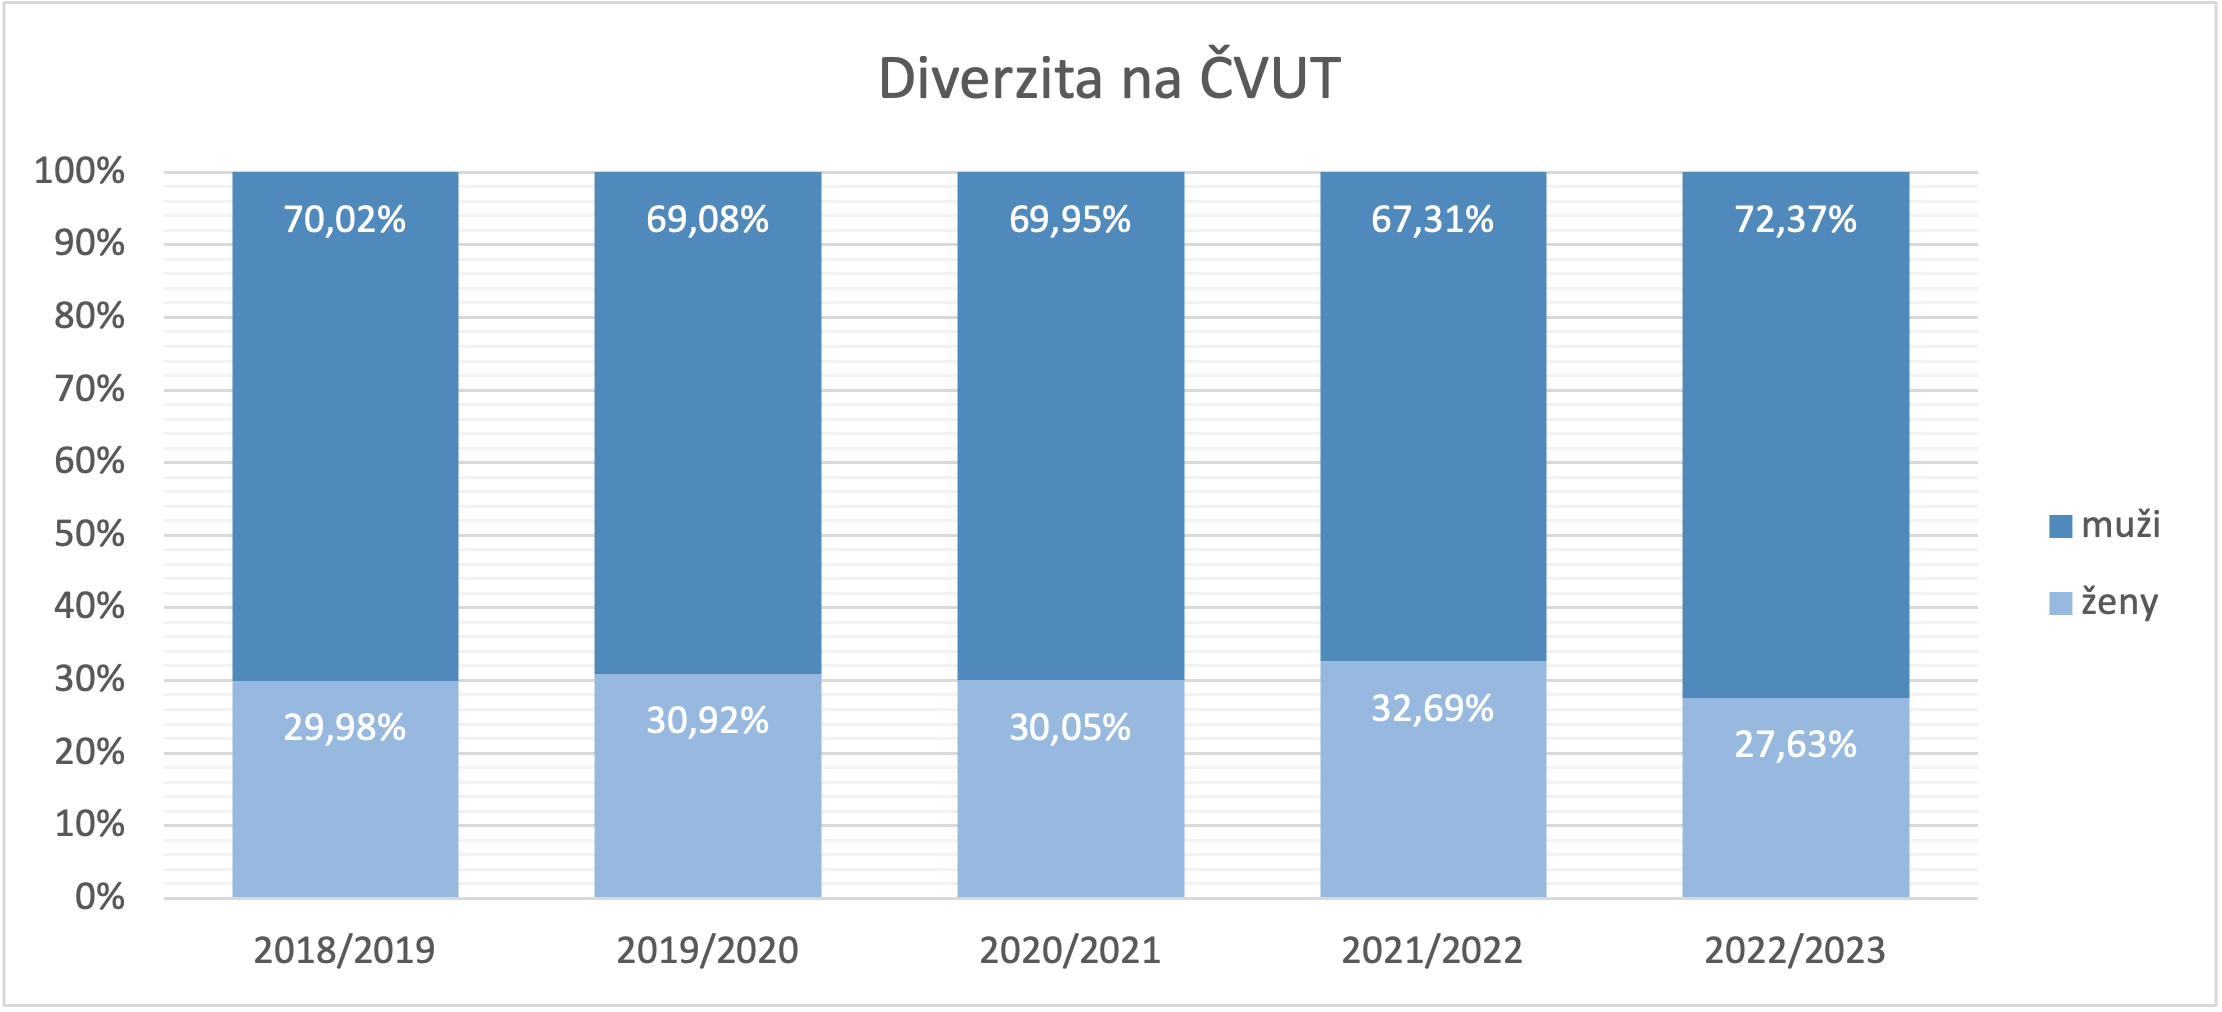
\includegraphics[width=16cm]{Maturitni Prace/images/proc_divek_CVUT_2018-22.png}
                \caption[Vizualizace diverzity na VŠ ČVUT 2018/20]{Rozdíl poslaných přihlášek dívkami na VŠ ČVUT mezi lety 2018 a 2022; Zdroj: ČVUT}
                \label{fig:proc_divek_CVUT_2018-22}
            \end{figure}
            
            Na začátek je důležité zmínit, že na grafu jsou vyobrazeny akademické roky, tedy přihlášky se posílají vždy na začátku uvedeného roku. Pro porovnání bych chtěla přiložit graf všechny dívkami odeslané přihlášky na všechny fakulty Českého vysokého učení technického v Praze (obr.: \ref{fig:proc_divek_CVUT_2018-22}). Jelikož pandemie Covid-19 vypukla v březnu roku 2020(\cite{Covid}). Předpokládala jsem, že největší vliv může mít na maturitní ročníky 2020/2021. Na rok předchozí v tomto směru pandemie ani nemohla mít velký vliv, jelikož v době vypuknutí probíhal uzávěr odesílání přihlášek na VŠ, tudíž většina o své vysoké škole měla rozhodnuto. Zajímavý je zároveň i celkový pokles v podaných přihláškách na rok 2022. \cite{CVUT} 
            \begin{figure}[h]
                \centering
                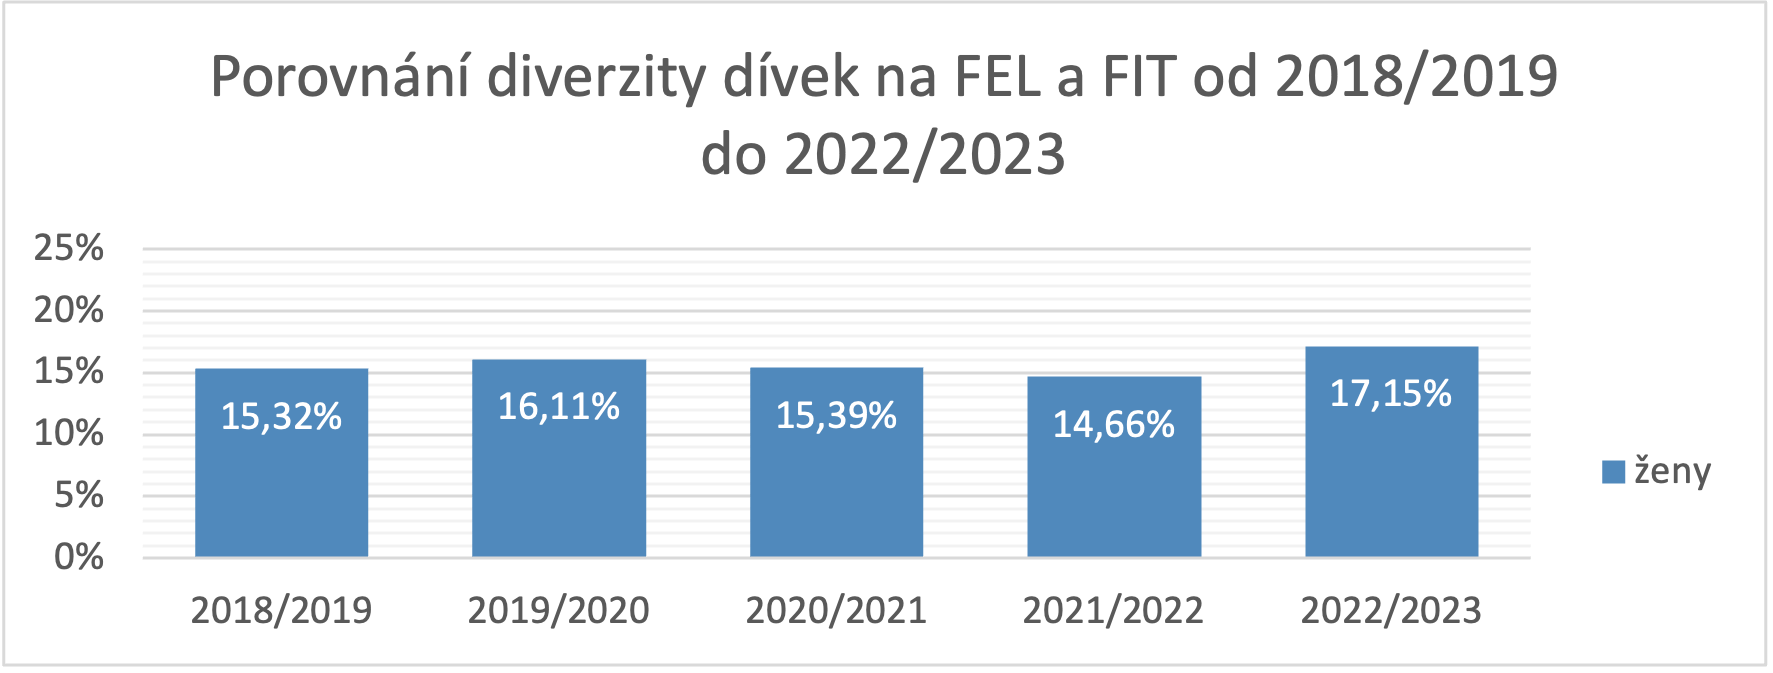
\includegraphics[width=16cm]{Maturitni Prace/images/proc_divek_FIT_FEL_2018-22.png}
                \caption[Vizualizace diverzity na FIT a FEL 2018/20]{Procentuální rozložení dívek na fakultách FIT a FEL mezi lety 2018 a 2022; Zdroj: ČVUT}
                \label{fig:proc_divek_FIT_FEL_2018-22}
            \end{figure}
            
            Když porovnáme počet odeslaných přihlášek dívkami na obě zmiňované fakulty - FIT a FEL (obr.: \ref{fig:proc_divek_FIT_FEL_2018-22}). Nárůst je zde patrný, ale až v akademickém roce 2022/23. Je tedy pravděpodobnější, že pandemie měla obecně větší vliv na přihlášení na vysoké školy, ale tento nárůst se neprojevil do tohoto odvětví. O rok později, kdy bylo možné více vidět následky pandemie a její vliv na trh práce se rozhodli studenti tomuto oboru věnovat. 
            
            \begin{figure}[h]
                \centering
                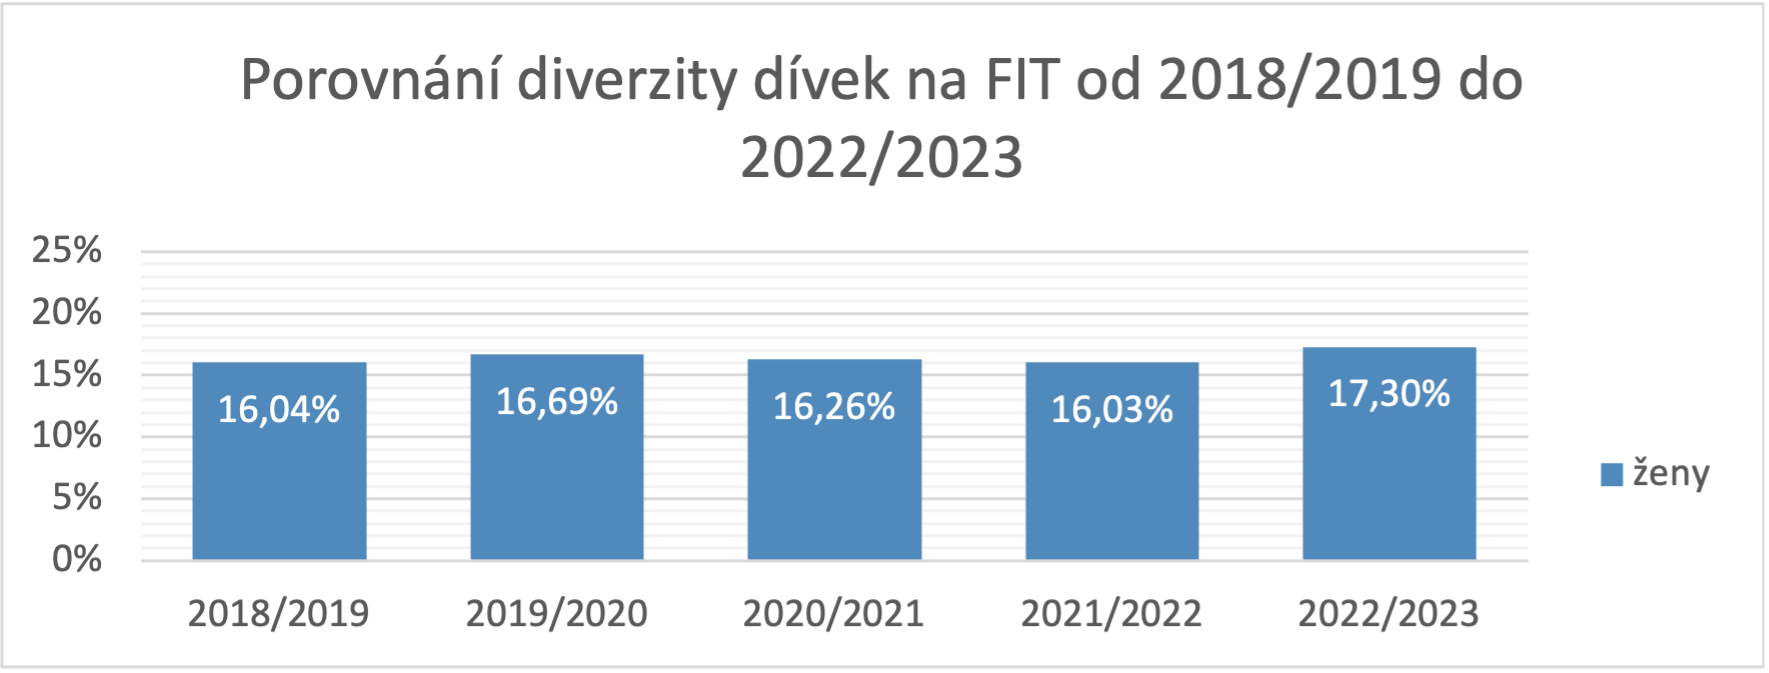
\includegraphics[width=16cm]{Maturitni Prace/images/proc_divek_FIT_2018-22.png}
                \caption[Vizualizace diverzity na FIT 2018/20]{Diverzita dívek na fakultě FIT mezi lety 2018 a 2022; Zdroj: ČVUT}
                \label{fig:proc_divek_FIT_2018-22}
            \end{figure}
            
            Po zjištění, jak hodnoty rostou, porovnáme situaci na jednotlivých fakultách (obr.: \ref{fig:proc_divek_FIT_2018-22}, \ref{fig:proc_divek_FEL_2018-22}), zde se ukázalo, že v akademickém roce 2021/22 na FIT bylo více dívek než na FEL, ale o rok později se tato data vyrovnala a situace je na obou fakultách podobná.
            
            To jestli za těmito výkyvy stojí právě pandemie Covid-19 se nedá úplně potvrdit, ale zároveň ani vyvrátit, jelikož je zde výrazně více faktorů, která rozhodování studentů mohlo ovlivnit. Jedním z nich může být také věk přihlášených studentů, mohlo se tedy přihlásit více bývalých studentů a rozhodnout se jít tímto směrem, anebo také \uv{síla ročníku}. Z dostupných dat je ale zřejmé, že zde v následujících letech po tomto období nárůst je, a to nejen na informatických vysokých školách, zda je ale pandemie přímou příčinou dokázat nemůžeme.
            
            Zároveň je také potřeba uvažovat i do budoucna, jelikož v grafech (obr.: \ref{fig:proc_divek_CVUT_2018-22}, \ref{fig:proc_divek_FIT_FEL_2018-22}, \ref{fig:proc_divek_FIT_2018-22}, \ref{fig:proc_divek_FEL_2018-22}) jsou vyobrazena pouze data počtu podaných přihlášek. Nepotvrzuje to reálný počet studentů v tomto oboru. Na tuto statistiku bohužel nemám dostatek dat.
            
            \begin{figure}
                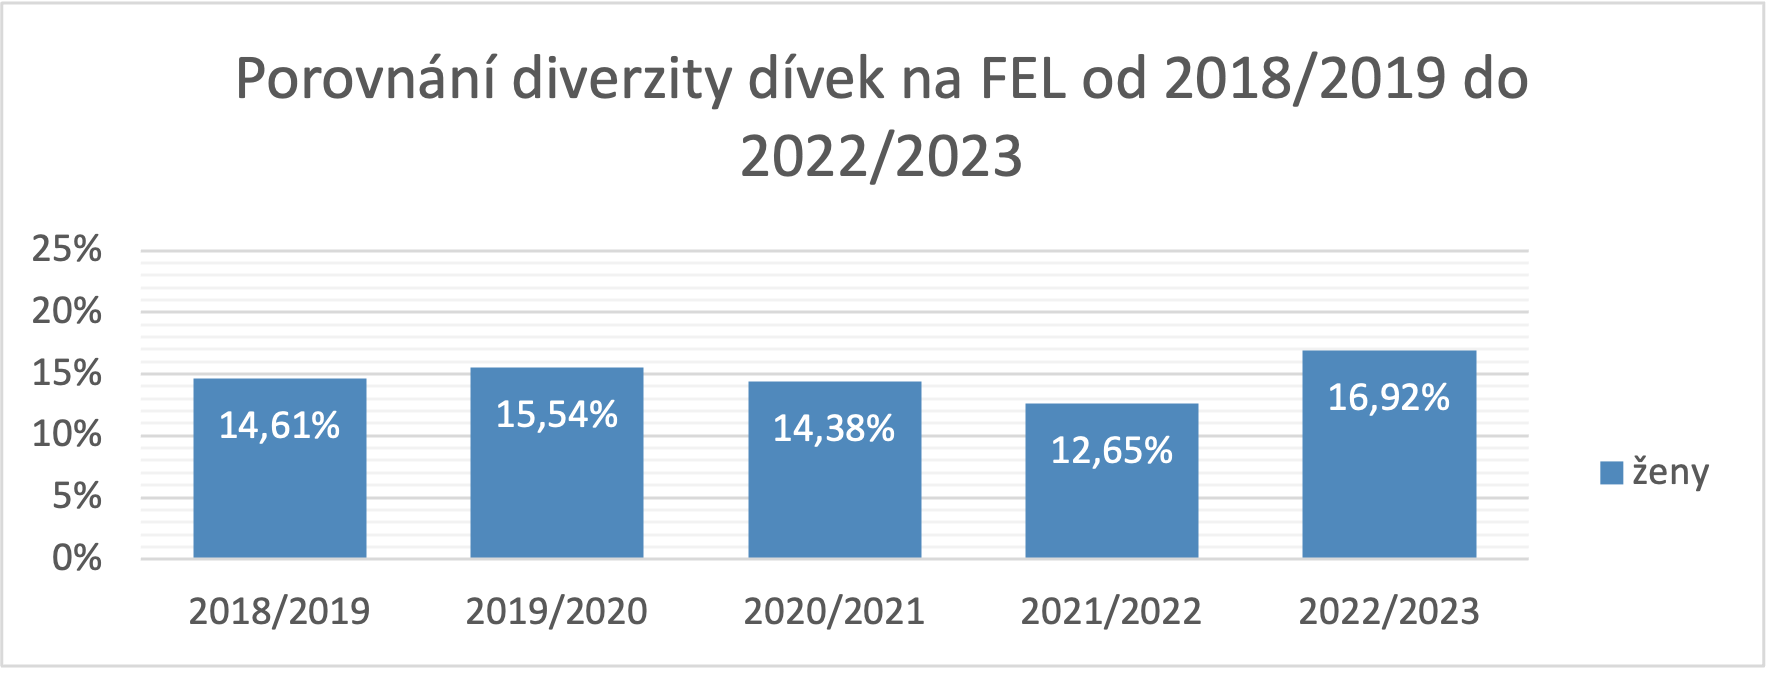
\includegraphics[width=16cm]{Maturitni Prace/images/proc_divek_FEL_2018-22.png}
                \caption[Vizualizace diverzity na FEL 2018/20]{Diverzita dívek na fakultě FEL mezi lety 2018 a 2022; Zdroj: ČVUT}
                \label{fig:proc_divek_FEL_2018-22}
            \end{figure}
            
            
    
    \chapter{Analýza diverzity}
    	
        \section{Studenti ICT na~vysokých školách v České republice}
            V~roce 2020 studovalo vysokou školu přibližně 300 tisíc osob, nejvíce to pak bylo v roce 2010, kdy se~počet studentů dostal až na~hodnotu 396 tisíc (obr.: \ref{fig:studenti_VS}). Od~roku 2010 pak počet neustále klesal, mezi lety 2019 až 2020 však zájem o~vysoké školy narostl o~11 tisíc studentů. Co se týká studentů ICT oborů, ty také dosáhly největšího maxima okolo roku 2010, což bylo cirka 26 tisíc studentů. Naopak nejméně bylo studentů těchto oborech v~roce 2017, od té doby ale toto číslo neustále roste, v roce 2020 se jeho hodnota dostala skoro k 22 tisícům osob. V porovnání se~všemi studenty vysokých škol se jedná o~7,2\%, toto číslo bylo před 19 lety poloviční. Během tohoto období toto číslo nikdy neklesalo, jen rostlo či mírně stagnovalo.~\cite{LidskeZdrojeVIT}
           
            \begin{figure}[h]
                \centering
                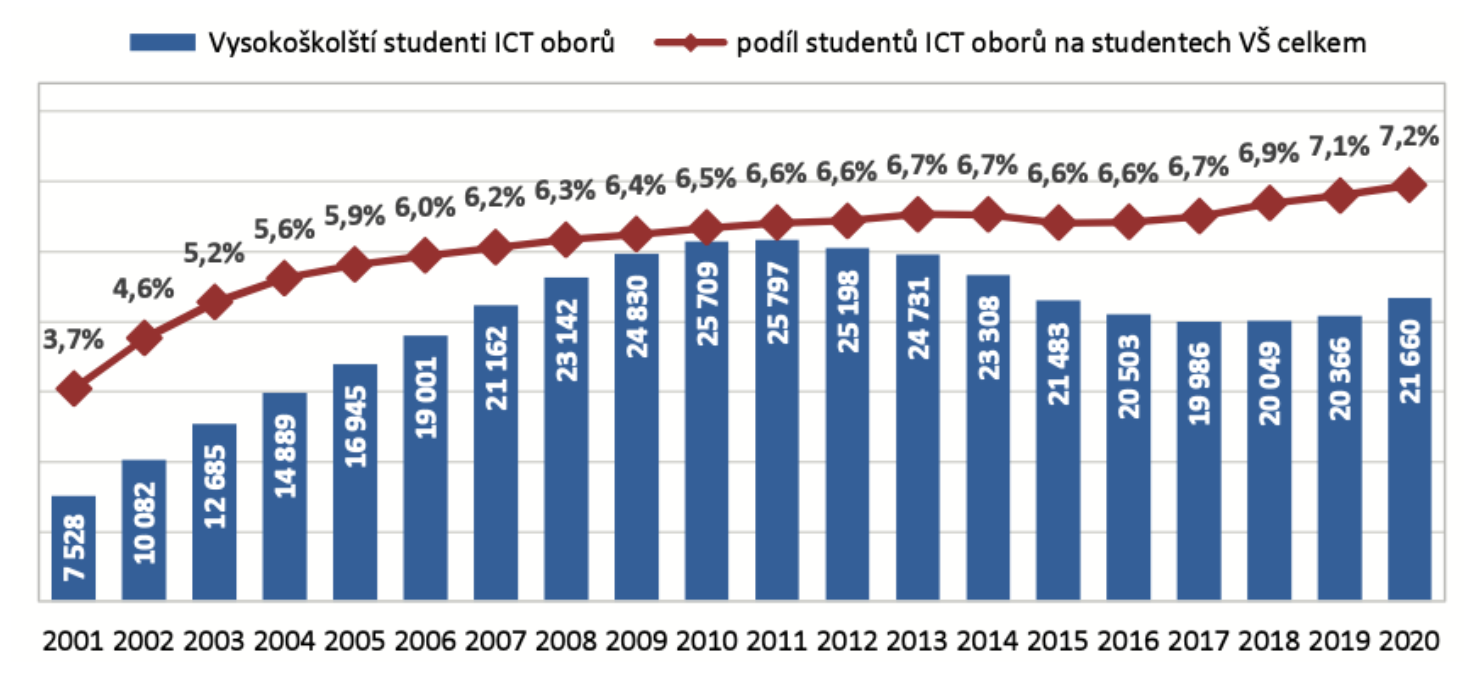
\includegraphics[width=16cm]{Maturitni Prace/images/studenti_VS.png}
                \caption[Rozložení studentů na ICT VŠ v 2020]{Procento studentů na ICT školách a jejich počet v ČR v roce 2020; Zdroj: ČSÚ/MŠMT}
                \label{fig:studenti_VS}
            \end{figure}
            
            Co se pak týká absolventů z~těchto vysokých škol, situace je procentuálně podobná jen se zpožděním pár let (obr.: \ref{fig:absolventi_VS}). Z posledních dat z~roku 2020 v tomto oboru absolvovalo skoro 3700 studentů, což je 5,8\% z~celkových absolventů na~VŠ.\cite{LidskeZdrojeVIT}
            
            \begin{figure}[h]
                \centering
                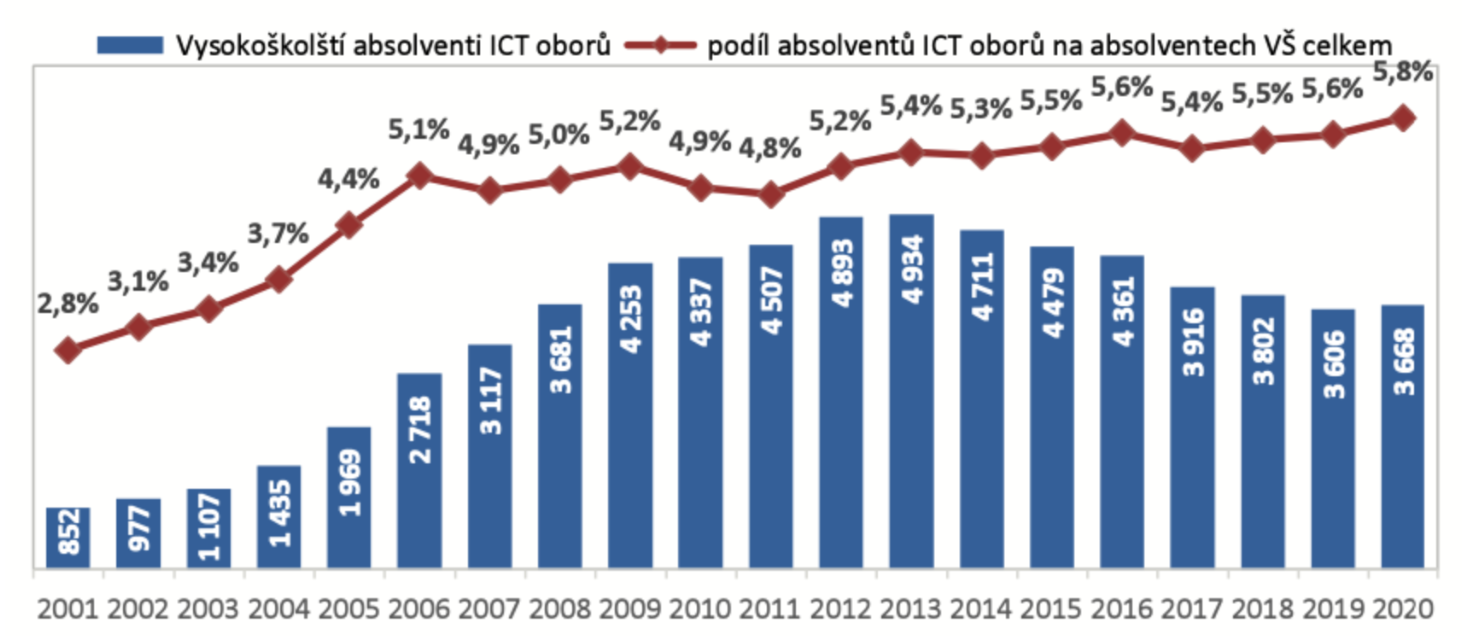
\includegraphics[width=16cm]{Maturitni Prace/images/absolventi_VS.png}
                \caption[Rozložení studentů na ICT VŠ podle oborů a stupňů studia 2013/20]{Rozložení studentů na ICT VŠ podle oborů a stupňů studia v roce 2020; Zdroj: ČSÚ/MŠMT} 
                \label{fig:absolventi_VS}
            \end{figure}
            
            \subsection{Rozložení studentů na ICT oborech na vysokých školách v České republice}
                    
                Studenty ICT od sebe dělí dva hlavní obory, nejvíce zastoupený mezi nimi je Vývoj a analýza softwaru a aplikací. Tento obor je oblíbený ve všech stupních studia a to více než u poloviny studentů (obr.: \ref{fig:studijni_obor_VS}). Dalším velmi zastoupenými obory studijního programu v celkovém součtu studentů jsou Interdisciplinární programy a kvalifikace (24\%), Návrhy a správa databází a sítí (7\%) zbylá 3\% pak zbyla na studenty studující ICT obory jinde nezařazené. \cite{LidskeZdrojeVIT}
                
                \begin{figure}[h]
                    \centering
                    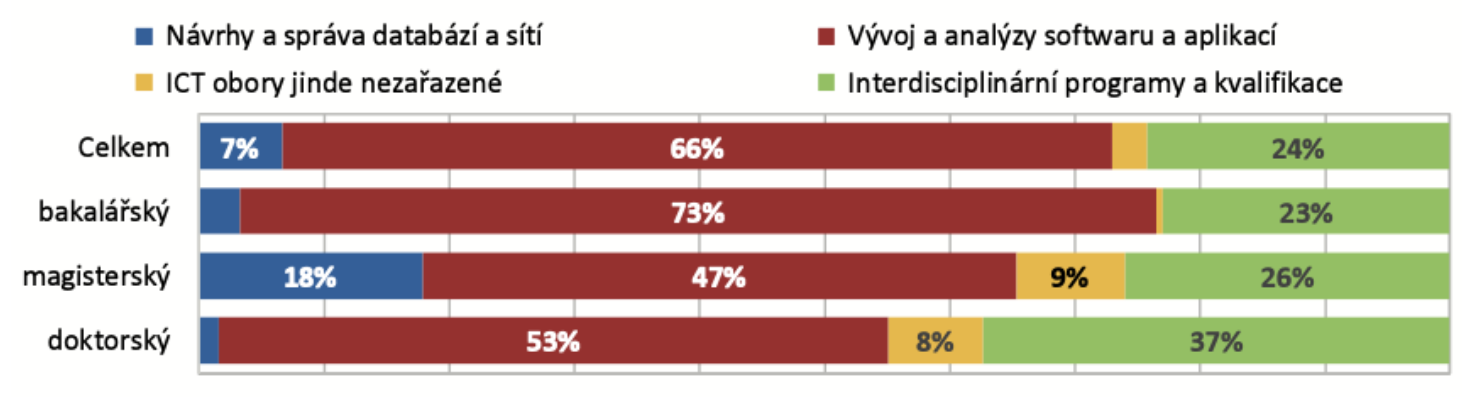
\includegraphics[width=16cm]{Maturitni Prace/images/studijni_obor_VS.png}
                    \caption[Rozložení studentů VŠ podle oborů v roce 2020]{Rozložení studentů VŠ podle oborů v roce 2020; Zdroj: ČSÚ/MŠMT}
                    \label{fig:studijni_obor_VS}
                \end{figure}
                
                Co se týká diverzity dívek na všech vysokých školách v tomto oboru je trend na dobré cestě (obr.: \ref{fig:pohlavi_VS}). V roce 2020 bylo na ICT obory přihlášeno 17\% dívek. Není to mnoho, ale při porovnání se situací v roce 2010 je zde zlepšení o 5\%. Při srovnání se všemi studijními programy na vysokých školách je převaha žen nad muži 56:44, v takovém případě je ale 17\% výrazně málo.\cite{LidskeZdrojeVIT}
                
                \begin{figure}[h]
                    \centering
                     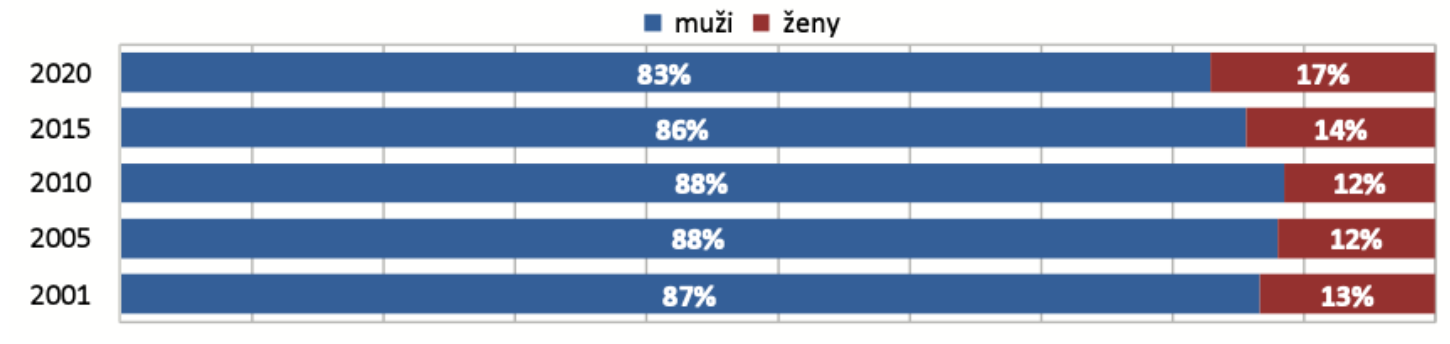
\includegraphics[width=16cm]{Maturitni Prace/images/pohlavi_VS.png}
                    \caption[Diverzita studentů ICT vysokých škol v roce 2020 v ČR]{Diverzita studentů ICT vysokých škol v roce 2020 v ČR; Zdroj: ČSÚ/MŠMT}
                    \label{fig:pohlavi_VS}
                \end{figure}
  
            \subsection{Zahraniční studenti ICT oborů na vysokých školách v České republice}
            
                V České republice také studují zahraniční studenti, jejich počet každoročně roste o několik procent (obr.: \ref{fig:obcanstvi_VS}). V letech 2010 tvořilo procento zahraničních studentů na ICT oborech na našich vysokých školách pouze 13\%, zatímco v roce 2020 se toto číslo více než zdvojnásobilo, tou dobou zde studovalo 29\% zahraničních studentů. 
                \begin{figure}[h]
                    \centering
                     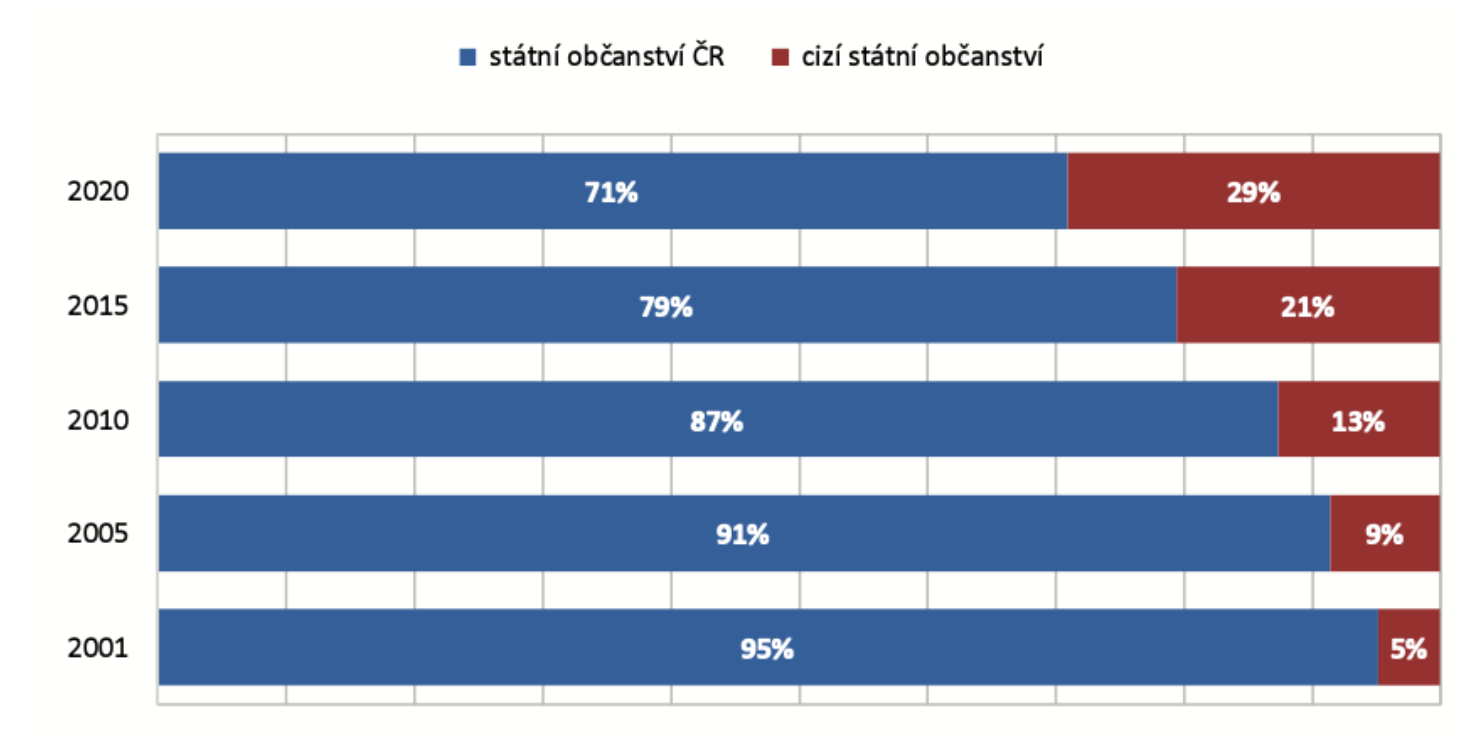
\includegraphics[width=16cm]{Maturitni Prace/images/obcanstvi_VS.png}
                    \caption[Rozložení studentů podle státního občanství 2001/20]{Rozložení studentů podle státního občanství mezi lety 2001 a 2020; Zdroj: ČSÚ/MŠMT}
                    \label{fig:obcanstvi_VS}
                \end{figure}
                Mezi nejčastější cizince studujících na~ ICT vysokých školách v ČR patří Slováci, kteří tvořili více než polovinu (3248 osob) zahraničních studentů na oboru ICT na~Českých vysokých školách. Další hodně zastoupení studenti jsou Rusové (17\%, 1081 osob), Ukrajinci (8\%, 535 osob) dále jsou to studenti z Kazachstánu, Běloruska, Kyrgyzstánu, Číny a~Spojených států amerických aj. Celkem v roce 2020 mělo na vysokých školách v Česku v ICT oborech alespoň jednoho studenta z~93 států.\cite{LidskeZdrojeVIT}
                
                \begin{figure}[h]
                    \centering
                      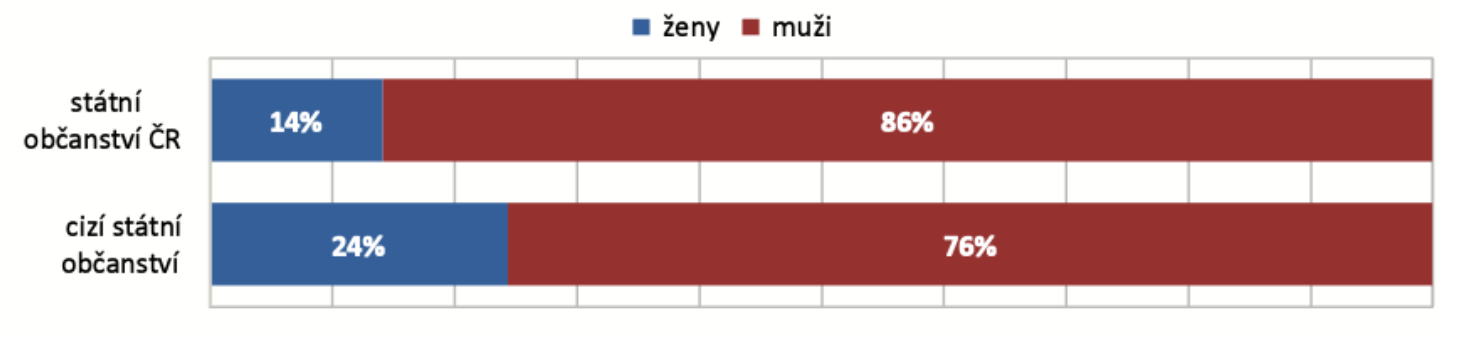
\includegraphics[width=16cm]{Maturitni Prace/images/obcanstvi_a_pohlavi_VS.png}
                    \caption[Diverzita zahraničních studentů ICT vysokých škol v roce 2020 v ČR]{Diverzita zahraničních studentů ICT vysokých škol v roce 2020 v ČR; Zdroj: ČSÚ/MŠMT}
                    \label{fig:obcanstvi_a_pohlavi_VS}
                \end{figure}
                
                Zajímavostí na zahraničních studentech je, že skoro čtvrtina jsou ženy a to i přesto, že se jedná o ICT obory.~\cite{LidskeZdrojeVIT}
               
                 
               
                
            \subsection{Věkové rozložení studentů ICT oborů na vysokých školách v České republice}
        
                Největší zastoupení studentů ICT oborů pokrývá věková kategorie 20-24 let, jedná se o dvě třetiny celkových studentů ICT oboru (obr.: \ref{fig:vek_VS}). Většina těchto studentů šla na vysokou školu rovnou po ukončení středoškolského studia. Další hodně zastoupenou věkovou skupinou jsou osoby ve věku 25-29 let, což je běžný věk pro studenta vysoké školy, převážně doktorského studia. Zajímavostí jsou ale studenti mladší 20 let. V roce 2020 jejich počet přesáhl hranici 2500. Nejvíce, přes 2000 je v této kategorii devatenáctiletých, zároveň ale na vysokých školách na~ICT oboru studuje přibližně 200 osmnáctiletých a 30 sedmnáctiletých studentů. Vzhledem k tomu, že věk českého maturanta se pohybuje nejčastěji mezi 19 a 20 roky, nebude překvapením, že nejmladšími studenty byly v roce 2020, až na 11 osmnáctiletých, cizinci, jelikož zde školu dokončují v nižším věku.~\cite{LidskeZdrojeVIT}
                 
                 \begin{figure}
                    \centering
                     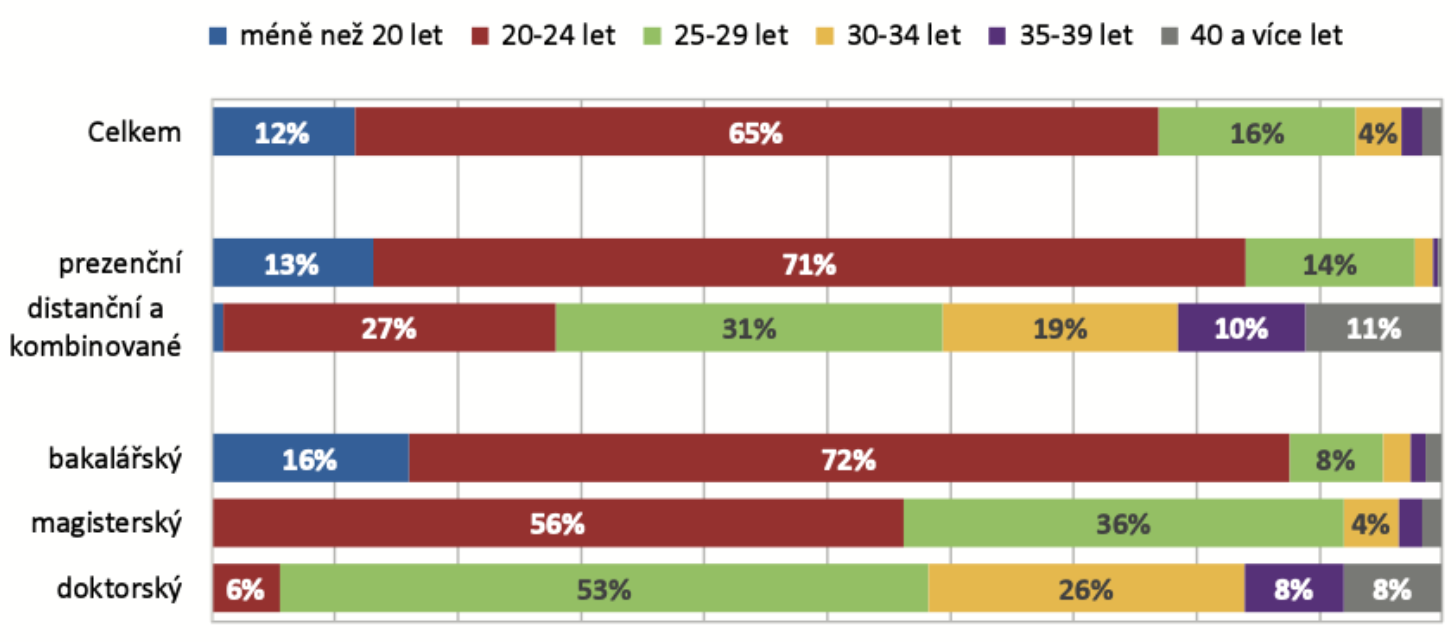
\includegraphics[width=16cm]{Maturitni Prace/images/vek_VS.png} 
                     \caption[Rozdělení studentů podle věku na VŠ v roce 2020 v ČR]{Rozdělení studentů podle věku studentů na vysokých školách v roce 2020 v ČR; Zdroj: ČSÚ/MŠMT}
                     \label{fig:vek_VS}
                 \end{figure}
                
                V grafu jsou dobře vidět patrné rozdíly ve věkové struktuře studentů v jednotlivých formách studia a různých studijních programech. Zajímavé je, že s věkem roste také zájem o distanční a~kombinované  studium. Prezenční formu studia upřednostňují věkové kategorie 20-24 let. Naopak distanční a kombinované studium upřednostňují kategorie starší 25 let. Důvodem může být kombinování vyššího studijního programu se~zaměstnáním. Nemělo by být ani překvapením, že bakalářský program je nejhojněji zastoupen mladými lidmi a doktorské vzdělání je vzhledem k rostoucímu věku během studia zastoupeno staršími studenty.~\cite{LidskeZdrojeVIT}
            
            %\subsection {Porovnání studentů ICT oborů na vysokých školách v České republice podle trvalého bydliště}
            
            %Nikoho nepřekvapí, že nejvíce studentů bydlí v Praze, v roce 2020 tomu bylo více jak 2500 vysokoškolských studentů ICT odborů. Dále to byli obyvatelé Středočeského a Moravskoslezského kraje, odkud dohromady studovalo přibližně 2000 studentů v tomto oboru. Naopak v Karlovarském kraji, nejmenším v České republice, je studium ICT oborů nejméně populární.~\cite{LidskeZdrojeVIT}
            %U starších studentů se ale data změní. V grafu můžete vyčíst, že starší studenti informatických oborů pochází hlavně z Prahy, ale také z Královéhradeckého a Moravskoslezského kraje, Středočeský kraj je tentokrát až za první polovinou s 1,5\% z celkové populace osob ve věkové kategorii 25-29 let.~\cite{LidskeZdrojeVIT}
            
            %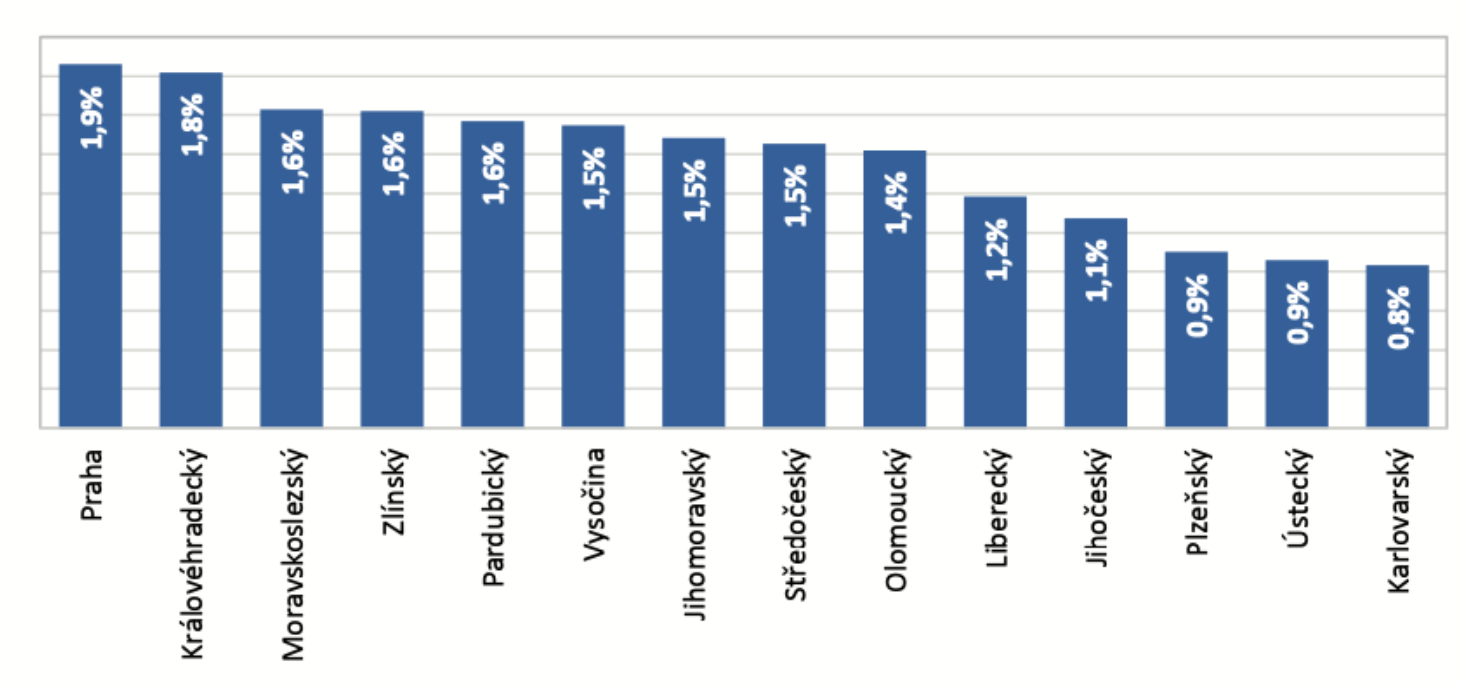
\includegraphics[width=16cm]{Maturitni Prace/images/kraje_VS.png}  
            
    	    %\subsection{Studenti ICT oborů na vysokých školách v České republice v porovnání s EU}
                %porovnání ČR a~EU
            
            %Evropská unie je momentálně složená z 27 států, z nichž všechny poskytují možnost studia ICT oborů. V mezinárodním srovnání počtu studentů těchto oborů na vysokých školách si na tom Česká republika nevede úplně nejhůře. Nejlépe jsou na tom státy Rumunsko, Řecko,Švédsko , Bulharsko a Estonsko, kde procentuální podíl dívek na ICT vysokých školách je skoro 30\%. Česká republika pak dosahuje hodnoty 16\% dívek na Vš, což je pod celkovým průměrem 27 států EU. Tento průměr se dostal vyšplhal skoro až k 20\% dívek na vysokých školách zaměřených na ICT.~\cite{EmployedICTSpecialstBySex}
            
            %\begin{figure}                 
                %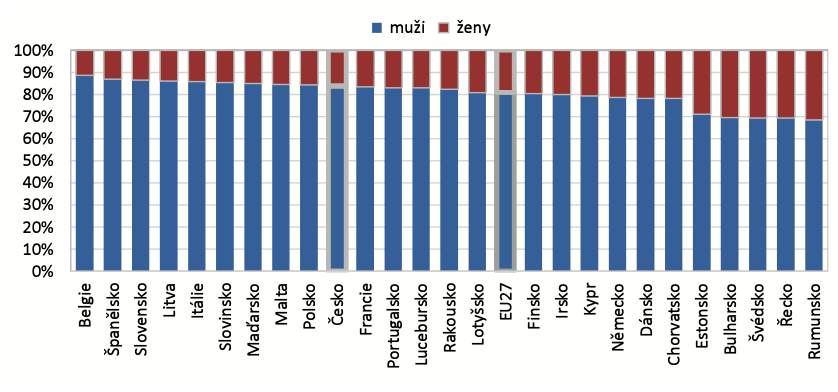
\includegraphics[width=16cm]{Maturitni Prace/images/studenti_ICT_mzn.png}
                %\caption{Zdroj: Eurostat}
            %\end{figure}
    
    	\section{Pracovní pozice v ICT v České republice}
            %pracovní pozice 
            % co ovlivňuje zaměstnanost nejen žen (věk/dosžené vzdělání/apod.)
            \begin{figure}[h]
                \centering
                 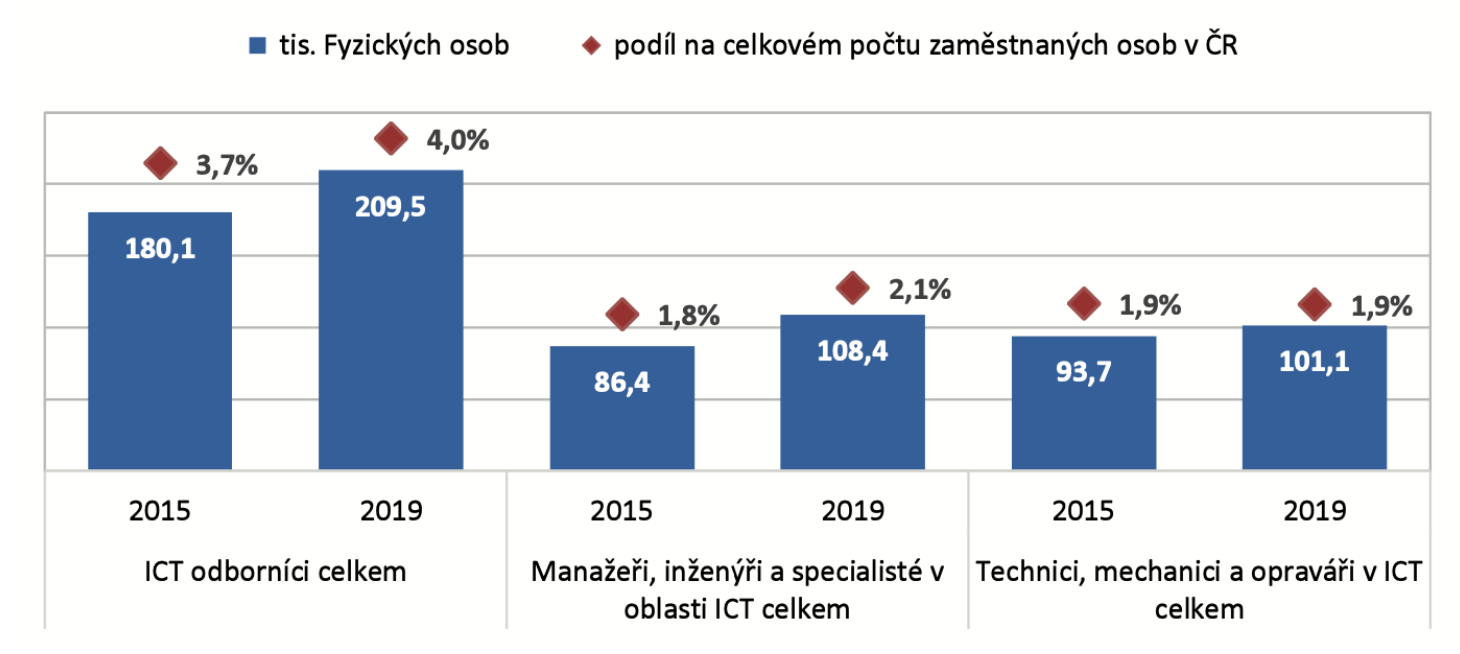
\includegraphics[width=16cm]{Maturitni Prace/images/odbornici_pocet.png}  
                 \caption[Rozdělení ICT zaměstnanců podle zaměření 2015/19]{Rozdělení ICT zaměstnanců podle zaměření 2015/19; Zdroj: ČSÚ}
                 \label{fig:odbornici_pocet}
            \end{figure}
            
            V roce 2019 bylo v České republice na pozicích ICT odborníka zaměstnáno skoro 210 tisíc osob, v celkové zaměstnané populaci se jedná o 4\% (obr.: \ref{fig:odbornici_pocet}). Pro porovnání máme data z roku 2015, kdy bylo zaměstnáno na těchto pozicích pouze 180 tisíc osob, což tou dobou tvořilo 3,7\% zaměstnanců. Odborníky ICT můžeme rozdělit na dvě skupiny, do první patří - Manažeři, inženýři a specialisté v oblasti ICT a do druhé - Technici, mechanici a opraváři v ICT celkem.Z grafu (obr.: \ref{fig:odbornici_pocet}) můžeme vyčíst, že procentuální rozdíl mezi lety 2015 a 2019 není markantní, když se ale podíváme na samotné hodnoty, zde jsou rozdíly trochu větší. Rozdíl u první skupiny je něco málo okolo 28 tisíc zaměstnanců, u druhé skupiny se jedná o 7 tisíc osob. Celkový rozdíl je mezi těmito roky roven skoro 30 tisícům ICT odborníkům. Za zajímavou statistiku považuji relativně vysoký počet zaměstnanců v tomto oboru. Z deseti dotázaných bylo 8 zaměstnanců, zbylá pětina pak OSVČ nebo podnikatelé.\cite{LidskeZdrojeVIT}
            
            \subsection{Vliv věku na zaměstnanost v ICT v České republice}
            %porovnání dotaženého věku na zaměstnanosti
                
                Pokud porovnáme data týkající se procentuální zaměstnanosti v tomto oboru v určitém věku, dostaneme se k níže uvedenému grafu (obr.: \ref{fig:odbornici_vek}). Jako nejpopulárnější volba pro práci v roce 2019 v tomto oboru je věkové rozpětí 30-39 let, v tomto věku se v ICT oboru nechalo zaměstnat až 6\% celkových zaměstnanců. Důvodem pravděpodobně je fakt, že se tato generace narodila do doby největšího vývoje technologie a rozšíření dostupnosti internetu, bylo pro ně tedy jednodušší se situaci přizpůsobit a naučit se s technologiemi pracovat. Za potvrzení této domněnky bych považovala i fakt, že věková kategorie 20-29let dosáhla v tomto odvětví celkové zaměstnanosti 5,1\%. ~\cite{InternetMadePublic}
                
                \begin{figure}[h]
                    \centering
                     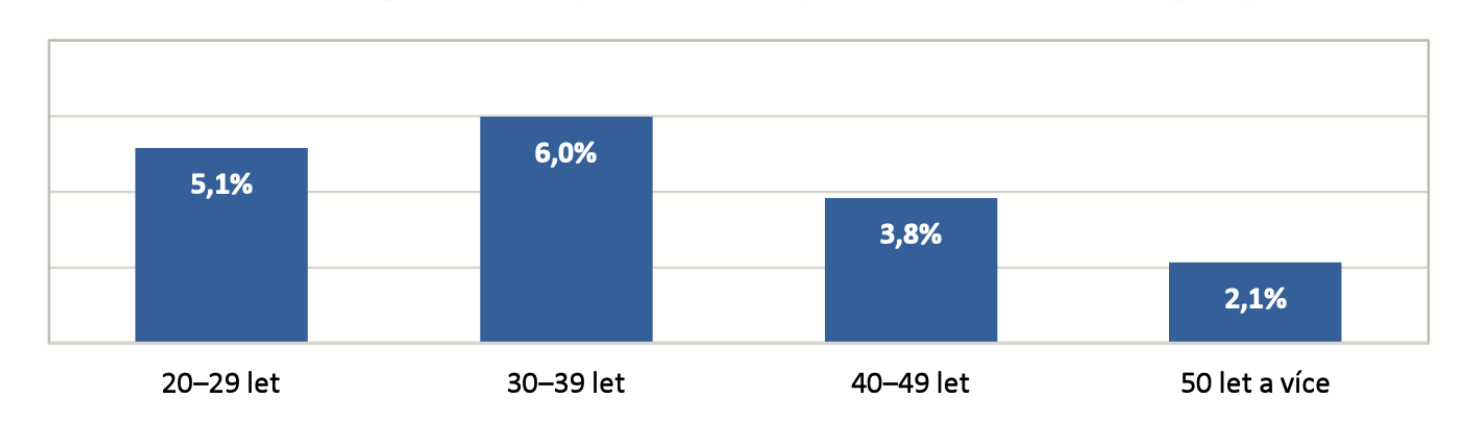
\includegraphics[width=16cm]{Maturitni Prace/images/odbornici_vek.png}  
                     \caption[Procento zaměstnanců v jednotlivých věkových skupin v ICT v ČR 2019]{Procento zaměstnanců v jednotlivých věkových skupin v ICT v roce 2019 v ČR; Zdroj: ČSÚ}
                     \label{fig:odbornici_vek}
                \end{figure}
                
                Obecně můžeme z dat roku 2019 (obr.: \ref{fig:odbornici_zamestnani_vek}) prohlásit že je toto odvětví populárnější spíše mezi mladými lidmi~do 39 let věku. Při rozdělení všech ICT odborníků na specialisty a techniky můžeme pozorovat 8\% rozdíl~u nejmladší zkoumané skupiny. Ten~je zdůvodněn větším požadavkem~na dokončení studia ve skupině ICT specialistů.~\cite{LidskeZdrojeVIT}
                
                \begin{figure}[h]
                    \centering
                     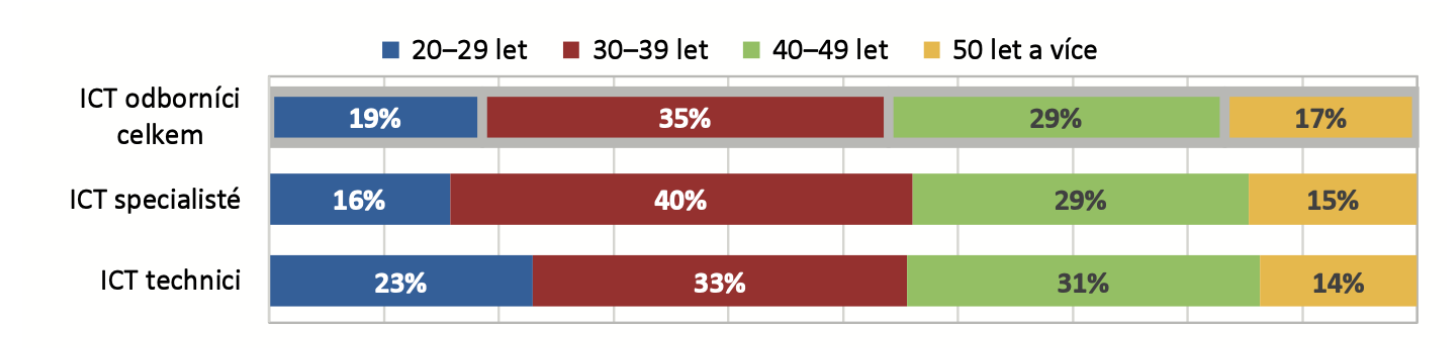
\includegraphics[width=16cm]{Maturitni Prace/images/odbornici_zamestnani_vek.png} 
                     \caption[Počet odborníků v ICT a jejich rozdělení v roce 2019 v ČR]{Počet odborníků v ICT a jejich rozložení na skupiny v roce 2019 v ČR; Zdroj: ČSÚ}
                     \label{fig:odbornici_zamestnani_vek}
                \end{figure}
        
            \subsection{Vliv nejvyššího dosaženého vzdělání na zaměstnanost v ICT v České republice}
            %porovnání dotaženého věku na zaměstnanosti
                
                ICT odborníky opět porovnáme ve dvou skupinách, jako tomu bylo v předchozí kapitole. Co se týká ICT specialistů  je zde vidět (obr.: \ref{fig:odbornici_vzdelani}) výše zmiňovaný důraz na dokončení studia jelikož 81\% dokončilo alespoň bakalářské či vyšší odborné studium. Z nichž více než dvě třetiny dokončili doktorské anebo magisterské studium, celkem to je 65\% ICT specialistů. Když se naopak podíváme na data ohledně ICT techniků, je zde vidět přesně opačný trend. Nejvíce zastoupenou skupinou jsou zaměstnanci jen s dokončenou střední školou s maturitou jedná se o 63\% ze všech ICT techniků. Když už se ale v tomto směru rozhodnou lidé studovat spíše dosáhnou až doktorského anebo magisterského studia, to se dá z dat říct obecně i o všech ICT odbornících. Za důvod této statistiky považuji dostatečný plat i přes níže dosažené vzdělání nebo vzdělávání mimo školský systém, tedy přes jiné kurzy, které mohou být úzce specializované na požadavky přímo na určitou pracovní pozici.\cite{LidskeZdrojeVIT}
                
                \begin{figure}[h]
                    \centering
                     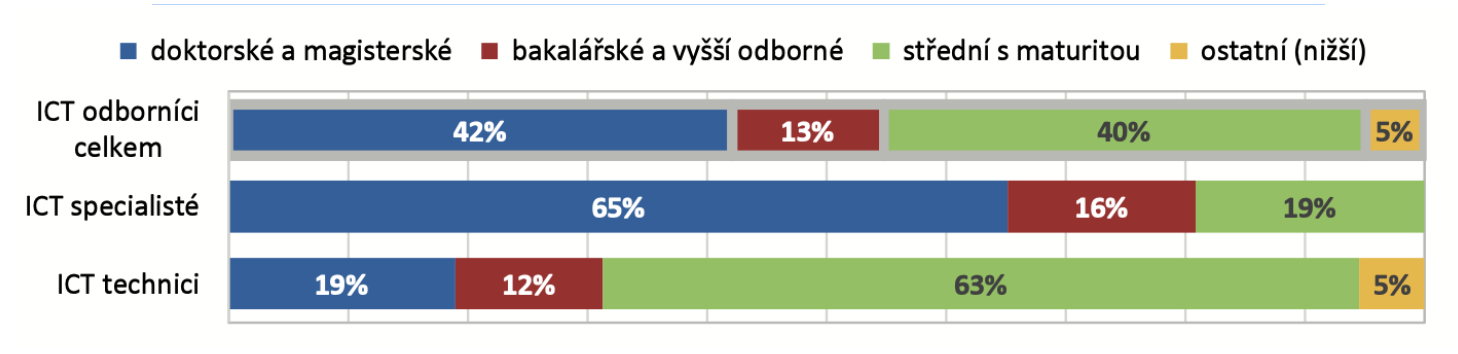
\includegraphics[width=16cm]{Maturitni Prace/images/odbornici_vzdelani.png}  
                     \caption[Rozložení zaměstnaných ICT odborníků - nejvyšší dosažené vzdělání 2019]{Rozložení zaměstnaných ICT odborníků a jejich nejvyšší dosažené vzdělání v roce 2019; Zdroj: ČSÚ}
                     \label{fig:odbornici_vzdelani}
                \end{figure}
  
            \subsection{Vliv pohlaví na zaměstnanost v ICT v České republice}
                Když se podíváme do roku 2004, byla v ICT odvětví více jak čtvrtina dívek. V roce 2006 se dokonce statistika dostala až ke 30\%. Od té doby se situace nezměnila a číslo nám stále klesá. Do roku 2010 byl pokles pozvolný, mezi lety 2010 a 2011 je velký pokles o 10\%, který ale koreluje s celkovým poklesem zaměstnanců v tomto odvětví. V roce 2011 situace na 10,7\% od té doby situace více méně klesá. V roce 2021 byla statistika obdobná 10\%, na jednu stranu je dobře, že procento neklesá, ale zároveň by se situace měla začít více řešit, jelikož právě minulost nám ukazuje, že ženy do ICT patřily a stále by patřit měly.\cite{EmployedICTSpecialstBySex}
                
  
        \section{Porovnání pracovních pozic s EU}
                \begin{figure}[h]
                    \centering
                    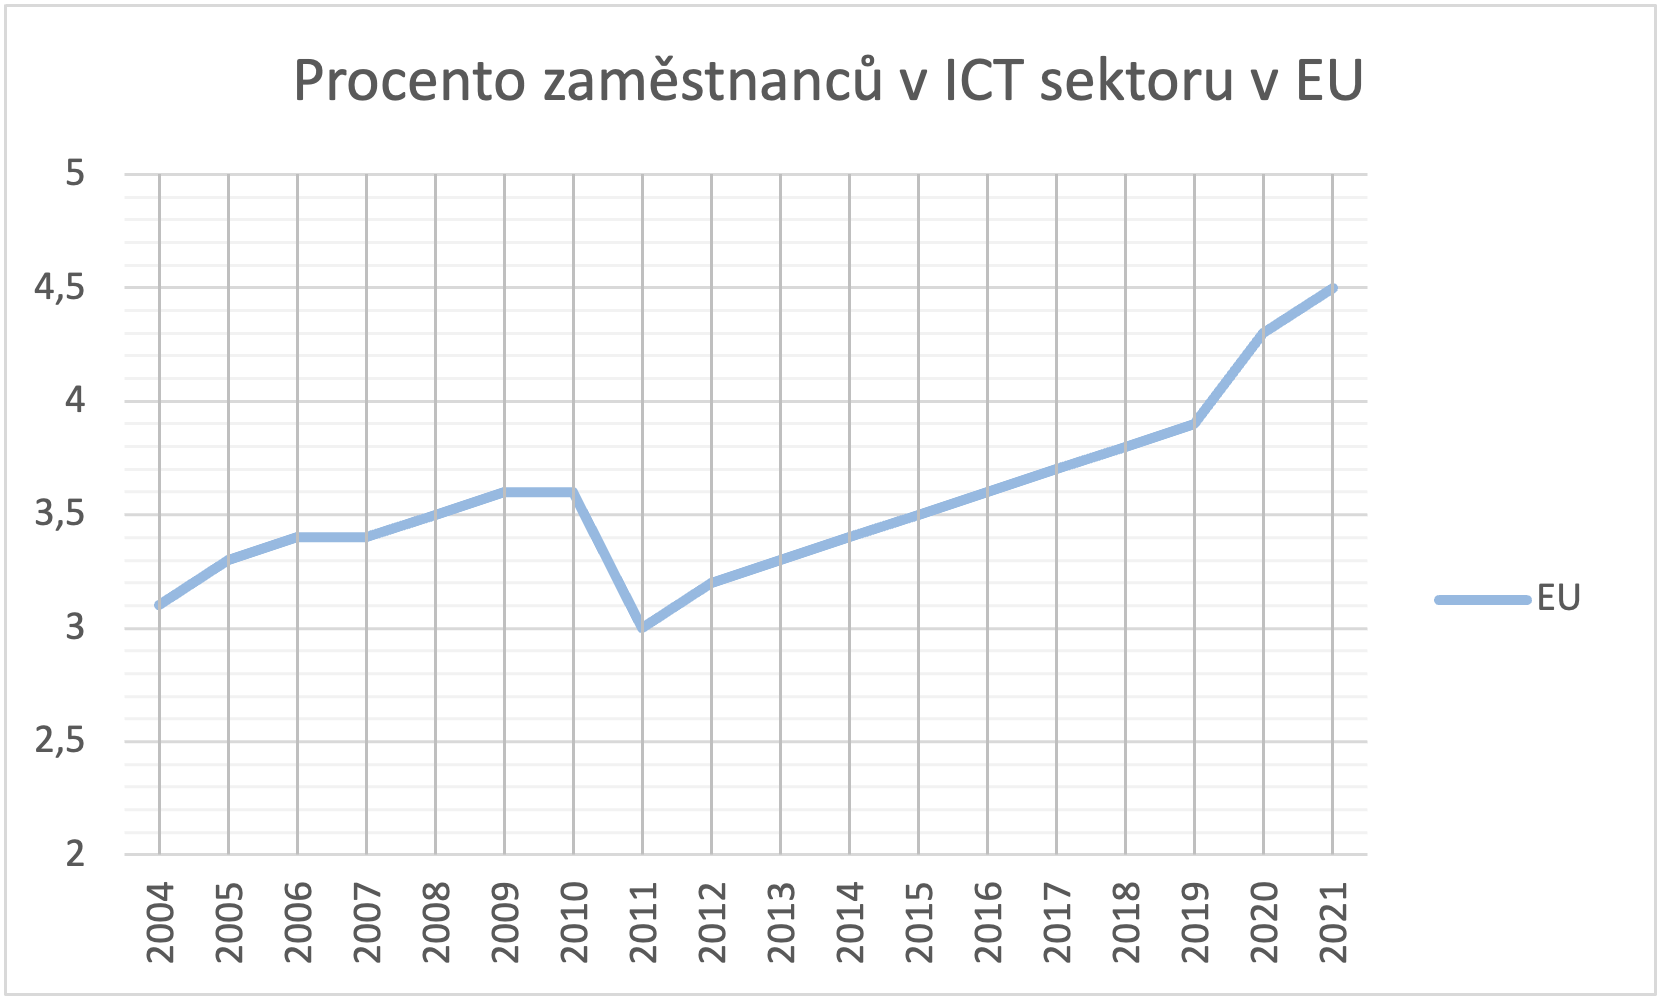
\includegraphics[width=16cm]{Maturitni Prace/images/odbornici_ICT_EU.png} 
                    \caption[Procento ICT odborníků v EU 2004/21]{Procento ICT odborníků v EU; Zdroj: Eurostat}
                    \label{fig:odbornici_ICT_EU}
                \end{figure}
                V posledních 10 letech v tomto odvětví nedošlo k žádnému velkému poklesu zaměstnanců (obr.: \ref{fig:odbornici_ICT_EU}). Počet zaměstnanců převážně rostl. Největší vliv na tuto situaci má neustálý nárůst dostupnosti připojení k internetu v domácnostech. Pro porovnání dostupnosti internetu můžeme využít data průměru Evropské Unie. V roce 2002, kdy máme nejstarší data, mělo přístup k internetu skoro 36\% domácností. Za 20 let se toto číslo vyšplhalo skoro až k hodnotě 93\%. To je průměrný nárůst o 2,85\% domácností ročně. Když to porovnáme s rokem 1993, kdy byla organizací CERN oficiálně spuštěna aktualizace, díky které byl internet dostupný pro širokou veřejnost \cite{InternetMadePublic}. Jde o nárůst z 0 na přibližně 93\% za 30 let. Zároveň je na grafu vidět velký pokles mezi lety 2010 a 2011.\cite{EmployedICTSpecialists-Total} \cite{HouseholdsInternetAccess}
                
            
            \subsection{Vliv věku na zaměstnanost v ICT v EU}
            
                Na grafu (obr.: \ref{fig:odbornici_ICT_EU_vek}) je vidět, že lidé v tomto odvětví spíše zůstávají, tak můžeme soudit podle většího podílu mladších zaměstnanců v levé části grafu. Naopak v bližší minulosti můžeme vidět větší nárůst u starších generací. Co se týká zájmu u mladších je spíše nižší než dříve, ale nemusí být tak markantní, jak ukazuje graf, jelikož právě zaměstnanci z minulých let, zestárli a dostali se do druhé zkoumané skupiny, čímž zvyšují její podíl. Ve skutečnosti tedy může být zájem stejný, jen počet zaměstnanců v celkovém odvětví může tento fakt zkreslovat. \cite{EmployedICTSpecialistsByAge}
                
                \begin{figure}[h]
                    \centering
                    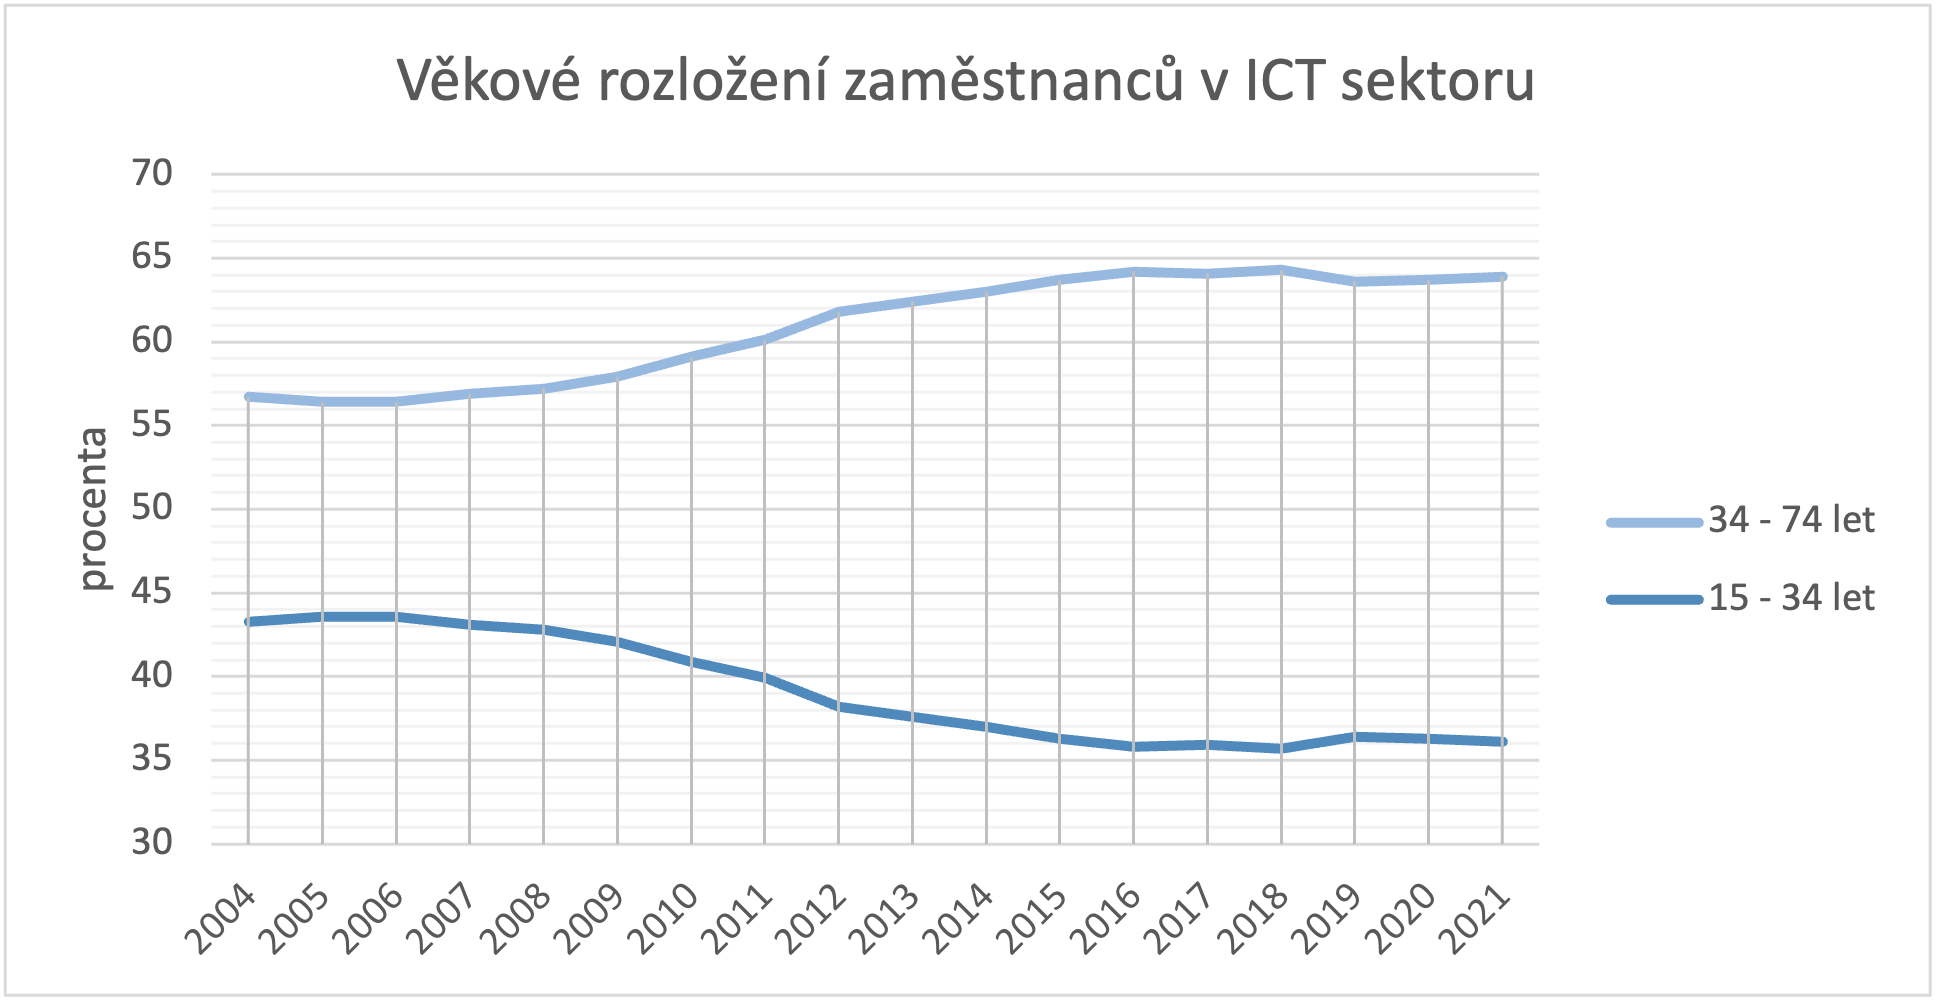
\includegraphics[width=16cm]{Maturitni Prace/images/odbornici_ICT_EU_vek.png} 
                    \caption[Procento ICT odborníků v EU podle věku 2004/21]{Procento ICT odborníků v EU podle věku; Zdroj: Eurostat}
                    \label{fig:odbornici_ICT_EU_vek}
                \end{figure}
                
            
            \subsection{Vliv nejvyššího dosaženého vzdělání na zaměstnanost v ICT v EU}
            %porovnání dosaženého vzdělání na zaměstnanosti EU
            
                Situace vyobrazená na grafu (obr.: \ref{fig:odbornici_ICT_EU_VZ}) nám ukazuje, že dříve zaměstnavatelé v EU nedbali na terciální vzdělání. Bylo tomu pravděpodobně, protože tou dobou školy v tomto odvětví neměli dostatečnou úroveň pro zaměstnavatele. Zároveň v roce 2021 je naopak velký nátlak na vysoké školy, jelikož 65\% zaměstnanců jsou právě ti s vysokoškolským.\cite{EmployedICTSpecialistsByEducationalAttainmentLevel}

                \begin{figure}[h]
                    \centering
                    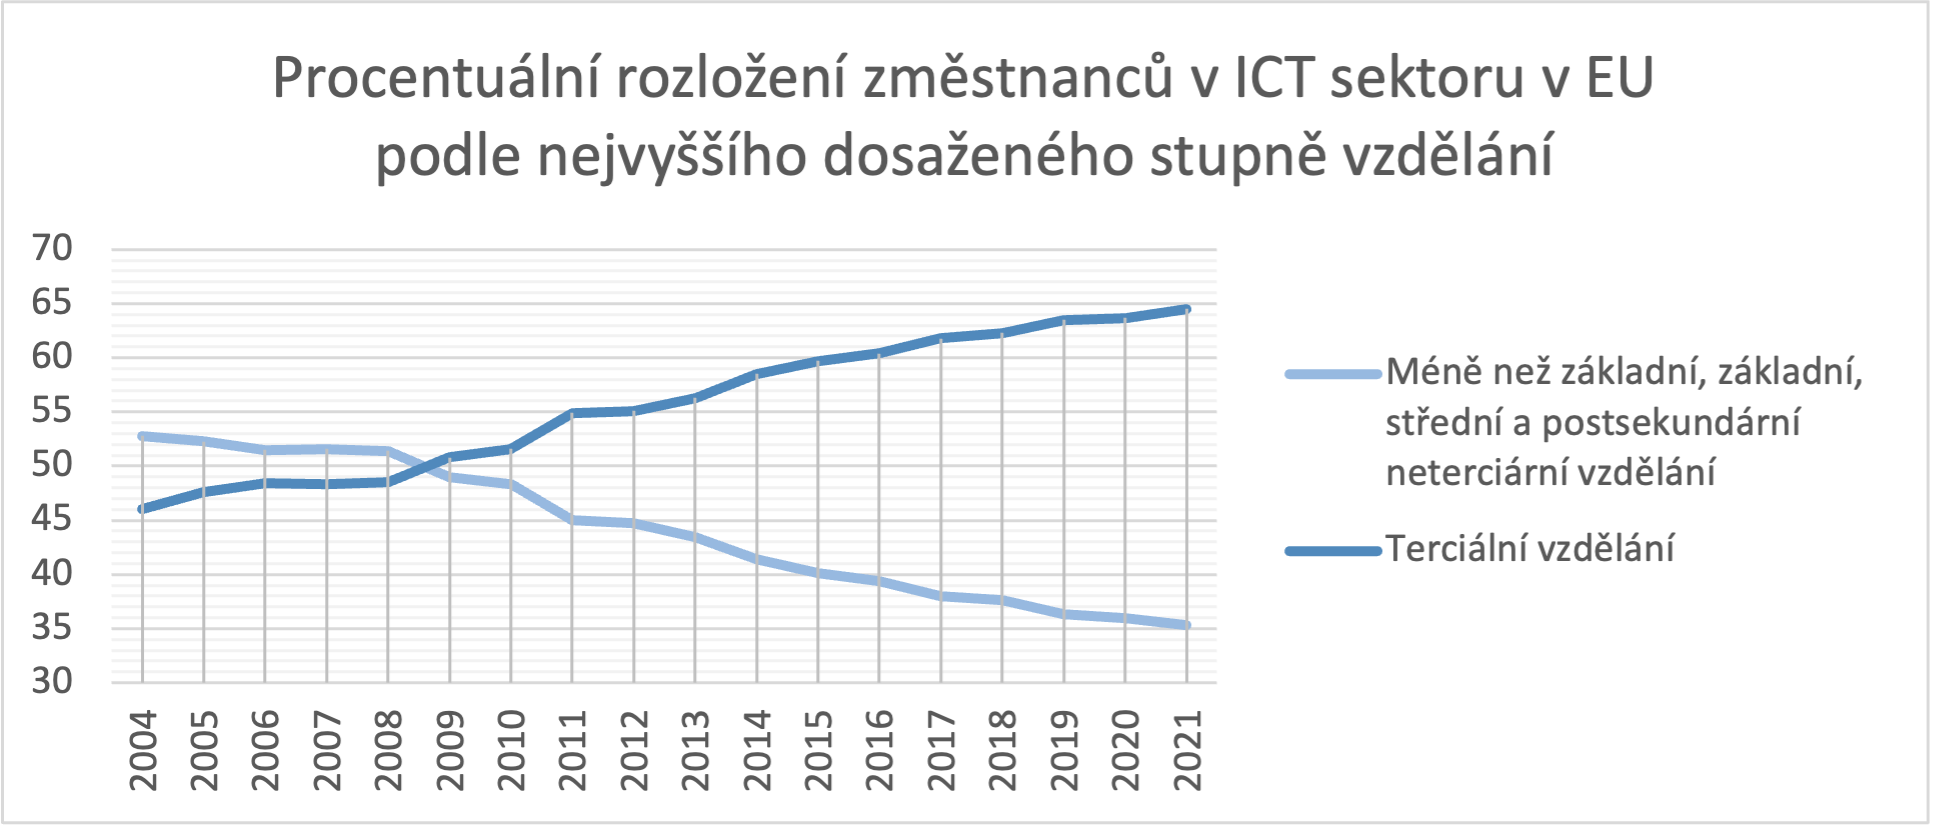
\includegraphics[width=16cm]{Maturitni Prace/images/odbornici_ICT_EU_VZ.png} 
                    \caption[Procento ICT odborníků v EU podle nejvyššího dosaženého studia 2004/21]{Procento ICT odborníků v EU podle nejvyššího dosaženého studia 2004/21; Zdroj: Eurostat}
                    \label{fig:odbornici_ICT_EU_VZ}
                \end{figure}
            
        	\subsection{Vliv pohlaví na zaměstnanost v ICT v EU}
                %porovnání ČR a~EU
                Když se zaměříme na pohlaví v tomto odvětví, nikoho nepřekvapí, že většina zaměstnanců budou muži (obr.: \ref{fig:odbornici_ICT_EU_pohlavi}). V minulosti se v tomto období pohybovalo přibližně 22\% žen a to i přesto, že tento směr nebyl tolik zajímavý. V roce 2010 je vidět pokles, který koreluje s celkovým poklesem zaměstnanců v tomto směru. Nebýt tomuto poklesu byl by trend situace stále rostoucí. V roce 2021 se procenta žen blíží k 20\% za pár lety se tedy můžeme dostat na stejnou hodnotu jako tomu bylo před 19 lety. Je důležité ale uvažovat, že počet žen může být i přes klesající procenta stejný nebo vyšší než v minulosti. \cite{EmployedICTSpecialstBySex}
                \begin{figure}[h]
                    \centering
                    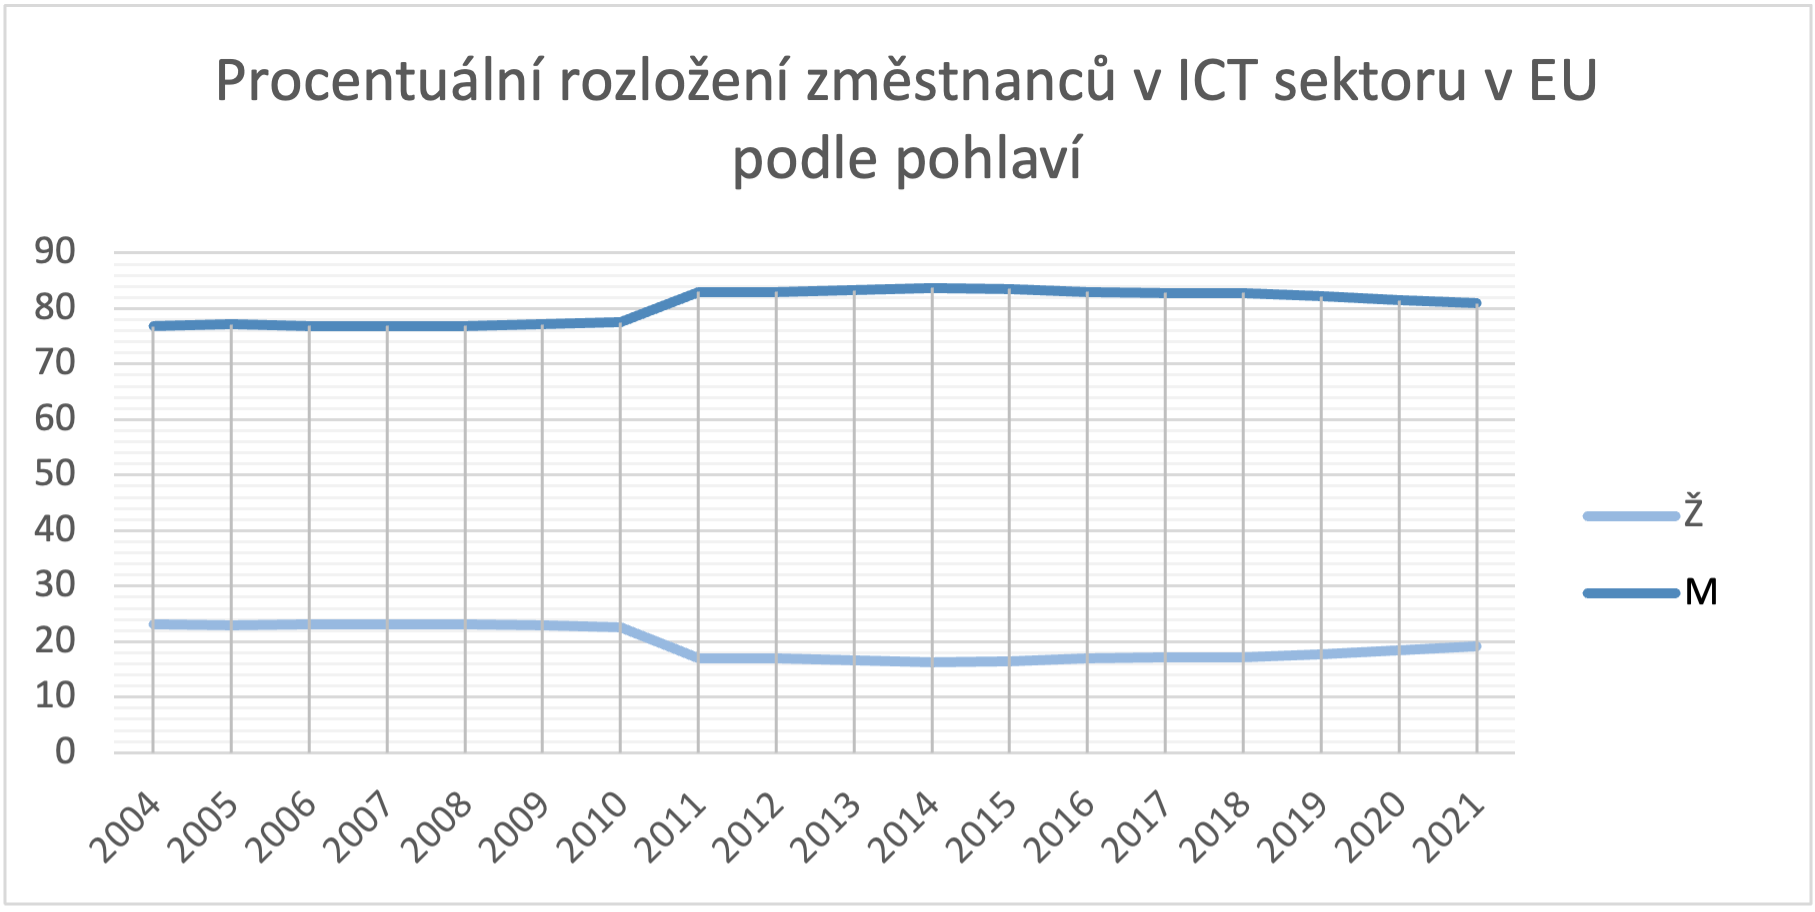
\includegraphics[width=16cm]{Maturitni Prace/images/odbornici_ICT_EU_pohlavi.png} 
                    \caption[Procento ICT odborníků v EU podle pohlaví 2004/21]{Procento ICT odborníků v EU podle pohlaví 2004/21; Zdroj: Eurostat}
                    \label{fig:odbornici_ICT_EU_pohlavi}
                \end{figure}

    \chapter {Řešení diverzity a nedostatku zaměstnanců v oblasti ICT}
    	
    	    \section{Situace ve firmách}
             Situace v EU je problémová v malých, středních i velkých podnicích. Proto se situaci snaží řešit školením zaměstnanců nebo ICT odborníky najímají externě. To se ale nevyplatí ve všech situacích, ale malé či střední firmy nemusí mít finance na zaplacení nákladů pro školení zaměstnance. Vypovídají o tom data z roku 2019, kdy školení ICT odborníkům nabízelo 56\% velkých firem, ale pouze 23\% středních a jen 6\% malých firem. Což je vůbec nejméně v porovnání financování školení pro jiné zaměstnance.\cite{EmploymentOfICTSpecialists}
             
        \section {Neziskové organizace}
            Kromě přizpůsobení firem a náklonnosti k nabírání žen i na pozice zaměřené na ICT jsou další možností i neziskové organizace. Takových skupiny je více, některé globální jiné lokální, dlouhodobě jsou ale obě důležité. Je také důležité, aby měly jiné cílové skupiny, aby byly schopny zasáhnout co nejvíce dívek a žen nehledě na věk, národnostní skupinu, finanční situaci aj. Pro reprezentaci jsem zvolila právě jednu globální neziskovou organizaci Czechitas, protože jsem s nimi spolupracovala na praktické části a zároveň i spíše lokální organizaci wITches.
            
            \subsection {Czechitas}

                Czechitas je česká nezisková organizace, jejíž misí je inspirovat, vzdělávat a~uplatňovat nové talenty pro posílení diverzity a~konkurenceschopnosti v~IT. Pořádá kurzy pro ženy, jednodenní a~vícedenní, v~poslední době se zaměřuje i~na dlouhodobé kurzy nebo tzv. Digitální akademie\footnote{velmi intenzivní dlouhodobé kurzy}. Mezi témata kurzů patří například programování, datová analýza nebo tvorba webu. Z účastnic těchto kurzů je pak tvořena komunita žen věnující se tomuto oboru.\cite{CzechitasCoDelame} 

                Celý příběh neziskové organizace se začal psát v~roce 2013, kdy se Dita Přikrylová (dnes Formánková) společně se svými kolegy a~přáteli zorganizovala v~Brně jednodenní workshop tvorby webových aplikací pro ženy. Celý projekt byl zastřešen pod názvem Rail Girls.\cite{CzechitasRailGirls}

                Po třech letech své existence Czechitas zvítězila v~Social Impact Award v~roce 2015, inkubátoru, do kterého se zapojily i~nynějšími členky správní rady Monika Ptáčníková a~Mirka Zatloukalová. Myšlenka brzy přilákala silnou komunitu předních IT specialistů, odborníků, firem a~dobrovolníků a~dala vzniknout celému portfoliu vzdělávacích aktivit.\cite{CzechitasSocialImpactAward}

                Již v~této době si lidé v~Czechitas uvědomovali důležitost rozhodnutí o~budoucí kariéře, a~proto za podpory Microsoftu spustili týdenní letní školu ve spolupráci ČVUT v~Praze, jejímž cílem bylo inspirovat středoškolačky ke studiu IT.\cite{CzechitasLetniSkola}
    
                V~roce 2016 nezisková organizace získala důvěru a~podporu Google a~to jako první iniciativa ve střední Evropě. Na~základě toho se skupina začala věnovat tvorbě prvního rekvalifikačního kurzu pro maminky na~mateřské dovolené - Digitální akademii. \cite{CzechitasGoogleGrant}

                \begin{quote}
                    \textit{``Cílem programu je vyjít vstříc pracovnímu trhu, protože státní vzdělávací systém nedokáže tak rychle reagovat na~změnu poptávky ze strany zaměstnavatelů,`` říká Dita Přikrylová, zakladatelka Czechitas.}\cite{CzechitasGoogleGrant}
                \end{quote}

                Velkým milníkem pak bylo září 2019, kdy se za podpory CTP pobočka v~Brně, jako první, přestěhovala do vzdělávací centra CTP Czechitas House.\cite{CzechitasHome}
                
                Dalším zlomovým okamžikem byl 12. březen 2020, kdy byl vyhlášen nouzový stav v~ČR.\cite{NouzovyStav} Během jednoho týdne organizace musela všechny jednodenní a~dlouhodobé kurzy i~celé Digitální akademie přesunout do online formy. Díky tomuto kroku se ale Czechitas mohla rozrůst i~do menších regionů a~být ještě dostupnější.\cite{Czechitas2020}

                V~roce 2021 organizace získala největší grant v~historii, 26 miliónu korun od dánského výrobce oken Velux.\cite{ForbesGrant}

                Na~přelomu roků 2021 a~2022 se Czechitas začali věnovat i~středoškolákům. Spustili několikaměsíční program pro studenty středních škol, který byl při řádné docházce zcela zdarma.\cite{CzechitasOvladniDigitalniTechnologie}
                
                V~létě 2022 se podařilo zrealizovat návaznou Letní školu IT 2 pro absolventky předchozích letních škol.\cite{Czechitas2022}


            \subsection {wITches}
                Tato nezisková organizace je složená ze studentek Fakulty elektrotechnické Českého vysokého učení technického v Praze. Cílovou skupinou této organizace jsou děti od 5. do 9. třídy základní školy, pro které pořádají workshopy zdarma. Ty jsou na témata: programování, elektrotechnika, robotika. 

                Programování se děti učí v prostředí SCRATCH, pokročilejší pak přejdou do programovacího jazyku PYTHON. Co se elektrotechniky týče, tak se děti její základy učí se stavebnicemi BOFFIN a MICRO:BIT. A pokud mají děti zájem o roboty mohou se začátky naučit díky LEGO nebo OZOBOT.
	
\part{Prezentace na školách}

        \section{Vize projektu}
    
            Celý projekt je organizován neziskovou organizací Czechitas, kde v~době psaní této práce působím jako ambasador, a~jedná se o~přednášky na~středních školách. Jelikož se obdobnému projektu Czechitas ještě nevěnovala, bylo potřeba si před začátkem definovat jeho vizi. Do projektu zapojeno více dívek a~každá z nás měla trochu jiná očekávání. Já ale vnímám tento projekt jako příležitost pro motivaci dívek na~středních školách k uvažování o~studiu na~vysoké škole s informatickým nebo technických zaměřením a~propagaci této neziskové organizace. Zároveň se projektem snažíme zasáhnout i~chlapce, aby změnili názor na~dívky, které se tímto směrem chtějí vydat. To je důvod proč třída není na~přednášku rozdělena. Je totiž potřeba měnit názory nejen dívkám, ale i~okolí, které ve výběru vysoké školy nebo i~budoucího zaměstnání hraje mnohdy velkou roli.
        
            Pro projekt byly vybrány prezentace, a~to přímo na~školách ve výuce v~hodinách informatiky, hlavním důvodem bylo zasažení všech studentů, hlavně těch, kteří by se na~obdobnou přednášku jinak nechtěli přihlásit. A~to ať z důvodu toho, že jim téma není blízké nebo, že by mimo výuku neměli čas, proto jsme se tomuto snažili předejít a~zaměřili se na~čas běžné výuky. 

            Cílovou skupinou pak byly 1.~a~2. ročníky středních škol a~jim odpovídající ročníky víceletých gymnázií, ale pokud měla škola zájem neměli jsme problém přednášku poskytnout i~starším studentům i mladším studentům.

        \section{Průběh}

            Přípravy projektu začaly už před letními prázdninami. Nejprve jsme se sešli s vedoucími projektu Kateřinou Jeřábkovou a~Markem Sedlákem v~pražské kanceláři Czechitas. Kde jsme následně plánovali samotnou prezentaci, aby byla pro studenty záživná a~měla spád. O~vizuální stránku se následně postaral marketingový tým Czechitas.

            \subsection{Moje prezentace}
                Každá z ambassadorek jsme obdržely základní prezentaci, kterou jsme si mohly upravit podle sebe, aby korespondovala s naší osobní vizí projektu. 
                Já jsem si svou prezentaci rozdělila na~tři hlavní části. 

                Úvodem prezentace bylo mé představení, uvedení do situace, proč jim přenáším právě já a~jak jsem se do také situace dostala. Hlavním účelem popsání mé cesty je přiblížení se studentům, aby si uvědomili, že jsem také byla v~situaci, jako oni a~dokázala jim, že je možné se již v~tomto věku profilovat a~to i~mimo školu.

                Následovalo, stejně jako v~této práci uvedení do problému. Důležité v~této části je porovnání dat s něčím, co je jim bližší, aby si hodnotu dokázali představit nebo alespoň porovnat. Tedy v~případě, kdy je jim předána informace ohledně nedostatku 30000 IT odborníků je nezbytné toto číslo doplnit například o~počet studentů, kteří v~posledním roce odmaturovali (přibližně 72 tis. \cite{PocetMaturantu}), aby posluchači měli alespoň nějakou představu, o~jak velké číslo se v~kontextu jedná. V~této části je také do prezentace zapojeno využití mobilních telefonů formou odpovídání anonymního dotazníku, a~to z důvodu využívání technologií při výuce a~zamezení mnou nekontrolovaného využití telefonu během přednášky. Při přednášce jsem očekávala, že bude přítomný i~pedagog, kterého by toto využití také mohlo inspirovat, to ale nemám nijak podložené, zda-li se tak po přednáškách stalo.

                Poslední část přednášky je téma bezpečnost. Nejprve se v~přednášce se studenty snažím zaujmout faktickými, ale trochu děsivými daty, jako např. \uv{Co se stane na~internetu každou minutou?}. Posluchače se pak snažím informovat o~metodách útočníků na~internetu - phishing, blackmailing, malware a~ransomware. A~opět zapojuji interaktivní činnost - phishingquiz.withgoogle.com, kde si mohou oni sami vyzkoušet, odhalení falešných emailů. Pár příkladů s nimi projdu sama, na zbytek se pak mohou podívat po přednášce (ale záleží přednáška od přednášky, někdy stihneme dodělat během). Při procházení jim popisuji, na~co si dát pozor a~průběžně se ptám, co by teď udělali. Žákům popisuji toto pořadí: Nejprve zkontroluji validitu e-mailu, zda jsem v~poslední době řešila nějakou situaci korelující s obsahem zprávy, dále zkontroluji odesílatele a~po najetí na~odkaz (či dlouhém stisku odkazu na~dotykovém telefonu) se v~levém dolním rohu zobrazí, kam web odkazuje. Teprve pak by na~odkaz měli kliknout. Mluvím také o~psychickém nátlaku jako např. pomocí času například situace \uv{Máte posledních 10 minut} apod..

        \subsection{Navštívené školy a~průběhy přednášek}
                Na celém projektu, jak již bylo výše zmíněno, pracujeme v týmu několika lidí, kde jsem se přednášek chopila spolu s dalšími 3 holkami. Dohromady jsme od září do prosince v roce 2022 navštívily 12 škol, kde proběhlo 26 přednášek. Celkem se nám tedy podařilo přednášku uspořádat přibližně pro 950 žáků. Z nichž nám 440 (cca 46\%) odpovědělo na dotazník na konci prezentace, díky kterému můžeme vyhodnotit vliv přednášek. Přednášky se konaly v Praze, Středočeském, Jihočeském kraji a na Moravě, přičemž každou oblast měla na starost jedna přednášející.  

                Vůbec první přednáška proběhla u nás na gymnáziu Jírovcova 8 v Českých Budějovicích. Jelikož do té doby jsme si zkoušely přednášky jen v kanceláři bylo zde hodně problémů. Za největší považuji problém se sli.do a špatně vygenerovaný QR kód na dotazník pro zpětnou vazbu. Situaci ohledně sli.do jsem vyřešila větším zapojením přímé interakce a odkaz na dotazník jsem poslala žákům po přednášce. Kvůli tomu jsem i obdržela méně odpovědí.

                Druhá přednáška probíhala na žádost ŠKODA AUTO a.s., dlouhodobého partnera neziskové organizace Czechitas, v Mladé Boleslavi na Gymnáziu Dr. Josefa Pekaře. Jelikož zde bylo více tříd rozhodly jsme se si přednášky rozdělit, abychom si vzájemně mohly předat zpětnou vazbu.

                Třetí škola, kterou jsem v rámci přednášek navštívila bylo soukromé Česko-anglické gymnázium v Českých Budějovicích. Přednášky zde proběhly dvě, pro dva první a dva druhé ročníky. Jelikož se mi ten den ráno rozbil počítač, tak opět nebylo možné využít službu Sli.do, ale v tomto případě to nebyl problém. Studenti v obou skupinách byli velmi komunikativní a nebáli se vyjádřit svůj názor a zapojit se do přednášek. 

                Poslední škola, kterou jsem navštívila s přednáškou byla Gymnázium Písek. Domluva se školou byla velmi špatná a teprve až na místě jsem se dozvěděla, že spojili dohromady několik tříd. Tedy přednášku, která byla plánována pro 30 maximálně 60 žáků, jsem přednášela pro přibližně 120 studentů. Bylo to velmi náročné nejen pro mě, tak i pro posluchače. Mým cílem při přednášce je navození přátelské atmosféry, aby se studenti nebáli ptát na dotazy, a to v tomto případě si troufám říct, bylo až skoro nemožné. Studentů ani nenapomáhala tato situace, jelikož se mezi třídami neznali a o to více se báli klást otázky.
            
                
        \section {Zhodnocení dopadu přednášek}
            Výsledky přednášek se dají velmi těžko sledovat, celkově jsme oslovili přibližně 950 studentů napříč celou Českou republikou. Z celkového počtu jsem přednášela přibližně pro 450 studentů, z nichž mi zpětnou vazbu skrze dotazník poskytlo 128 žáků, tedy přibližně 28\%. Počet odpovědí se odvíjel podle počtu žáků ve třídě, paradoxně, čím více žáků ve třídě bylo, tím méně jsem obdržela odpovědí. Až na pár problémů s vysokým počtem žáků ve třídě nebo nefungující aplikace proběhla praktická část v pořádku a odnesla jsem si z ní nejen výsledky dotazníků, které níže rozeberu.

            \subsection{Vliv přednášek na dívky}
                
                Hlavním cílem zpětné vazby bylo dozvědět se, jaký vliv měla přednáška na uvažování studentů o studiu informatiky následně na vysoké škole. Tyto hodnoty rozdělené podle proběhlých přednášek na jednotlivých školách jsem vyobrazila ve sloupcovém grafu (obr.: \ref{fig:divky_uvazovani}). Za velmi zajímavé považuji odpovědi u poslední, šesté, přednášky, kde začalo po jejím skončení uvažovat 6 dívek o tomto směru. 
                
                \begin{figure}[h]
                    \centering
                    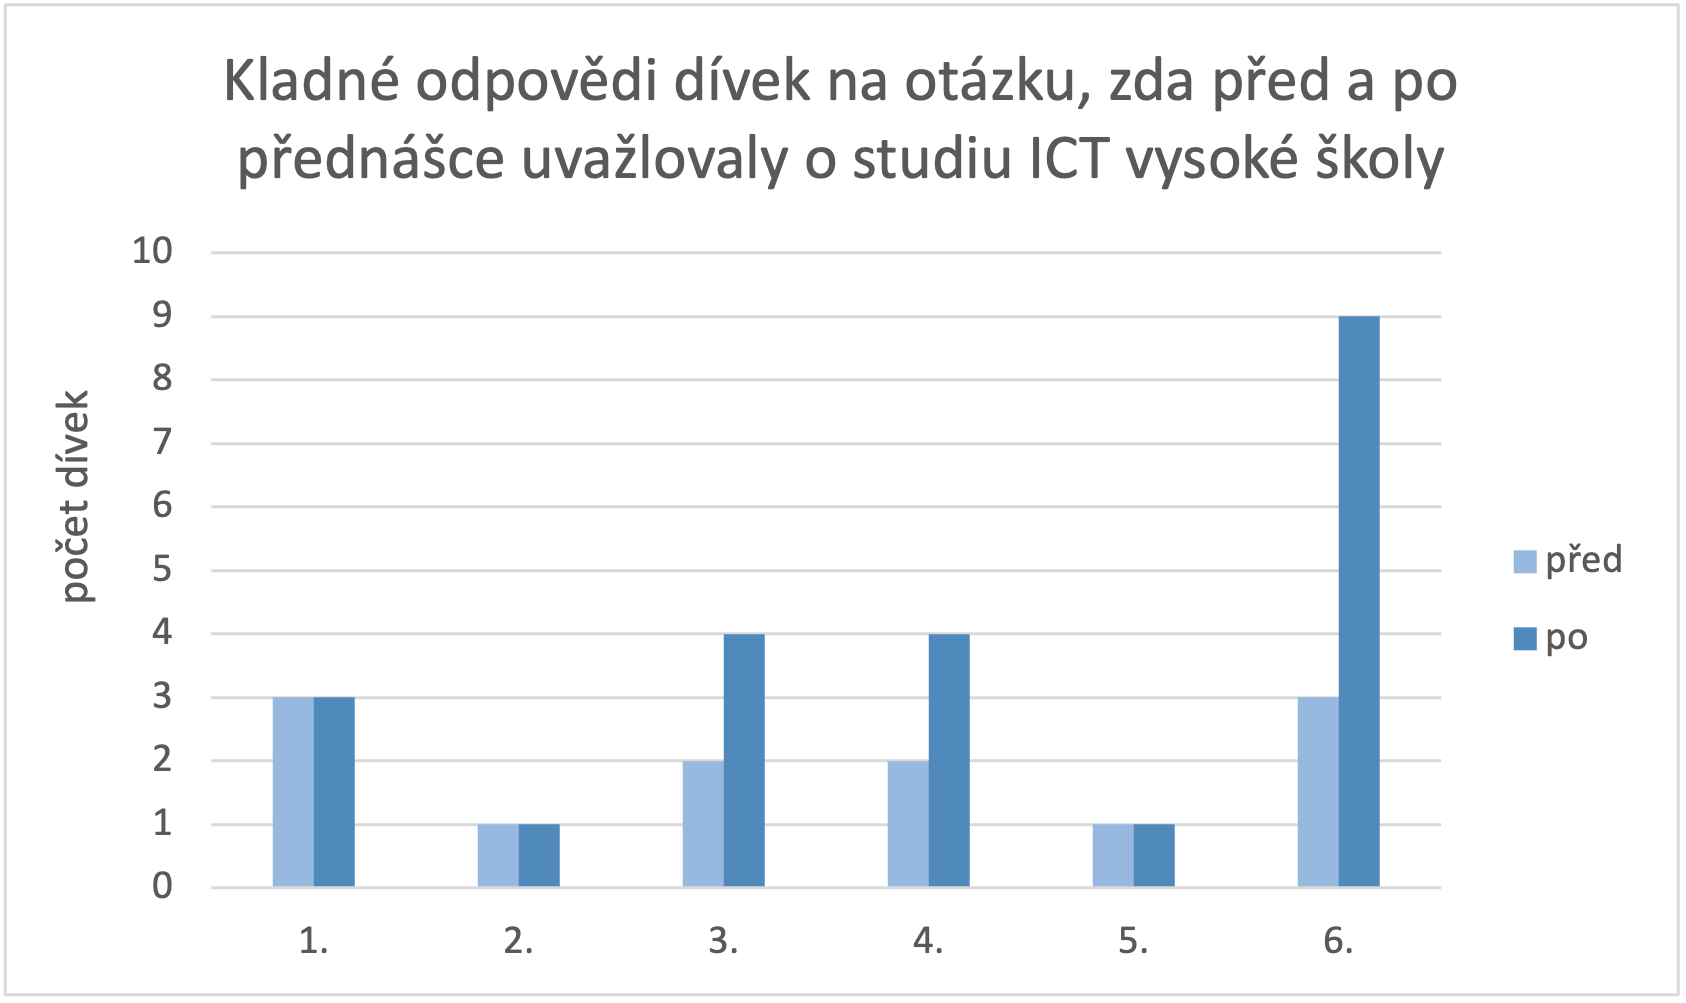
\includegraphics[width=16cm]{Maturitni Prace/images/divky_uvazovani.png} 
                    \caption{Počet kladných odpovědí od dívek na otázku, zda před a po přednášce uvažovaly o studiu na ICT VŠ}
                    \label{fig:divky_uvazovani}
                \end{figure} 
                
                Na těchto koláčových grafech (obr.: \ref{fig:divky}) jsou sečteny názory všech dívek ze všech přednášek před a po prezentaci. V tomto případě mám odpovědí jen přibližně 30\% ze všech přítomných studentů přednášek. Kdybychom tedy vycházeli z těchto dat, kdy přednáškou bylo ovlivněno 10 dívek, tak je zde možnost, že po mnou prezentovaných přednáškách jsem mohlo reálně o studiu informatické vysoké školy uvažovat 33 dívek. 
                 Jelikož přednášky probíhaly pro první a druhý ročník data nám i ukázala v jakém ročníku dívky více změnily názor. V mém případě to na plné čáře vyhrál druhý ročník, kde přednáška ovlivnila 8 ze všech 10 dívek (obr.: \ref{fig:prvak_druhak}). 
                \begin{figure}
                    \centering
                    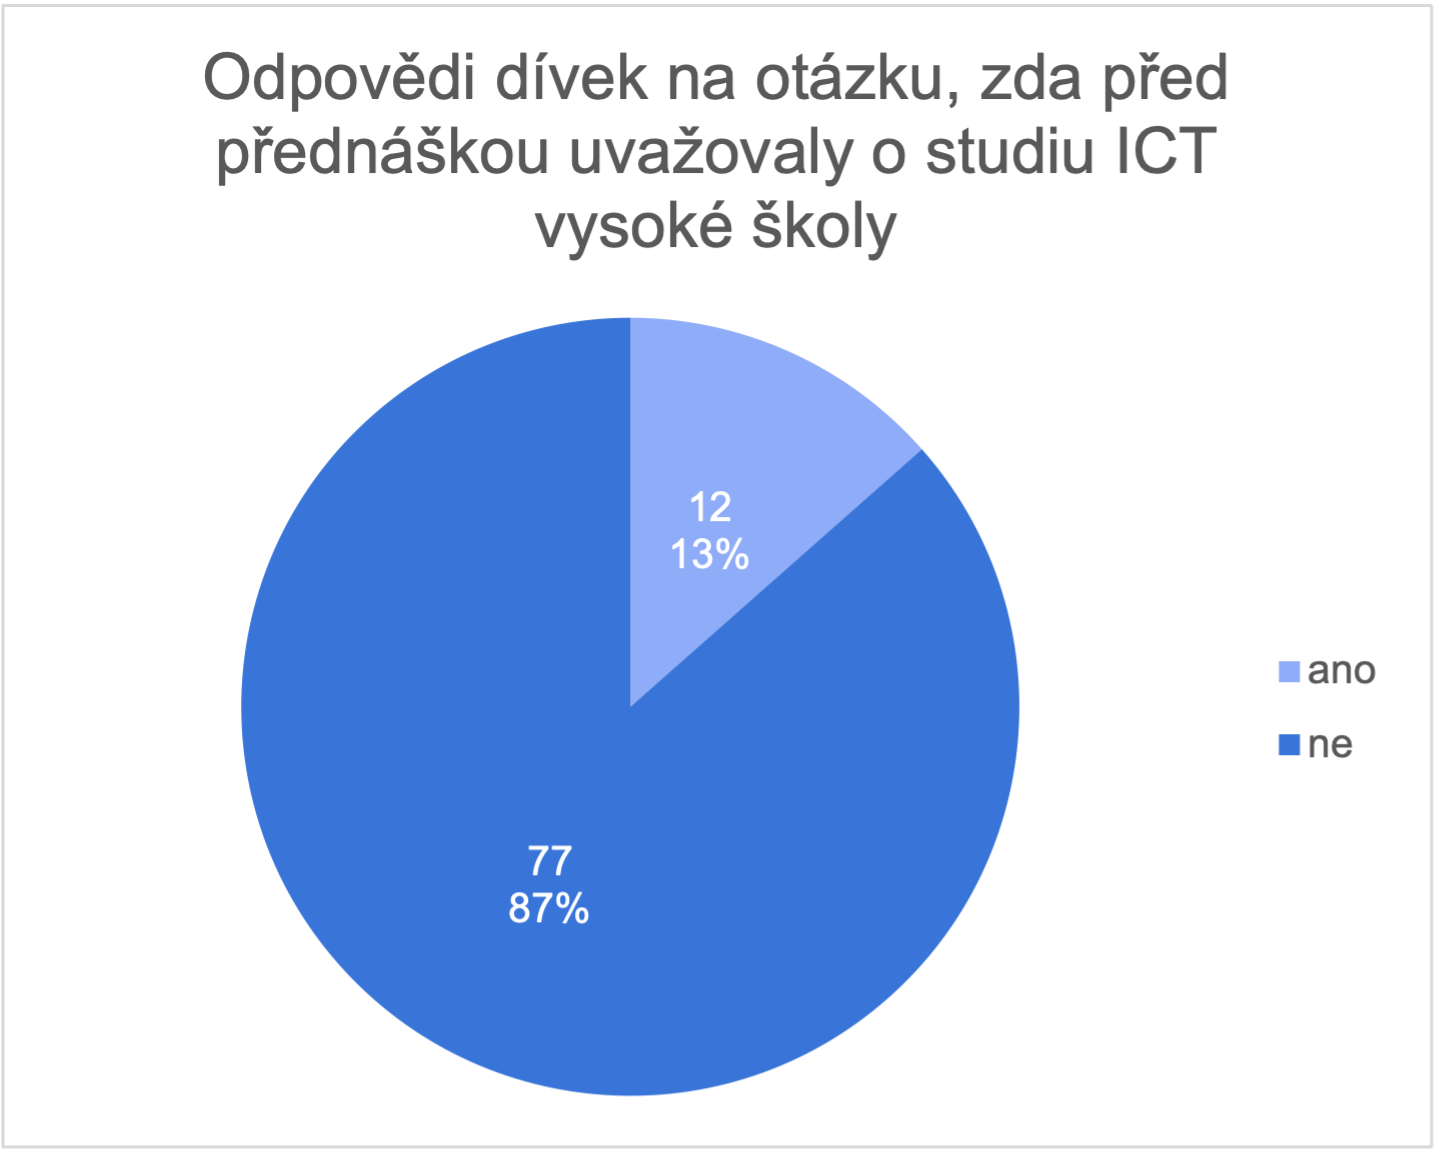
\includegraphics[width=8cm]{Maturitni Prace/images/divky_pred.png} 
                    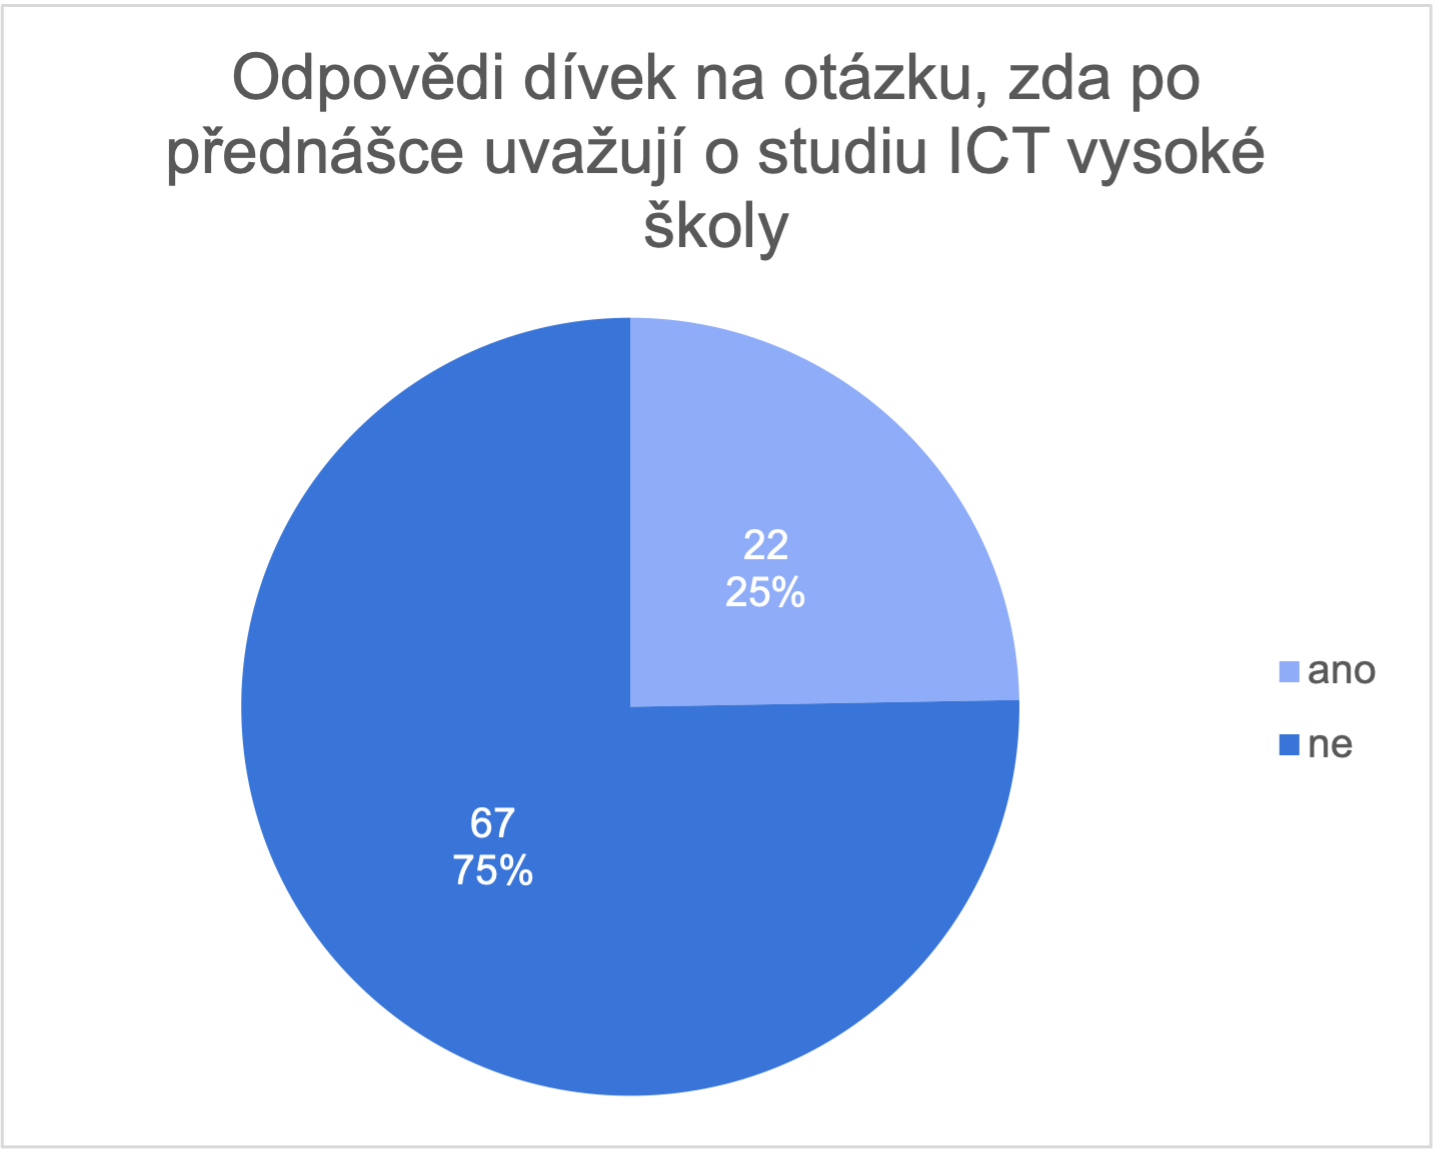
\includegraphics[width=8cm]{Maturitni Prace/images/divky_po.png} 
                    \caption{Odpovědi od dívek před a po provedených přednáškách na otázku zda uvažují o studiu na ICT VŠ}
                    \label{fig:divky}
                \end{figure}  
                
                \begin{figure}[h]
                    \centering
                    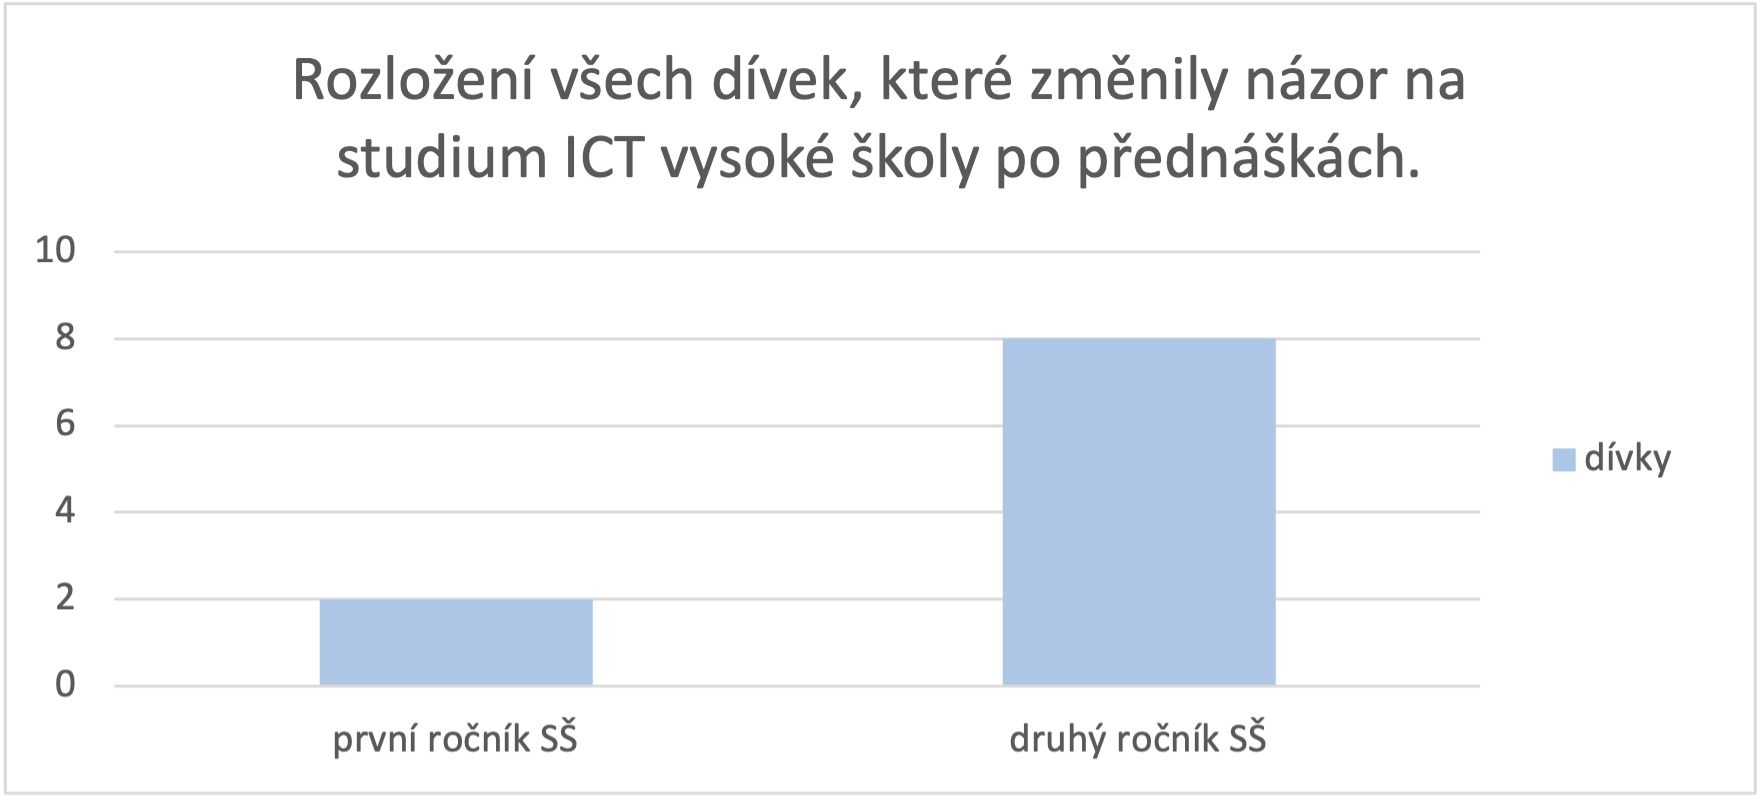
\includegraphics[width=16cm]{Maturitni Prace/images/divky_prvakXdruhak.png} 
                    \caption{Rozložení všech dívek, které po přednáškách změnily názor na studium ICT VŠ }
                    \label{fig:prvak_druhak}
                \end{figure}  
        
        
           \subsection{Vliv přednášek na chlapce} 
                
                \begin{figure}
                    \centering
                    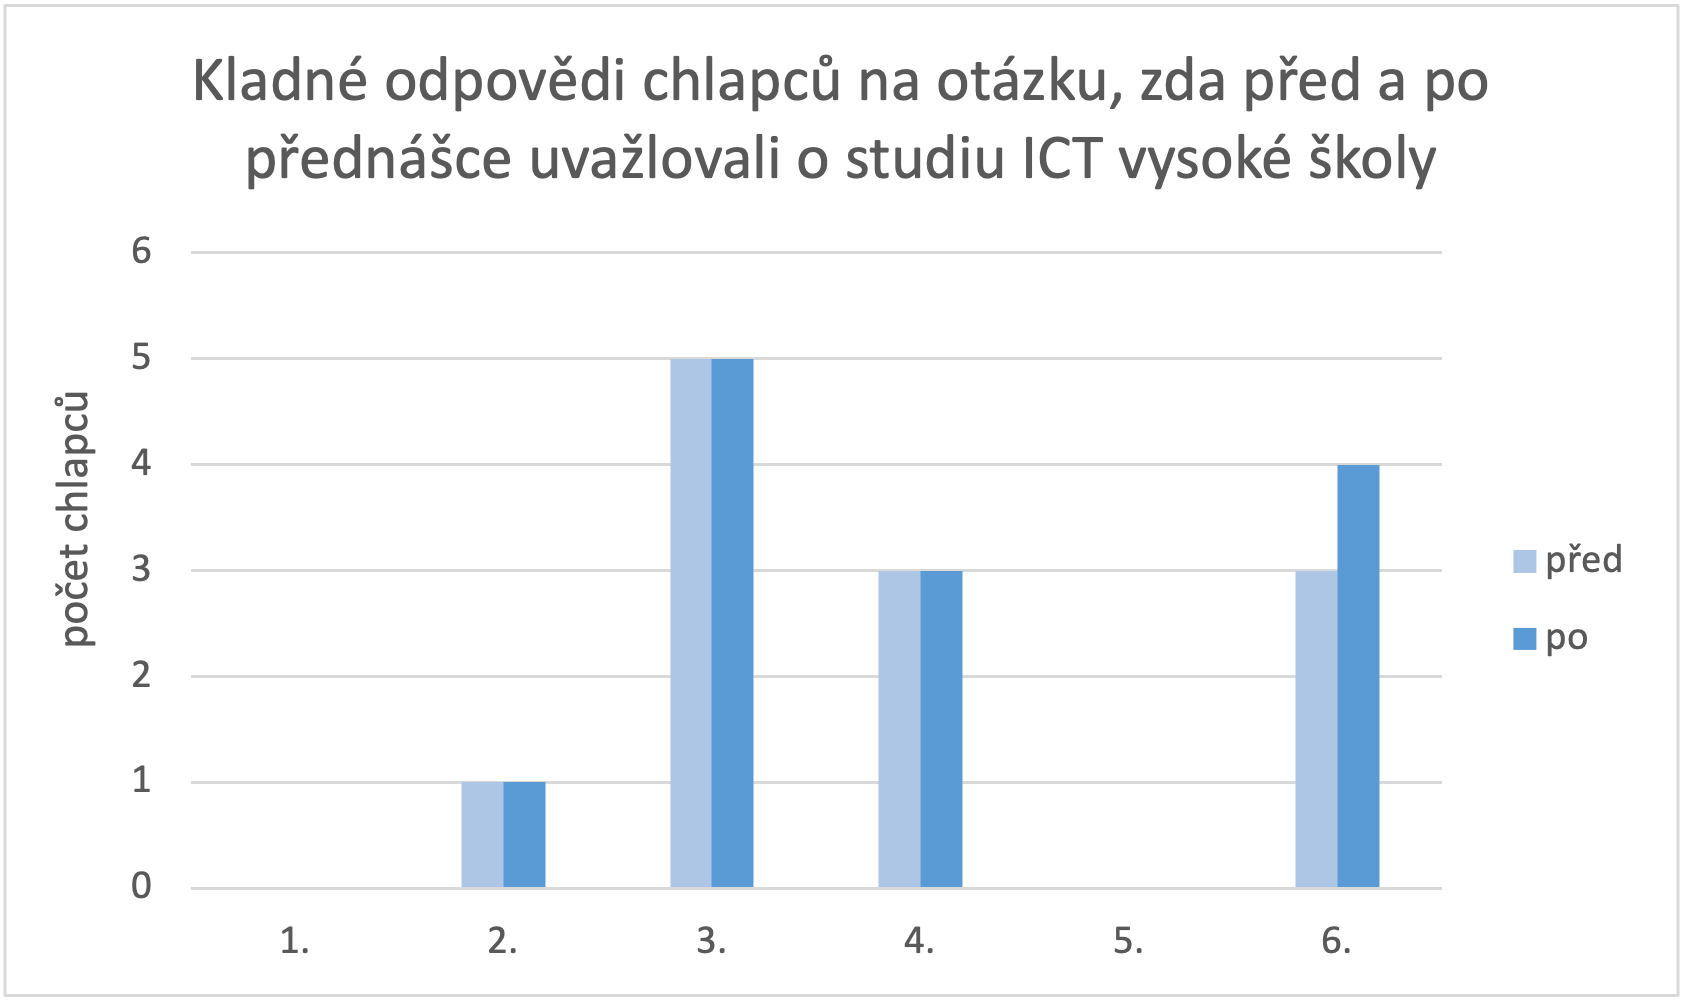
\includegraphics[width=16cm]{Maturitni Prace/images/chlapci_uvazovani.png} 
                    \caption{Počet kladných odpovědí od chlapců na otázku, zda před a po přednášce uvažovali o studiu na ICT VŠ}
                    \label{fig:chlapci_uvazovani}
                \end{figure}
                \begin{figure}
                    \centering
                    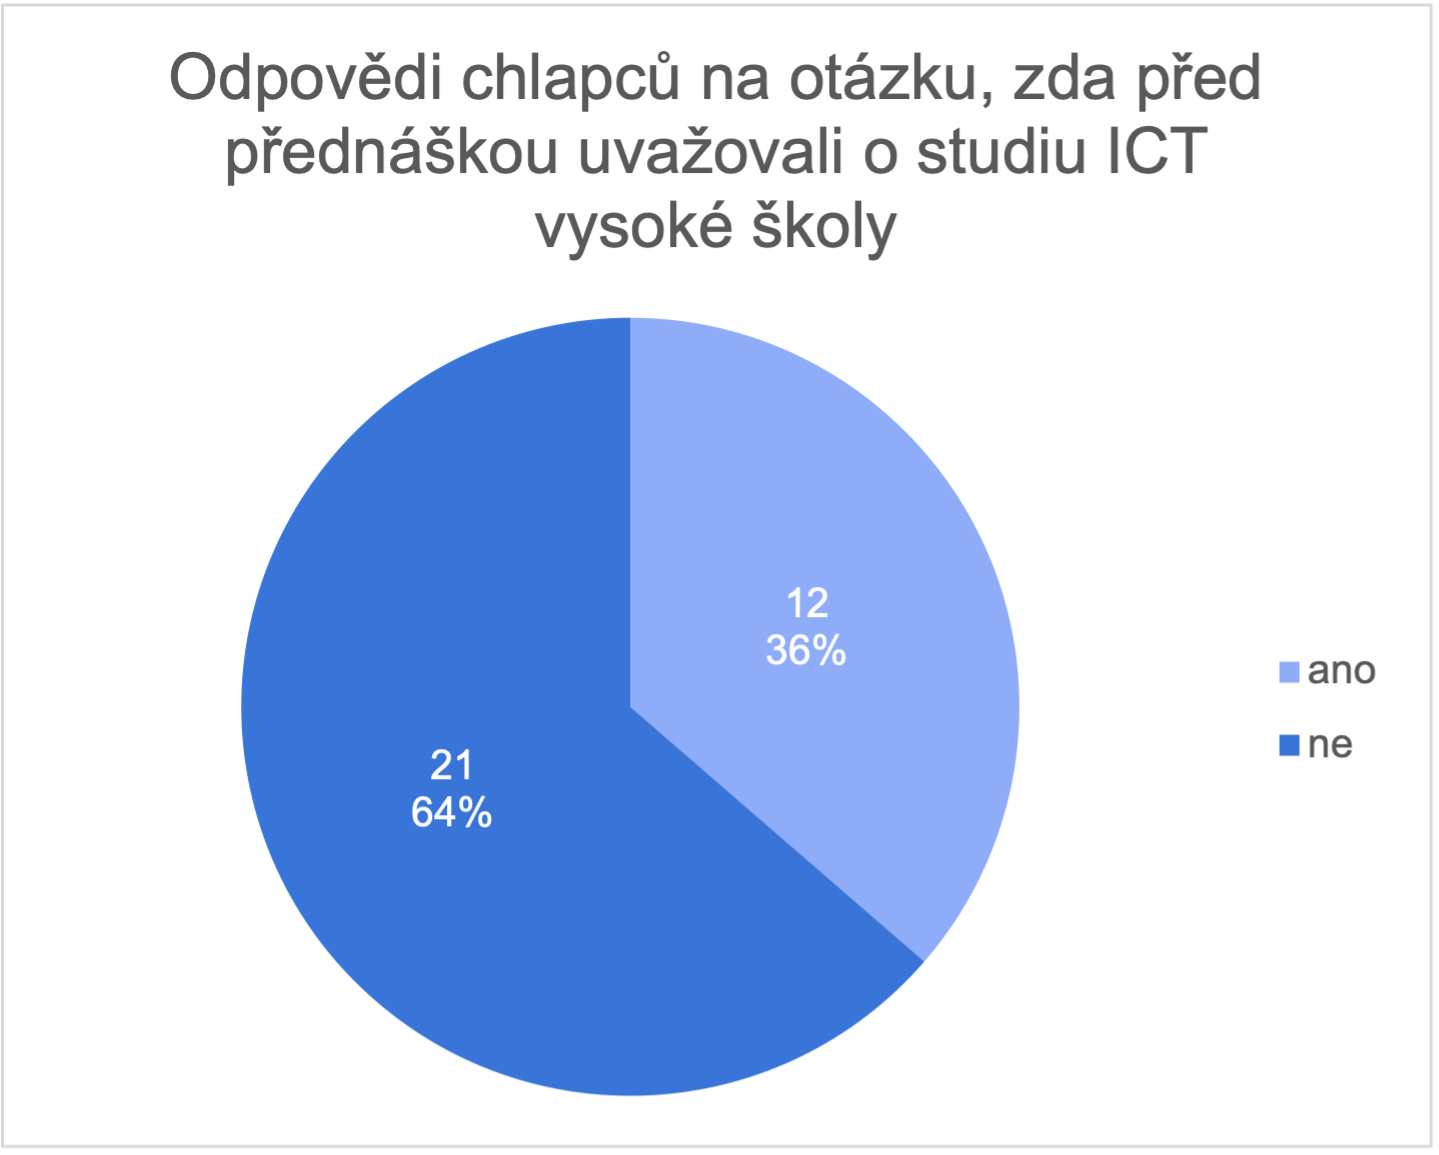
\includegraphics[width=8cm]{Maturitni Prace/images/chlapci_pred.png} 
                    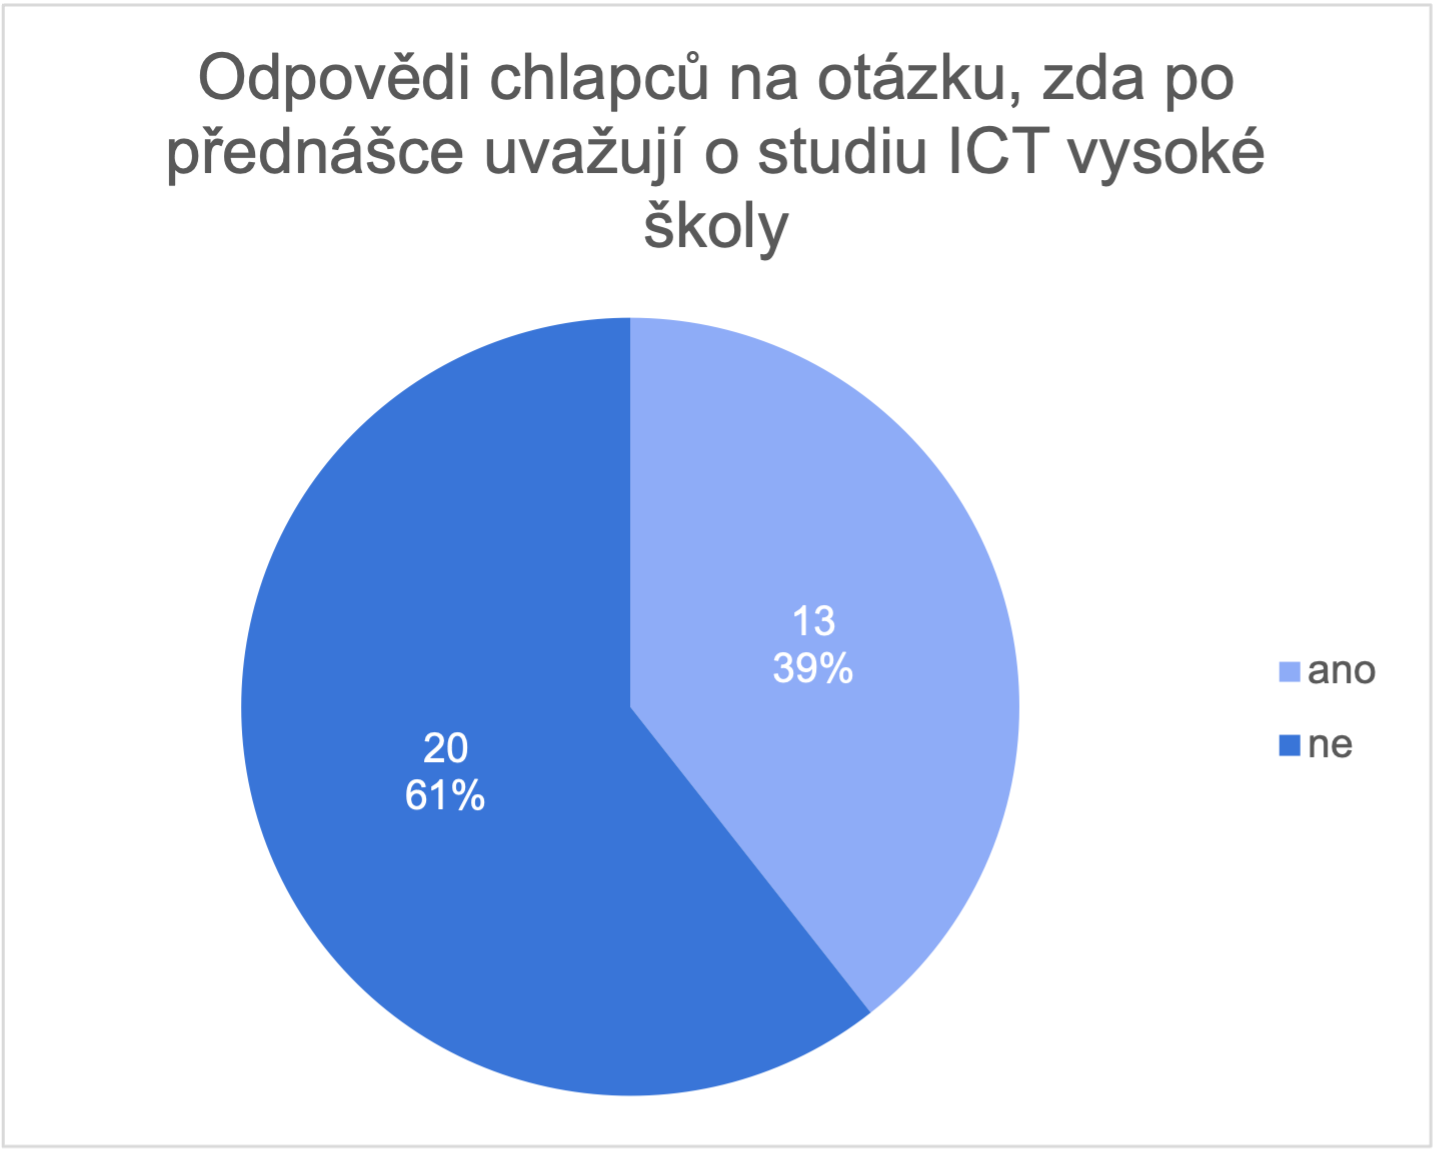
\includegraphics[width=8cm]{Maturitni Prace/images/chlapci_po.png} 
                    \caption{Odpovědi od dívek před a po provedených přednáškách na otázku zda uvažují o studiu na ICT VŠ}
                    \label{fig:chlapci}
                \end{figure}
                
                Pro porovnání jsem zpracovala i data co se týkají chlapců, která ale nejsou moc vypovídající, jelikož si z přednášky spíše než uvažování o studiu v tomto směru měli odnést, jak se v tomto ohledu chovat k dívkám, které o tomto směru uvažují. To v dotazníku nebylo a navíc tento způsob k tomu ani není vhodný. Graf (obr.: \ref{fig:chlapci_uvazovani}) nám tedy ukazuje, že přednáška ovlivnila pouze jednoho chlapce a to na poslední přednášce.  
                
                Pro porovnání opět situace před a po přednášce, jde hlavně o procentuální porovnání se situací u dívek, kdy můžeme vidět, že už před přednáškou o studiu informatiky na vysoké škole uvažovalo o 11\% více chlapců než dívek po přednášce (obr.: \ref{fig:chlapci}).
                

	\chapter*{Diskuze a závěr}
	    \section{Zhodnocení teoretické části}
	    
	        Práce se zaměřuje na téma diverzity. Jedna z hypotéz zněla \textit{\uv{Pandemie měla vliv na studenty a studentky ve výběru vysoké školy. O proti minulým letům se navýšil nejen počet studentů, kteří podali přihlášku na informatickou vysokou školu, ale i procento dívek, a to jak v počtu poslaných přihlášek, tak v počtu přijatých studentek}}. Díky datům poskytnutými přímo fakultou ČVUT byla možnost porovnat situaci právě na určitých fakultách namísto celonárodního průměru. I přesto, že počet studentů na všech vysokých školách v ČR klesal v období pandemie Covid-19 spíše stagnoval. ICT obor se dlouhodobě stává velmi oblíbeným. Zajímavostí je ale velký nárůst podaných přihlášek na akademický rok 2022/2023, podaných na začátku roku 2022. Navýšení se tedy nedá přímo spojit s pandemií Covid-19, jelikož je reakce studentů opožděná, ale i přesto takový nárůst všech přihlášek a dívek není náhodou. Bohužel zda zvýšený nárůst odeslaných přihlášek měl také vliv na počet přijatých studentů nebylo možné posoudit z důvodu nedostatku dat.
            
            Má druhá hypotéza se týkala pohlaví a jeho vliv na zaměstnání v ICT odvětví. \uv{Na získání práce v IT má větší vliv úroveň dosaženého vzdělání a pohlaví, než věk.}. Celá hypotéza je velmi rozsáhlá. Co se týká věku podle dostupných dat bych řekla, že věk je hodně ovlivněn tím, že je obor velmi mladý. Tedy nejvíce zastoupenou věkovou kategorií jsou lidé mezi 30 a 39 let věku, ale žádná z věkových kategorií, které je tento směr blízký (do 50 let) není diskriminována. Zatímco dosažené vzdělání má na zaměstnání vliv pokud se ucházíte od pozici ICT specialisty, zatímco u ICT techniků má více než polovina jako nejvyšší dosažené vzdělání střední školu s maturitou u ICT specialistů je situace opačná a více než 80\% zaměstnanců má jako nejvyšší dosažené alespoň bakalářské či vyšší odborné vzdělání. Co se týká pohlaví, má na získání práce v tomto odvětví největší vliv, jelikož je společností vnímáno jako \uv{pro muže}. Zároveň ale z historie víme, že ženy do ICT patřily. Celou hypotézu bych potvrdila, jelikož věk má opravdu na zaměstnání v tomto oboru nejmenší vliv.
	    
	    \section{Zhodnocení přednášek}
            
            U přednášek nám šlo hlavně o oslovení co nejvíce studentů a ovlivnit co nevíce dívek alespoň k uvažování o studiu informatiky na vysoké škole. \textit{\uv{ Přednášky ovlivní alespoň jednu dívku, která před přednáškou neuvažovala o studiu
            informatiky.}} Celkem se nám tedy dohromady ve 4 podařilo oslovit přibližně 950 žáků. Já sama jsem oslovila přibližně 450 žáků. Zpětnou vazbu po přednášce jsem obdržela od 128 z nich. Kde 89 bylo dívek z nichž celkem 10 dívek (12\%) začalo po přednášce uvažovat o studiu ICT VŠ. Pokud bychom tuto statistiku aplikovali na všechny žáky pro které jsem přednášela. Procentuálně pokud by bylo 69\% z žáků dívek, je zde pravděpodobnost, že jsem celkem ovlivnila něco okolo 37 dívek a 4 chlapce. 
            
            Není to ale jediná informace, kterou jsem z přednášek získali. Dalo se očekávat, že zájem chlapců o tento směr bude vyšší než u dívek. Podle dat získaných z přednášek tomu tak opravdu bylo, ale ten rozdíl mezi zájmem chlapců o následné studium v tomto oboru je už před samotnou přednáškou o 11\% vyšší než po přednášce u dívek. Po přednášce je rozdíl ještě markantnější. 
            
            Já osobně jsem si z celé praktické části odnesla hodně, jelikož jsem měla možnost pracovat na projektu od začátku  až po samotné přednášky. Velmi mě bavil proces tzv. brainstormingu, kde bylo pozitivně nahlíženo na jakýkoliv nápad. A také pro mě byla velká zkušenost přednášet až pro 120 studentů středních škol, ze které budu hodně čerpat do budoucích prezentací.
            )   
        \section{Závěr}
         Cílem práce bylo zhodnocení diverzity na vysokých školách a v zaměstnání. Celkově si myslím, že zpracování je dostatečně komplexní pro pochopení celé problematiky i pro neznalého člověka. Co se týká hypotéz, podařilo se mi dvě z nich přímo prokázat, pro třetí nebylo dostatek dat. I přesto beru celou práci za velmi užitečnou.
	

	\nocite{*}
    \printbibliography					% Vytvoří seznam literatury
	\addcontentsline{toc}{chapter}{Bibliografie}
    \listoffigures						% Vytvoří seznam obrázků
    \begin{appendices}
	\chapter{Prezentace}
	    
	    \begin{figure}[h]
            \centering
            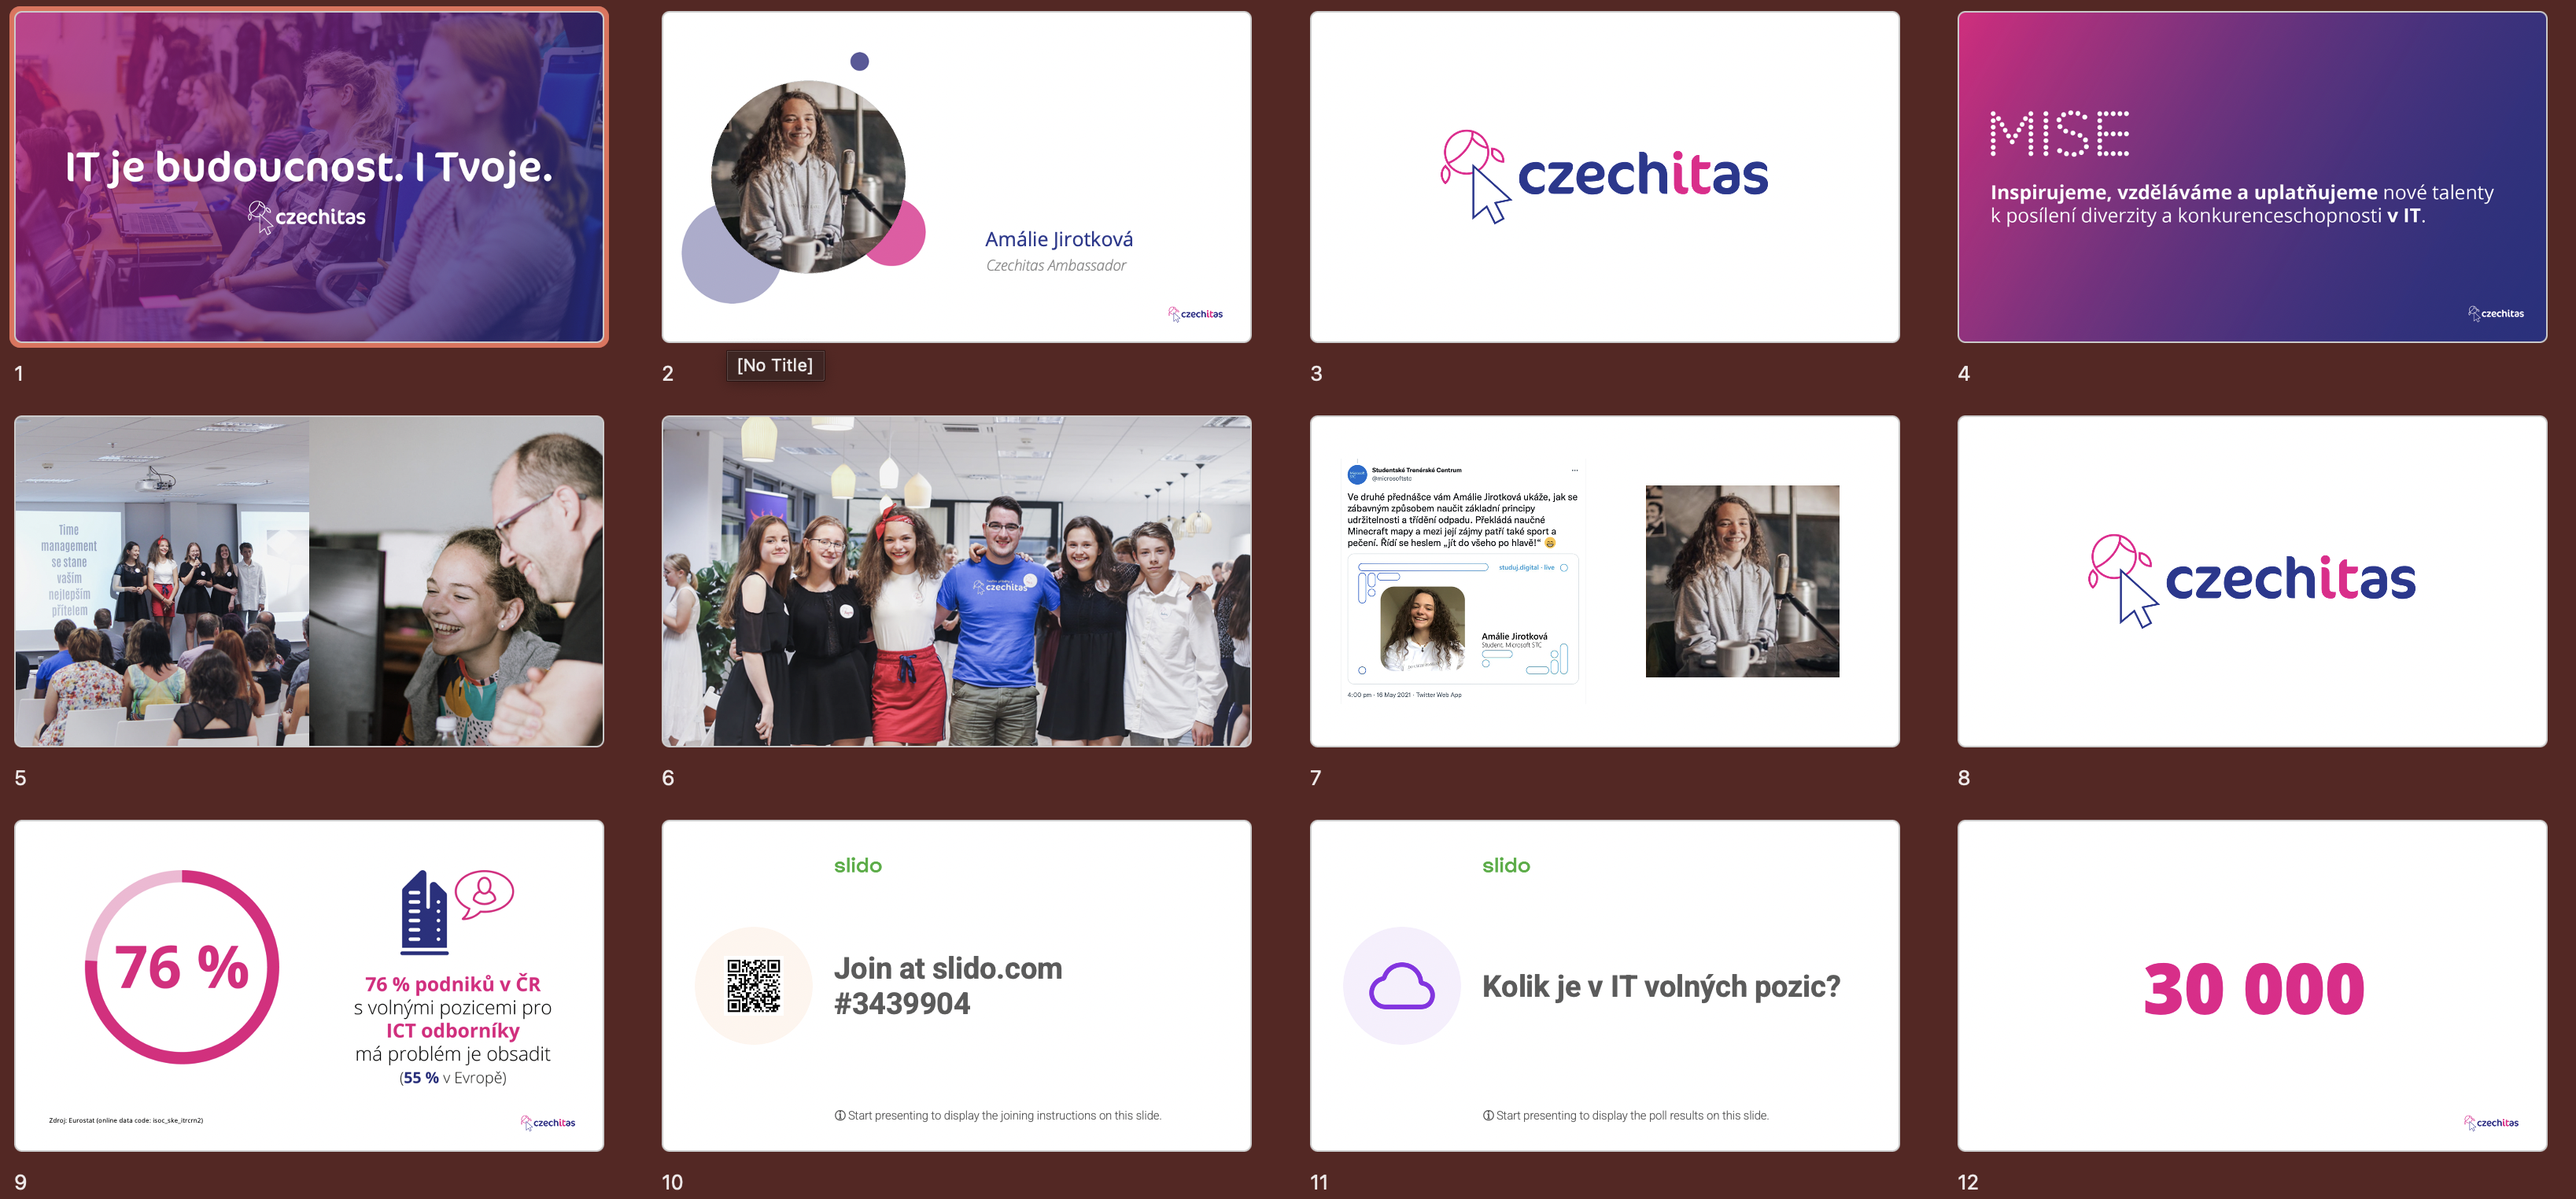
\includegraphics[width=16cm]{Maturitni Prace/images/Screenshot 2023-01-29 at 19.09.06.png} 
            \caption{Prezentace přednášená pro studenty; Zdroj: Czechitas}
            \label{fig:prezentace_1}
        \end{figure} 
        
        \begin{figure}[h]
            \centering
            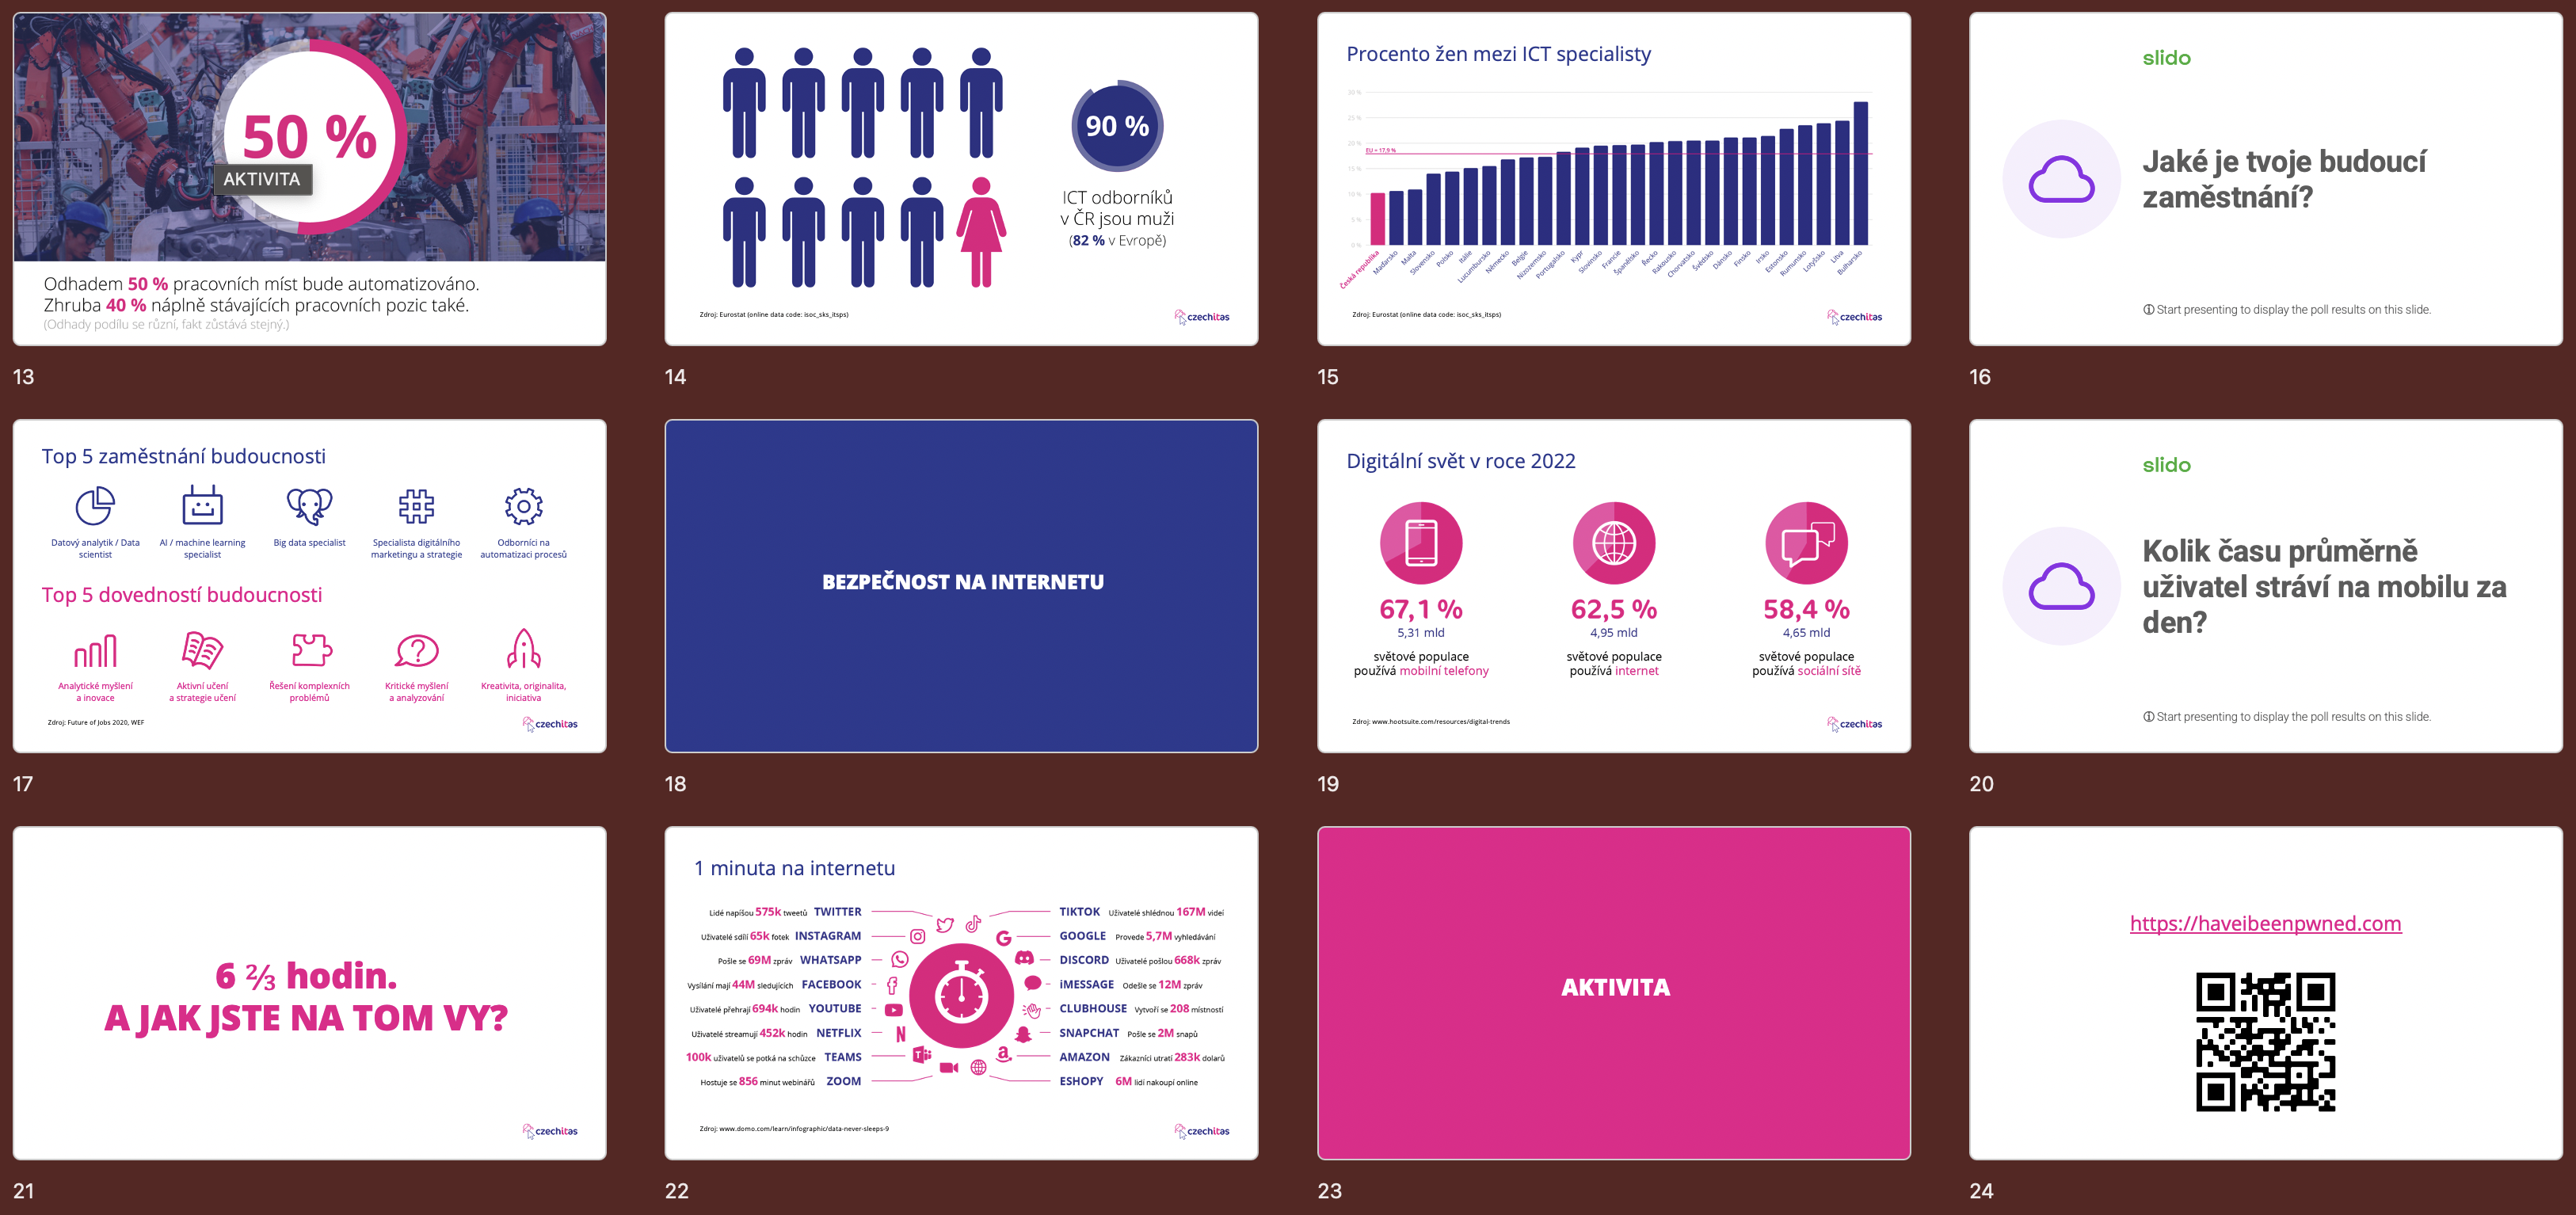
\includegraphics[width=16cm]{Maturitni Prace/images/Screenshot 2023-01-29 at 19.09.25.png} 
            \caption{Prezentace přednášená pro studenty; Zdroj: Czechitas}
            \label{fig:prezentace_2}
        \end{figure} 
        
        \begin{figure}[h]
            \centering
            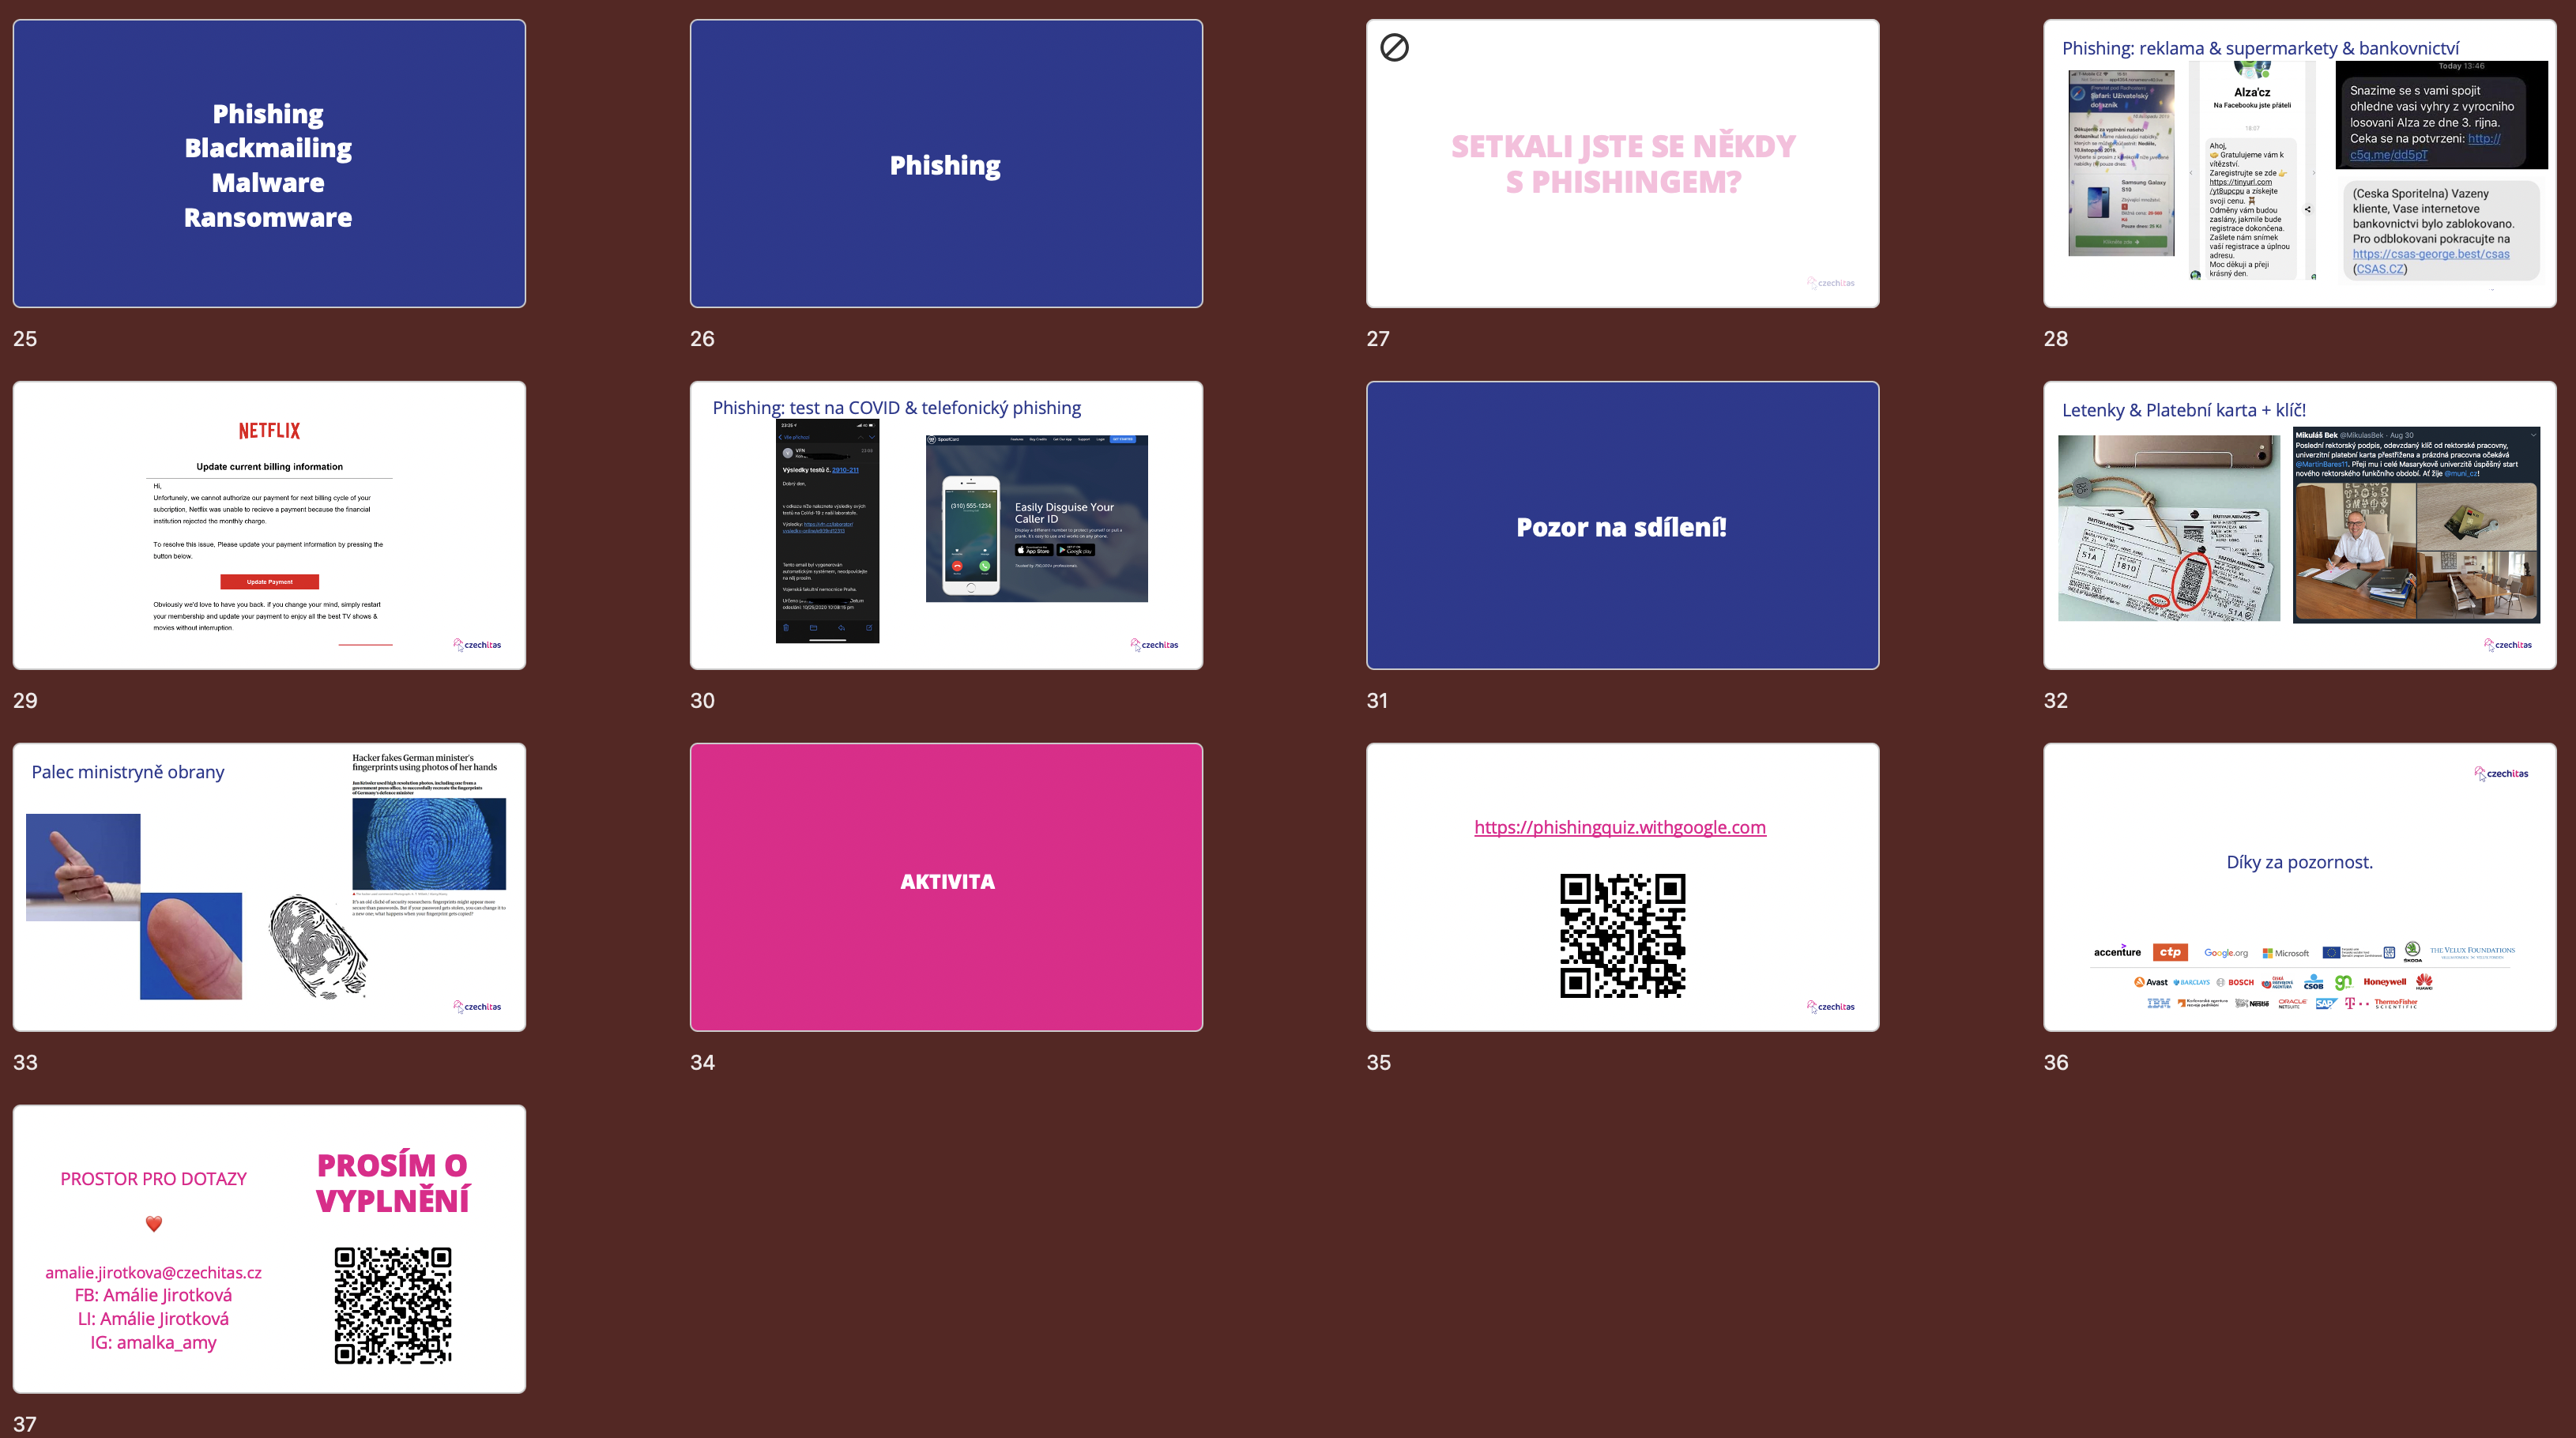
\includegraphics[width=16cm]{Maturitni Prace/images/Screenshot 2023-01-29 at 19.09.57.png} 
            \caption{Prezentace přednášená pro studenty; Zdroj: Czechitas}
            \label{fig:prezentace_3}
        \end{figure} 
        
        %@online{Forbes,
        %    	title     = "Dita Přikrylová je v 30 pod 30!",
        %    	journal   = "Forbes CZ",
        %        url       = "http://www.forbes.cz/30pod30-2016/23-prikrylova"
        %    }
        
	\end{appendices}
\end{document}

